\chapter{Analysis}
\label{ch:analysis}
\graphicspath{{Chapter-Analysis/figures/}}

\section{Data set}

The analyses presented in this thesis use the data from the 2013 \pPb run at the \ac{LHC} with a center-of-mass energy of \pPbenergy for a total integrated luminosity of \pPblumi.
The Pb ions had an energy per nucleon of $1.57 \TeV$ and collided with the $4 \TeV$ proton beam resulting in a net longitudinal boost of the center-of-mass system of $\ycm = 0.465$ in the proton direction relative to the ATLAS laboratory frame.
The \pPb\ run was divided into two periods between which the directions of the proton and lead beams were
reversed. 
The data are presented using the convention that the proton beam travels in the forward ($+z$) direction and the lead beam travels in the backward ($-z$) direction.
When the data from these two periods are combined, the \minbias triggers sampled a total luminosity, after prescale, of $24.5~\mu\textrm{b}^{-1}$ and yielded a total of 44 million events over the full centrality.

For results reported as a function of centrality, an additional \ac{HighET} trigger selection is included in the most central bin that requires the total transverse energy in both sides of the \ac{FCal} to be at least 65 \GeV.
The \ac{HighET} trigger sampled a total luminosity of $41.4~\mu\textrm{b}^{-1}$ after prescale and yielded 700 thousand events to the sample.
Events from this trigger are only included in the 0--1\% centrality interval, where the \ac{HighET} trigger is fully efficient.

Several \acp{HMT} are included to boost the sample used in the azimuthal analysis, with offline \Nch cutoffs at 100, 130, 150, 180, 200, and 225 tracks.
These \acp{HMT} provide a crucial 6.7 million events, as the \minbias triggers provide only 200 000 events at $\Nch \geq 150$.

All events are required to pass a set of \minbias selection criteria.
Events are required to be included in the latest Good Runs List from ATLAS, which rejects events recorded in conjunction with a technical difficulty in the detector.
The \minbias trigger requires either one hit in both sides of the \ac{MBTS} or two hits in one side.
Additional \ac{HighET} and high multiplicity triggers are included in some analysis bins as discussed above.
%% Events with an offline multiplicity lower than the nominal trigger threshold are excluded, as each of these HMTs reaches an efficiency near 1 near their nominal turn-on. This rejects events that fire a trigger in its turn-on region, as these samples can in principle be biased.
%% In practice no significant difference in the results is observed whether or not events in the HMT triggers' turn-ons are included, so using the nominal turn-on multiplicity is sufficient.
A timing cut is placed on the \ac{MBTS} hits in each side such that $|\Delta t_{AC}| < 10~\textrm{ns}$.
No more than one reconstructed \ac{PV} or strong vertex (where a strong vertex has more than 10 tracks or a total \pt of tracks greater than $6~\GeV$) is permitted in each event.
Diffractive events are identified for rejection by a gap of two units of pseudorapidity in event activity on the Pb-going side of the calorimeters \cite{HION-2012-15}.
Pileup events are also discarded using a run-dependent upper limit on the Pb-going \ac{ZDC}.
In addition, events are discarded if an error flag is recorded in the \ac{LAr} or tile calorimeter systems, or if there is an indication that the event was not completely recorded.

\subsection{Centrality determination}

\begin{figure}[t]
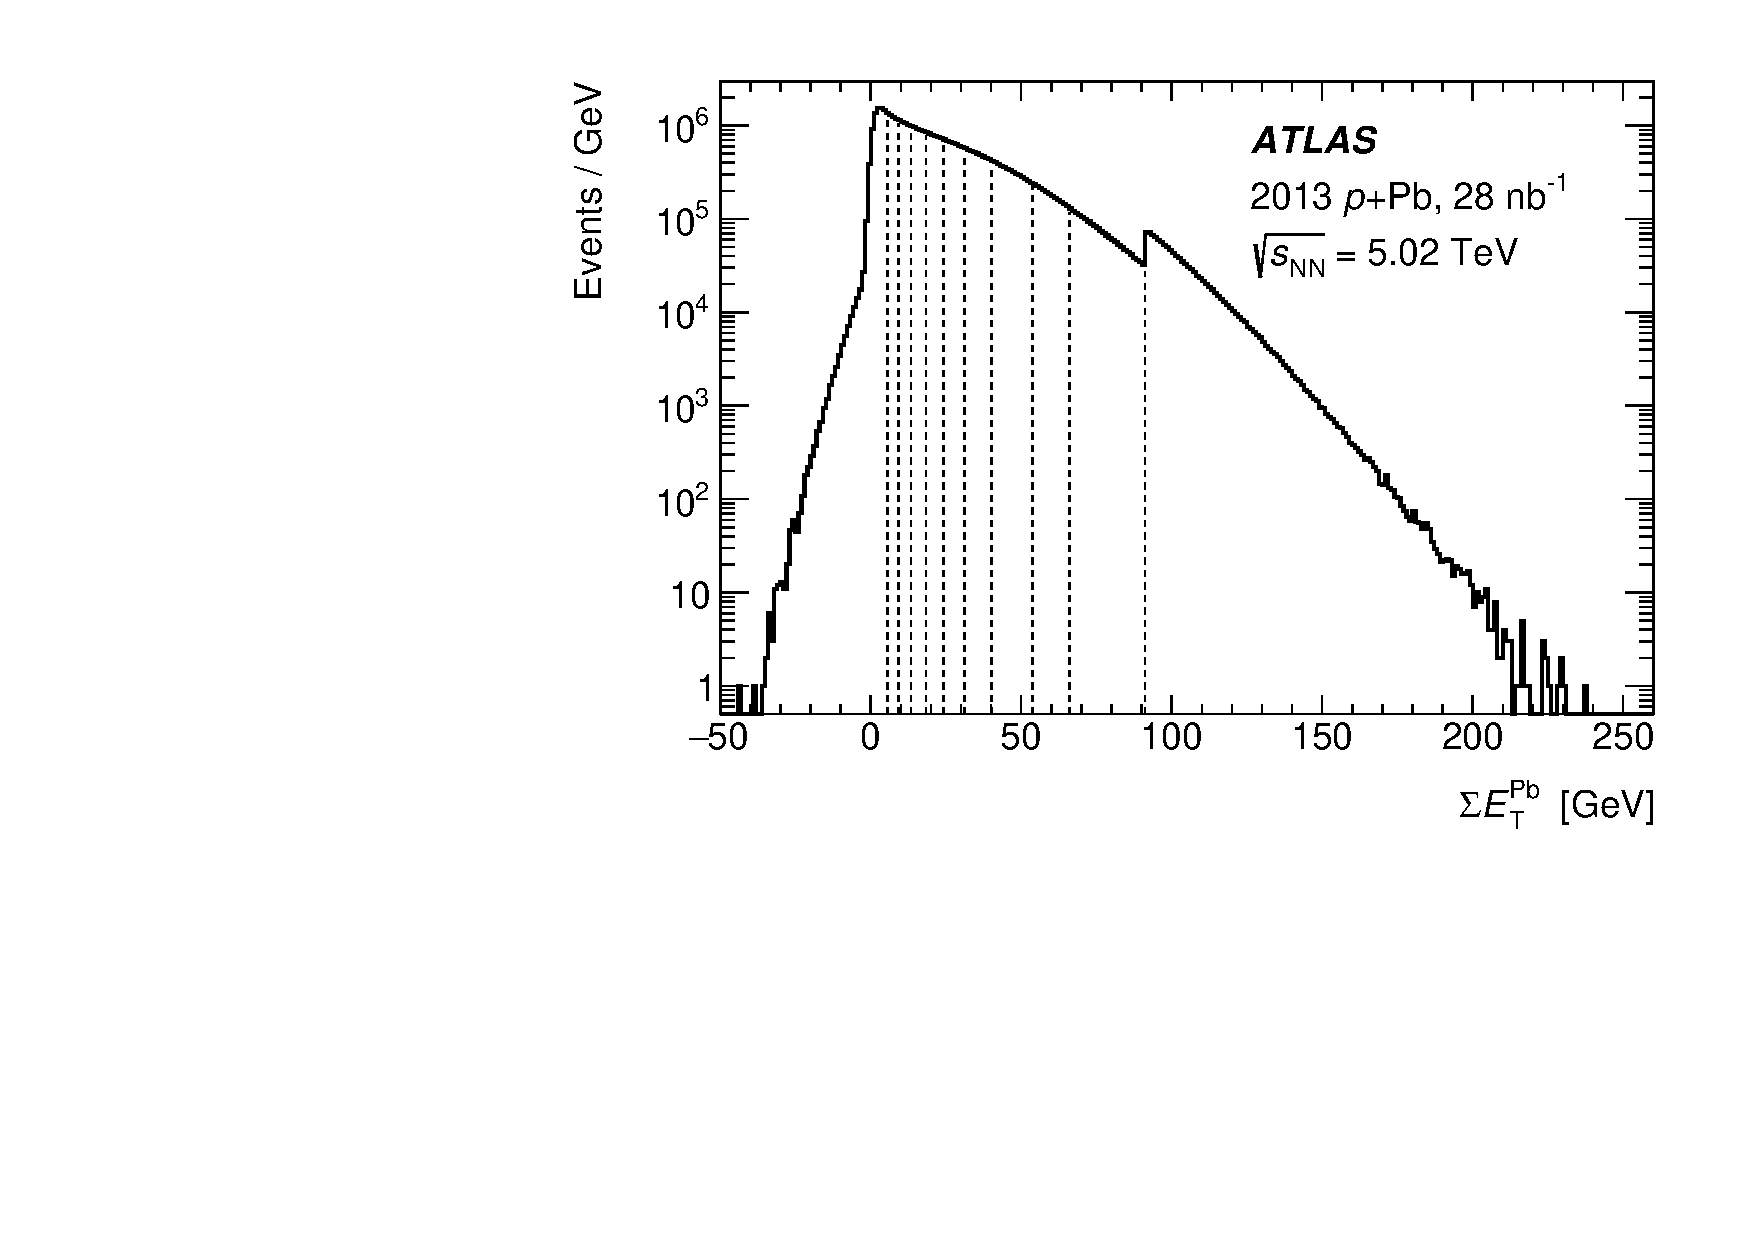
\includegraphics{fcal_et_total.pdf}
\caption{The distribution of the total transverse energy in the \ac{FCal} in the Pb-going direction (\sumETPb) for the events used in the centrality-dependent analysis. Dashed lines are shown at the boundaries of the centrality intervals, and the discontinuity at $\sumETPb = 91.08~\GeV$ corresponds to the lower \sumETPb boundary of the 0--1\% centrality interval. Negative values can occur because the mean noise is subtracted from each calorimeter cell.}
\label{fig:fcal_et}
\end{figure}

The centralities of the \pPb\ events are characterized following the procedures described in \Ref{\cite{HION-2012-15}}, using the total transverse energy in the Pb-going side of the \ac{FCal}, \sumETPb.
The use of the \ac{FCal} for measuring centrality has the advantage that it is not sensitive to multiplicity fluctuations in the kinematic region covered by the inner detector, where the measurements are performed.
Measurements are presented in this paper for the centrality intervals listed in \cref{table:npart}.
The events selected using the \ac{HighET} trigger are used only in the 0--1\% centrality interval.
\cref{fig:fcal_et} shows the distribution of \sumETPb\ values obtained from events included in this
measurement.
The discontinuity in the spectrum occurs at the low edge of the 0--1\% centrality interval, above which the \ac{HighET} events are included.

For each centrality interval, the average multiplicity of charged particles with $\pt > 100~\MeV$ and $|\eta| < 1.5$, \avgdNdeta and the corresponding average number of participating nucleons, \avgNpart, are obtained from a previous publication \cite{HION-2012-15}.
Since this analysis uses finer centrality intervals (no wider than 10\% of the total centrality range) than
those used in \Ref{\cite{HION-2012-15}}, a linear interpolation over the Glauber \avgNpart is used to construct additional values for \avgdNdeta based on the published results.
This interpolation is justified by the result in \Ref{\cite{HION-2012-15}} that charged-particle multiplicity is proportional to \avgNpart in the peripheral region.
The values and uncertainties from this procedure are listed in \cref{table:npart}.


\renewcommand{\arraystretch}{1.1}
\begin{table}
\begin{center}
\begin{tabular}{r || c | c | c || c}
\hline
 & \multicolumn{3}{c||}{\avgNpart} & \\ \cline{2-4}
Centrality & Glauber & GGCF $\omega_{\sigma} = 0.11$ & GGCF $\omega_{\sigma} = 0.2$ & $\avgdNdeta$\\
\hline \hline
0--1\% & $ 18.2^{+2.6}_{-1.0} $ & $ 24.2^{+1.5}_{-2.1} $ & $ 27.4^{+1.6}_{-4.5} $ & $58.1\ \pm 0.1\ \ \pm 1.9\ $ \\[2pt]
\hline
1--5\% & $ 16.10^{+1.66}_{-0.91} $ & $ 19.5^{+1.2}_{-1.3} $ & $ 21.4^{+1.5}_{-2.0} $ & $45.8\ \pm 0.1\ \ \pm 1.3\ $ \\[2pt]
\hline
5--10\% & $ 14.61^{+1.21}_{-0.82} $ & $ 16.5^{+1.0}_{-1.0} $ & $ 17.5^{+1.1}_{-1.1} $ & $38.5\ \pm 0.1\ \ \pm 1.1\ $ \\[2pt]
\hline
10--20\% & $ 13.05^{+0.82}_{-0.73} $ & $ 13.77^{+0.79}_{-0.81} $ & $ 14.11^{+0.86}_{-0.79} $ & $32.34 \pm 0.05 \pm 0.97$ \\[2pt]
\hline
20--30\% & $ 11.37^{+0.65}_{-0.63} $ & $ 11.23^{+0.62}_{-0.67} $ & $ 11.17^{+0.68}_{-0.62} $ & $26.74 \pm 0.04 \pm 0.80$ \\[2pt]
\hline
30--40\% & $ 9.81^{+0.56}_{-0.57} $ & $ 9.22^{+0.50}_{-0.54} $ & $ 8.97^{+0.60}_{-0.49} $ & $22.48 \pm 0.03 \pm 0.75$ \\[2pt]
\hline
40--50\% & $ 8.23^{+0.48}_{-0.55} $ & $ 7.46^{+0.41}_{-0.43} $ & $ 7.15^{+0.54}_{-0.39} $ & $18.79 \pm 0.02 \pm 0.69$ \\[2pt]
\hline
50--60\% & $ 6.64^{+0.41}_{-0.52} $ & $ 5.90^{+0.36}_{-0.34} $ & $ 5.60^{+0.47}_{-0.30} $ & $15.02 \pm 0.02 \pm 0.62$ \\[2pt]
\hline
60--70\% & $ 5.14^{+0.35}_{-0.43} $ & $ 4.56^{+0.32}_{-0.26} $ & $ 4.32^{+0.41}_{-0.23} $ & $11.45 \pm 0.01 \pm 0.56$ \\[2pt]
\hline
70--80\% & $ 3.90^{+0.24}_{-0.30} $ & $ 3.50^{+0.22}_{-0.18} $ & $ 3.34^{+0.29}_{-0.16} $ & $ \ \  8.49 \pm 0.02 \pm 0.51$ \\[2pt]
\hline
\end{tabular}
\caption{The average number of nucleon participants \avgNpart \cite{HION-2012-15} for each centrality interval in the Glauber model as well as the two choices for the Glauber-Gribov model with color fluctuations (GGCF) \cite{Alvioli:2013vk} (and references therein), along with the average multiplicity with $\pt > 100~\MeV$ and $|\eta| < 1.5$ also obtained from Ref.~\cite{HION-2012-15}. The parameter $\omega_{\sigma}$ represents the size of fluctuations in the nucleon-nucleon cross section. Asymmetric systematic uncertainties are shown for \avgNpart. The uncertainties in \avgdNdeta are given in the order of statistical followed by systematic.}
\label{table:npart}
\end{center}
\end{table}

 

\subsection{Multiplicity selection}

\begin{figure}[t]
\centering
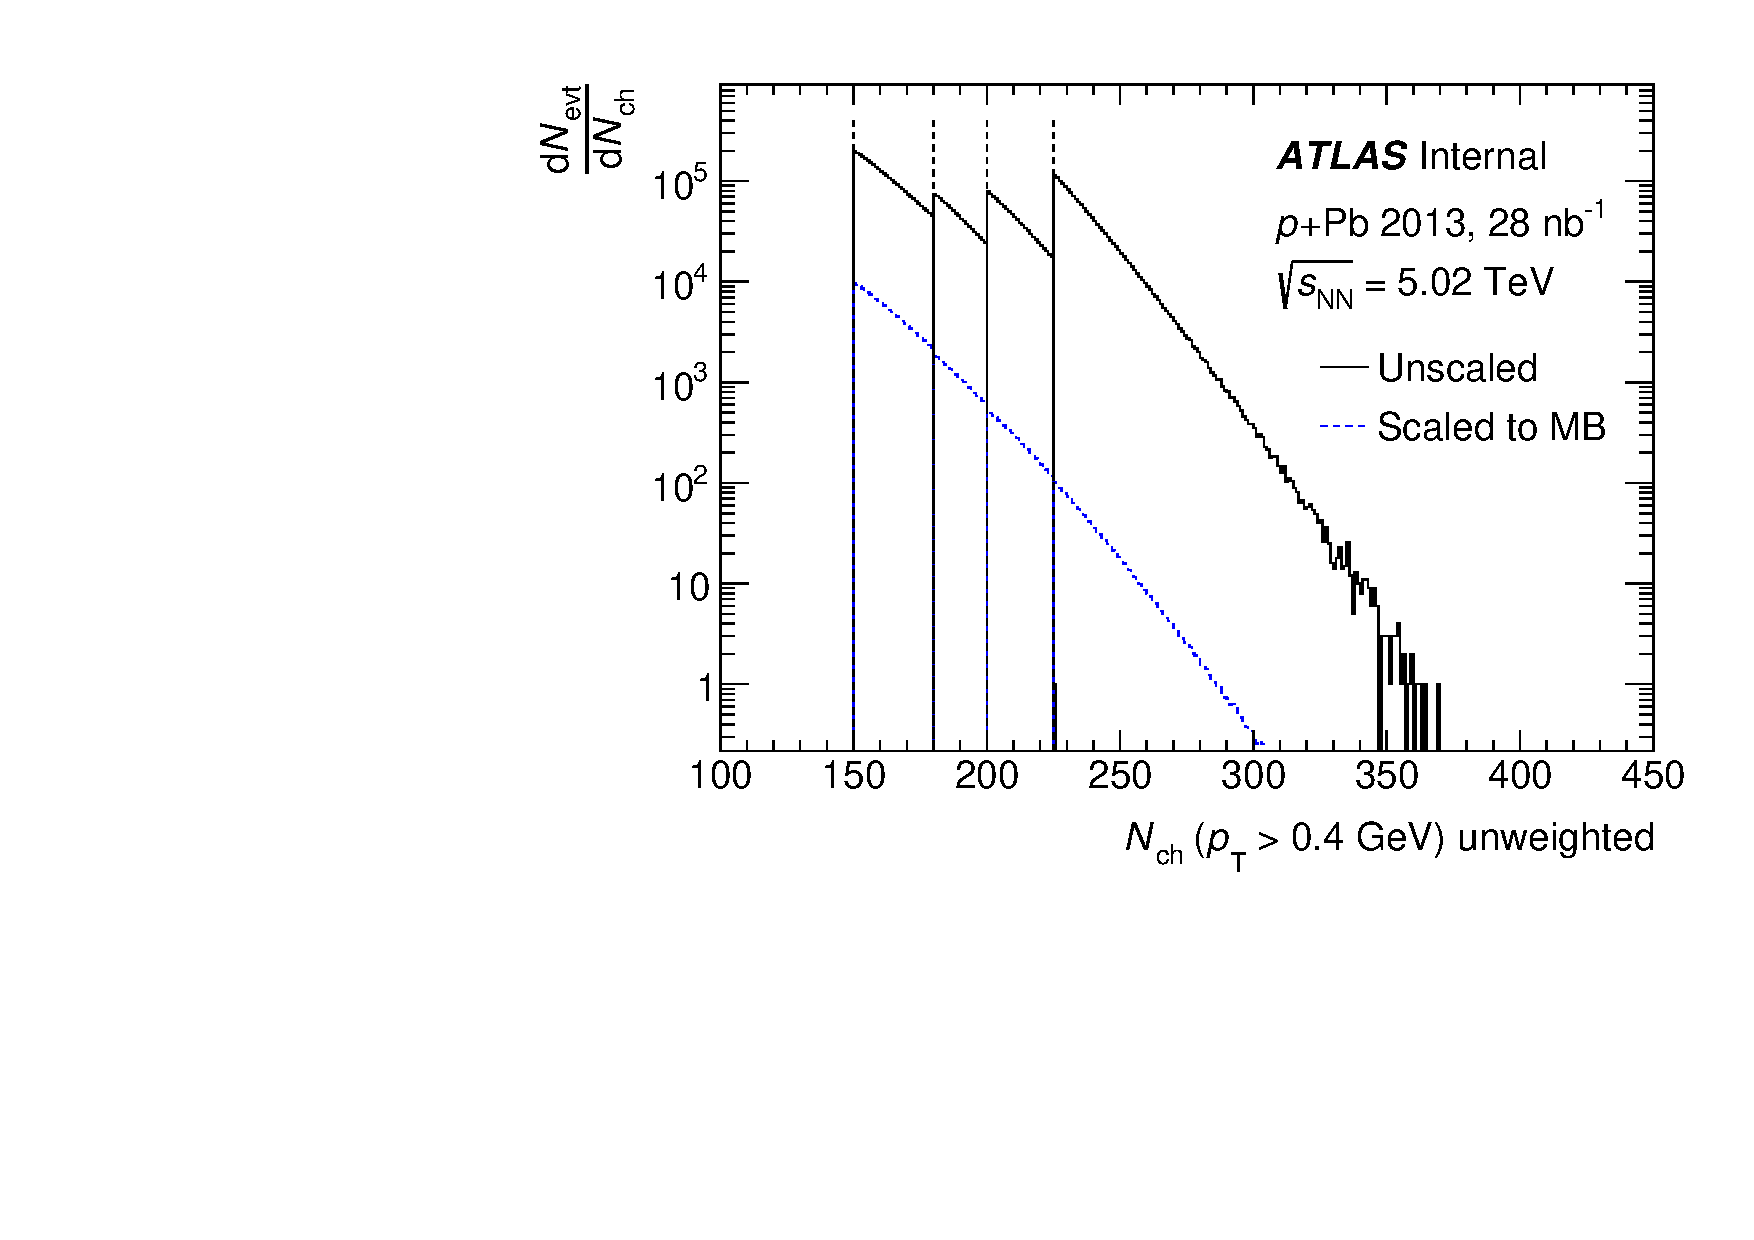
\includegraphics{can_nch.pdf}
\caption{The charged-particle multiplicity \Nch of tracks with $\pt > 0.4$ GeV. Each of the four cutoffs corresponds to additional triggers used in the analysis. The distribution scaled down to match the scale of the events from the MinBias trigger is also shown by the dashed blue line.}
\label{fig:nch}
\end{figure}

For the azimuthally-dependent results, events are selected by their reconstructed charged-particle multiplicity \Nch, with a minimum value of 150.
Tracks are only counted towards \Nch if they have $\pt > 400 \MeV$, where the reconstruction efficiency is relatively constant.
This choice permits the straightforward inclusion of several \acp{HMT} into the sample, which is particularly useful because only central events allow a sufficiently high event plane resolution.
The multiplicity distribution is shown in \cref{fig:nch} along with a scaled version to match the \minbias distribution.

%% ---------------------------------
%% event plane determination
%% ---------------------------------
\section{Flow vector determination}

The 2nd-order azimuthal Fourier components $Q_2$ of the energy flow are defined by
\begin{equation}
  Q_2 = \sum_{i}  \et{}_i \begin{pmatrix} \cos 2\phi_i \\ \sin 2\phi_i \end{pmatrix} \; ,\\
\end{equation}
where the sum is taken over calorimeter cells and $\phi_i$ is the ATLAS detector coordinate $\phi$ of the $i$th calorimeter cell.
The two-component elliptic flow vector \qt is defined in terms of $Q_2$, normalized by the 0th-order Fourier component
\begin{equation}
  \qt = \frac{Q_2}{\sum_i \et{}_i } \; .\\
\end{equation}
The elliptic flow used in this analysis is taken from calorimeter cells on the Pb-going side of the detector with $\eta < -2.5$ for period B or $\eta > 2.5$ for period A, which has the beam orientation reversed.
This forward cut is made so as to not overlap with the inner detector.

The second-order event plane angle \psit is defined as
\begin{equation}
2\psit = \mathrm{atan2}(\qt{}_{,y},\qt{}_{,x})
\end{equation}
and is degenerate under $\psit \rightarrow \psit + \pi$.
The magnitude of the flow vector is $|\qt| = \sqrt{\qtx^2 + \qty^2}$; this is essentially a proxy for the total event flow $v_2$ but computed only in the forward region to remove auto-correlations with the inner detector.
An equivalent expression of these equations is
\begin{equation}
\qt = |\qt| e^{i2\psit} = \frac{\sum_i \et{}_i e^{i2\phi_i}}{\sum_i \et{}_i} \; .
\end{equation}
A sketch of the relationship of event plane angle to transverse momentum is shown in \cref{fig:ep_cartoon}.

\begin{figure}[t]
  \centering
  \includegraphics[width=\linewidth]{event_plane_cartoon.png}
  \caption{The event plane angle $\psit$ in relation to the elliptic moment of transverse energy. An exaggerated example of the transverse profile in a hydrodynamic system is shown in blue. The pressure gradients are larger along the axis of narrower extent, leading to greater final momentum in that direction.}
\label{fig:ep_cartoon}
\end{figure}

\subsection{First-order correction}
Due to non-uniformities in the calorimeter response the measurement of the \qt vector can be biased.
This leads to a non-uniform distribution of event plane angle \psit with an additive term proportional to $\cos [2(\psit - \phi_0)]$ which is obviously not physical.
This bias is corrected by subtracting off the mean \qt on a run-by-run basis.
The mean components of the \qt vector are shown in \cref{fig:mean_q2}.
The correction factors are statistically consistent in different multiplicity intervals, so all multiplicities are combined to increase their statistical significance.

\begin{figure}[t]
\centering
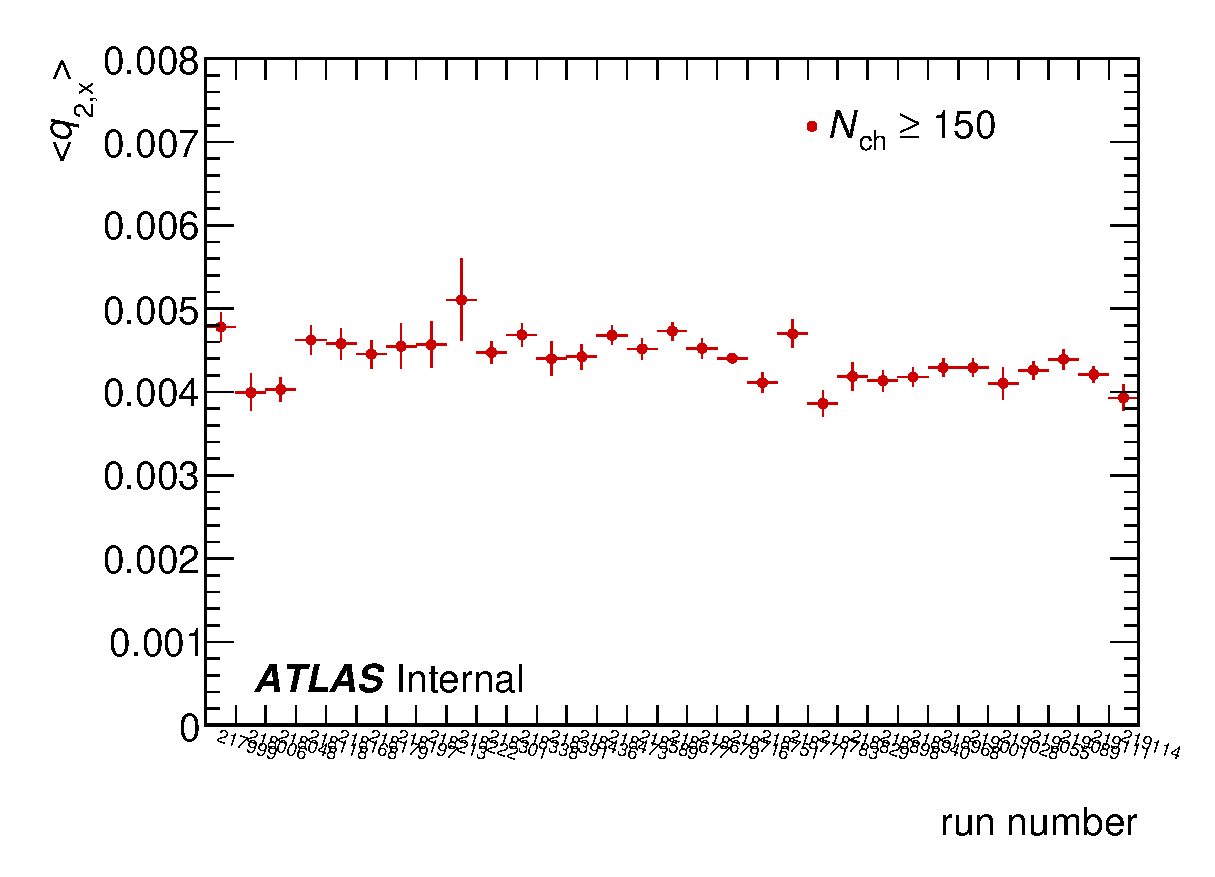
\includegraphics[width=.49\linewidth]{can_qx.eps}
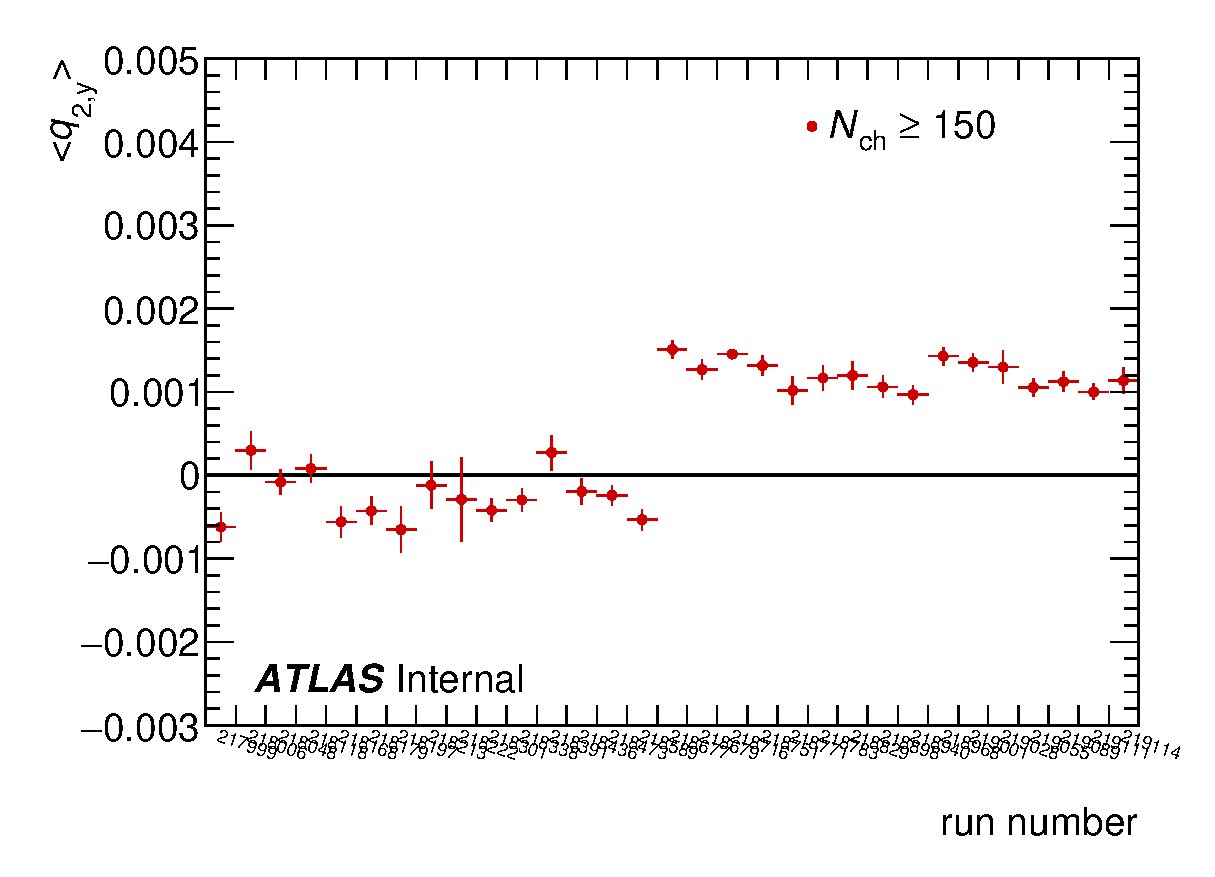
\includegraphics[width=.49\linewidth]{can_qy.eps}
\caption{The average components of the \qt vector $\langle\qtx\rangle$ (left) and $\langle\qty\rangle$ (right) for each run. Runs up to 218589 are from period A, and use $\eta > 2.5$, while runs after this are from period B and use $\eta < -2.5$.}
\label{fig:mean_q2}
\end{figure}

\subsection{Second-order correction}

Some additional non-uniformities persist in the \psit distribution even after correcting for the nonvanishing $\langle\qt\rangle$.
These contribute to higher-order Fourier terms like $\cos (4\psit)$ and $\sin(4\psit)$ in the distribution of the event plane angle \psit.
They arise because detector irregularities can lead to higher-order distortions in the distribution of the matrix of products $\qt{}_i \qt{}_j$.
In order to correct for these and make $\langle \qt{}_i \qt{}_j \rangle$ proportional to the identity matrix the mean-corrected \qt vector is multiplied by the normalized inverse square root of the covariance matrix
\begin{equation}
\frac{1}{\sqrt{N}} \left( \begin{array}{ccc}
  \langle \qty^2 \rangle + D & -\langle\qtx\qty\rangle \\
  -\langle\qtx\qty\rangle & \langle \qtx^2 \rangle + D
  \end{array} \right) \; ,
\end{equation}
where $D = \sqrt{\langle \qtx^2 \rangle \langle \qty^2 \rangle - \langle \qtx \qty \rangle ^2}$ and $N = D\left(\langle \qtx^2 \rangle + \langle\qty^2\rangle + 2D\right)$.
The components of the covariance matrix are shown in \cref{fig:mean_q2_cov}.
This multiplication removes the skew from the \qt distribution and causes it to have the same width in the \qtx and \qty axes.

\begin{figure}[t]
\centering
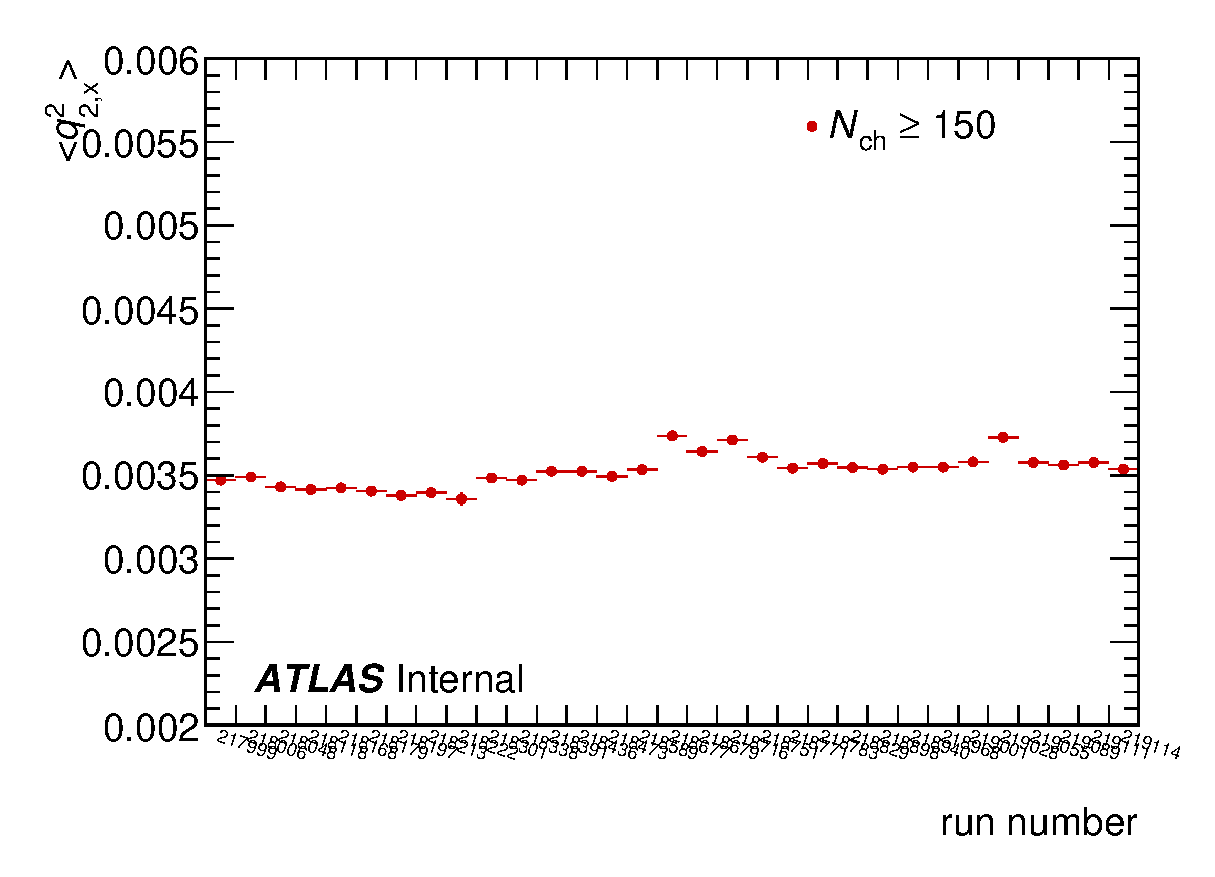
\includegraphics[width=.49\linewidth]{can_qxx.eps}
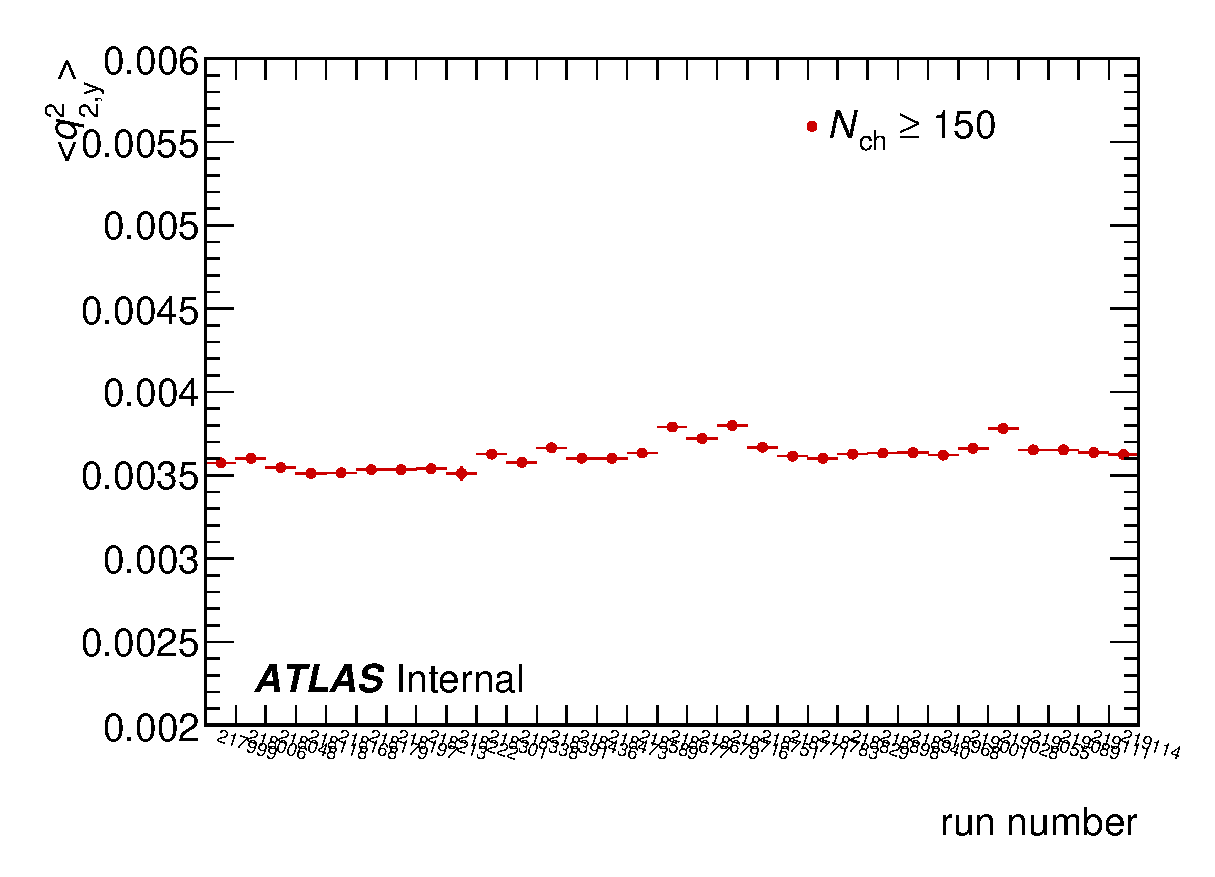
\includegraphics[width=.49\linewidth]{can_qyy.eps}\\
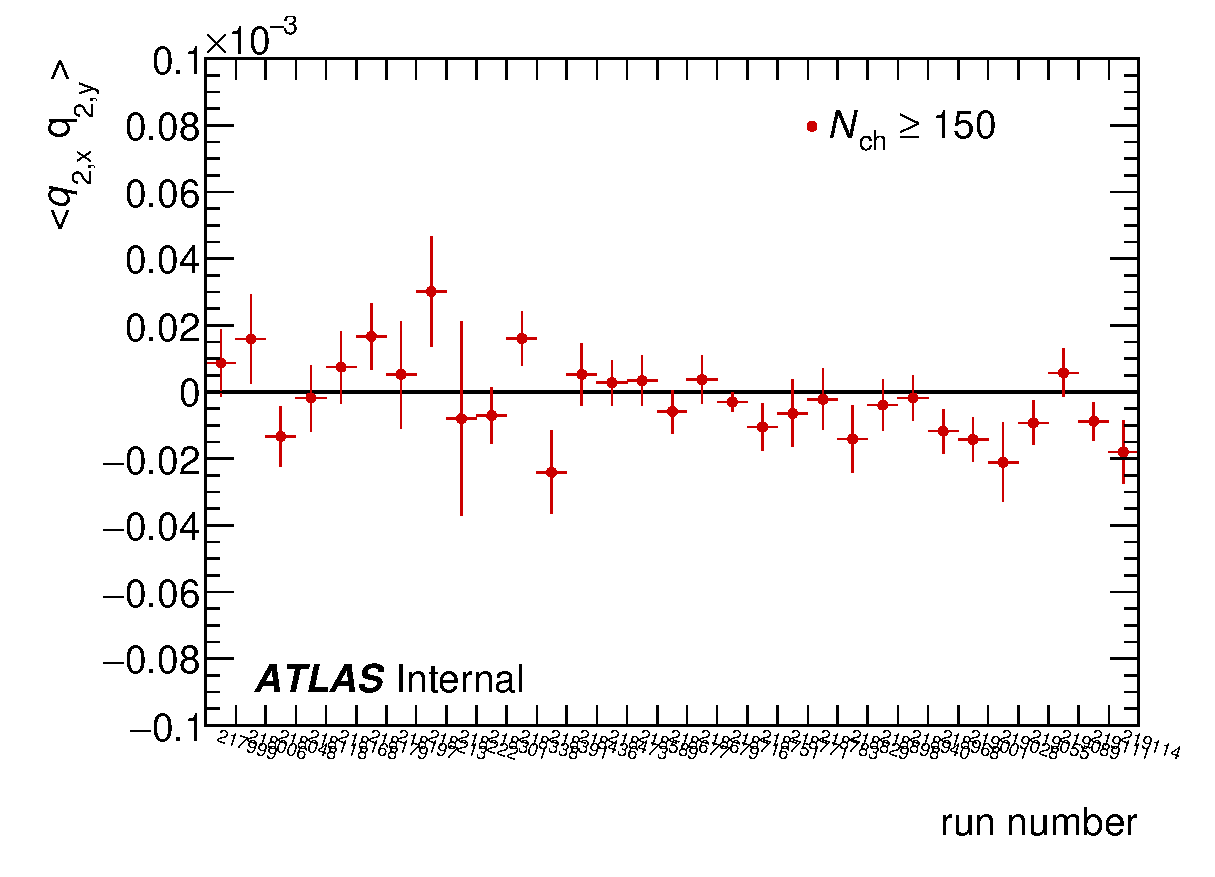
\includegraphics[width=.49\linewidth]{can_qxy.eps}
\caption{The average components of the $<\qt{}_i\ \qt{}_j>$ matrix for each run. Runs up to 218589 are from period A, and use $\eta > 2.5$, while runs after this are from period B and use $\eta < -2.5$.}
\label{fig:mean_q2_cov}
\end{figure}

As is the case for the mean subtraction correction, the correction factors are consistent over multiplicity so the events are combined for improved statistical significance in the correction.
Once these two corrections are applied run-by-run, the \psit distribution is flat (\cref{fig:dNdpsi2_corr,fig:dNdpsi2_corr_binned}).

\begin{figure}[t]
\centering
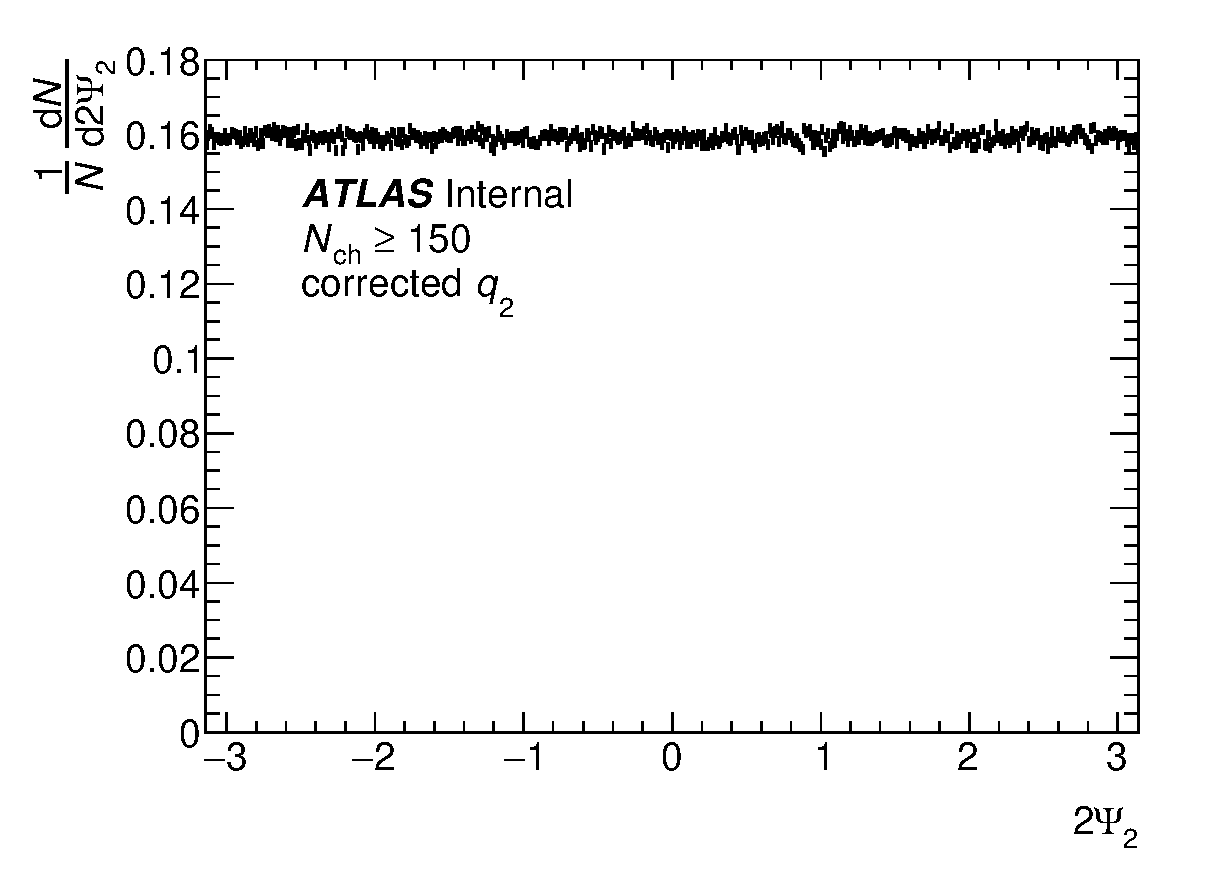
\includegraphics{dNdpsi2.eps}\\
\caption{The distribution of second-order event plane angle after first- and second-order flow vector corrections.}
\label{fig:dNdpsi2_corr}
\end{figure}

\begin{figure}[t]
\centering
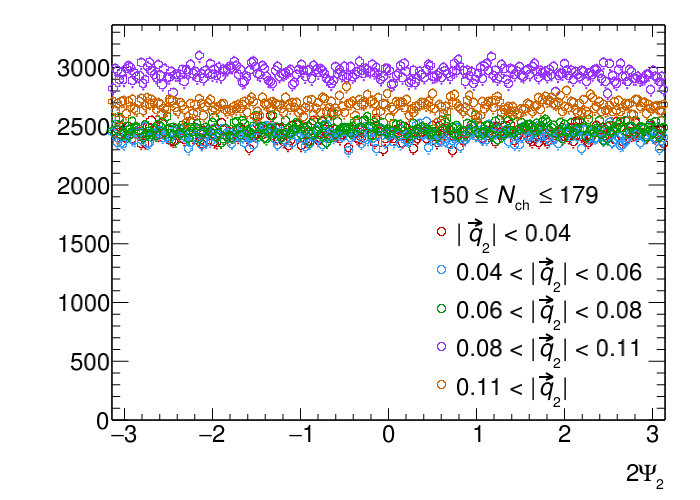
\includegraphics[width=.49\linewidth]{can_psi2_Nch150to179.png}
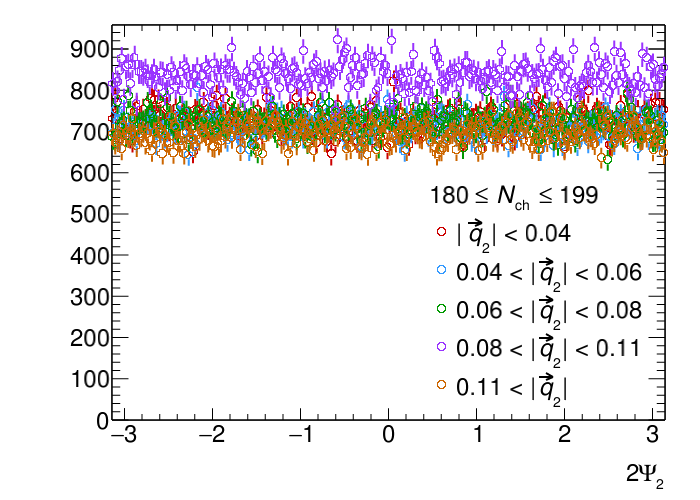
\includegraphics[width=.49\linewidth]{can_psi2_Nch180to199.png}
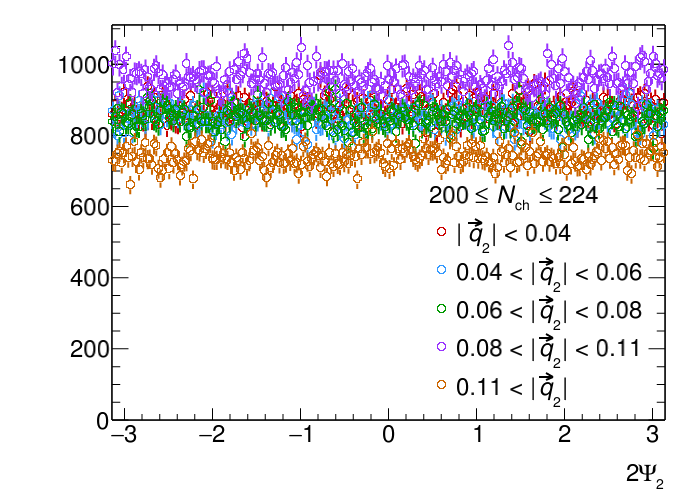
\includegraphics[width=.49\linewidth]{can_psi2_Nch200to224.png}
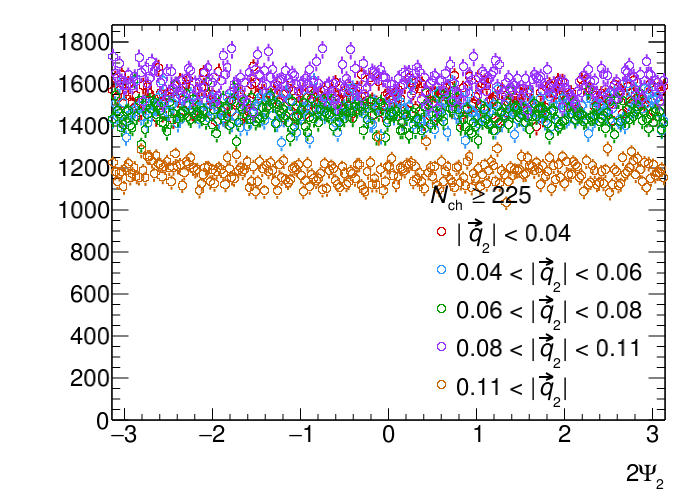
\includegraphics[width=.49\linewidth]{can_psi2_Nch225.png}
\caption{The distribution of second-order event plane angle, in bins of flow vector magnitude $|\qt|$. Each panel shows a different interval of reconstructed charged particle multiplicity \Nch.}
\label{fig:dNdpsi2_corr_binned}
\end{figure}


\subsection{Event plane angular resolution}
\label{subsec:epres}
\begin{figure}[t]
\centering
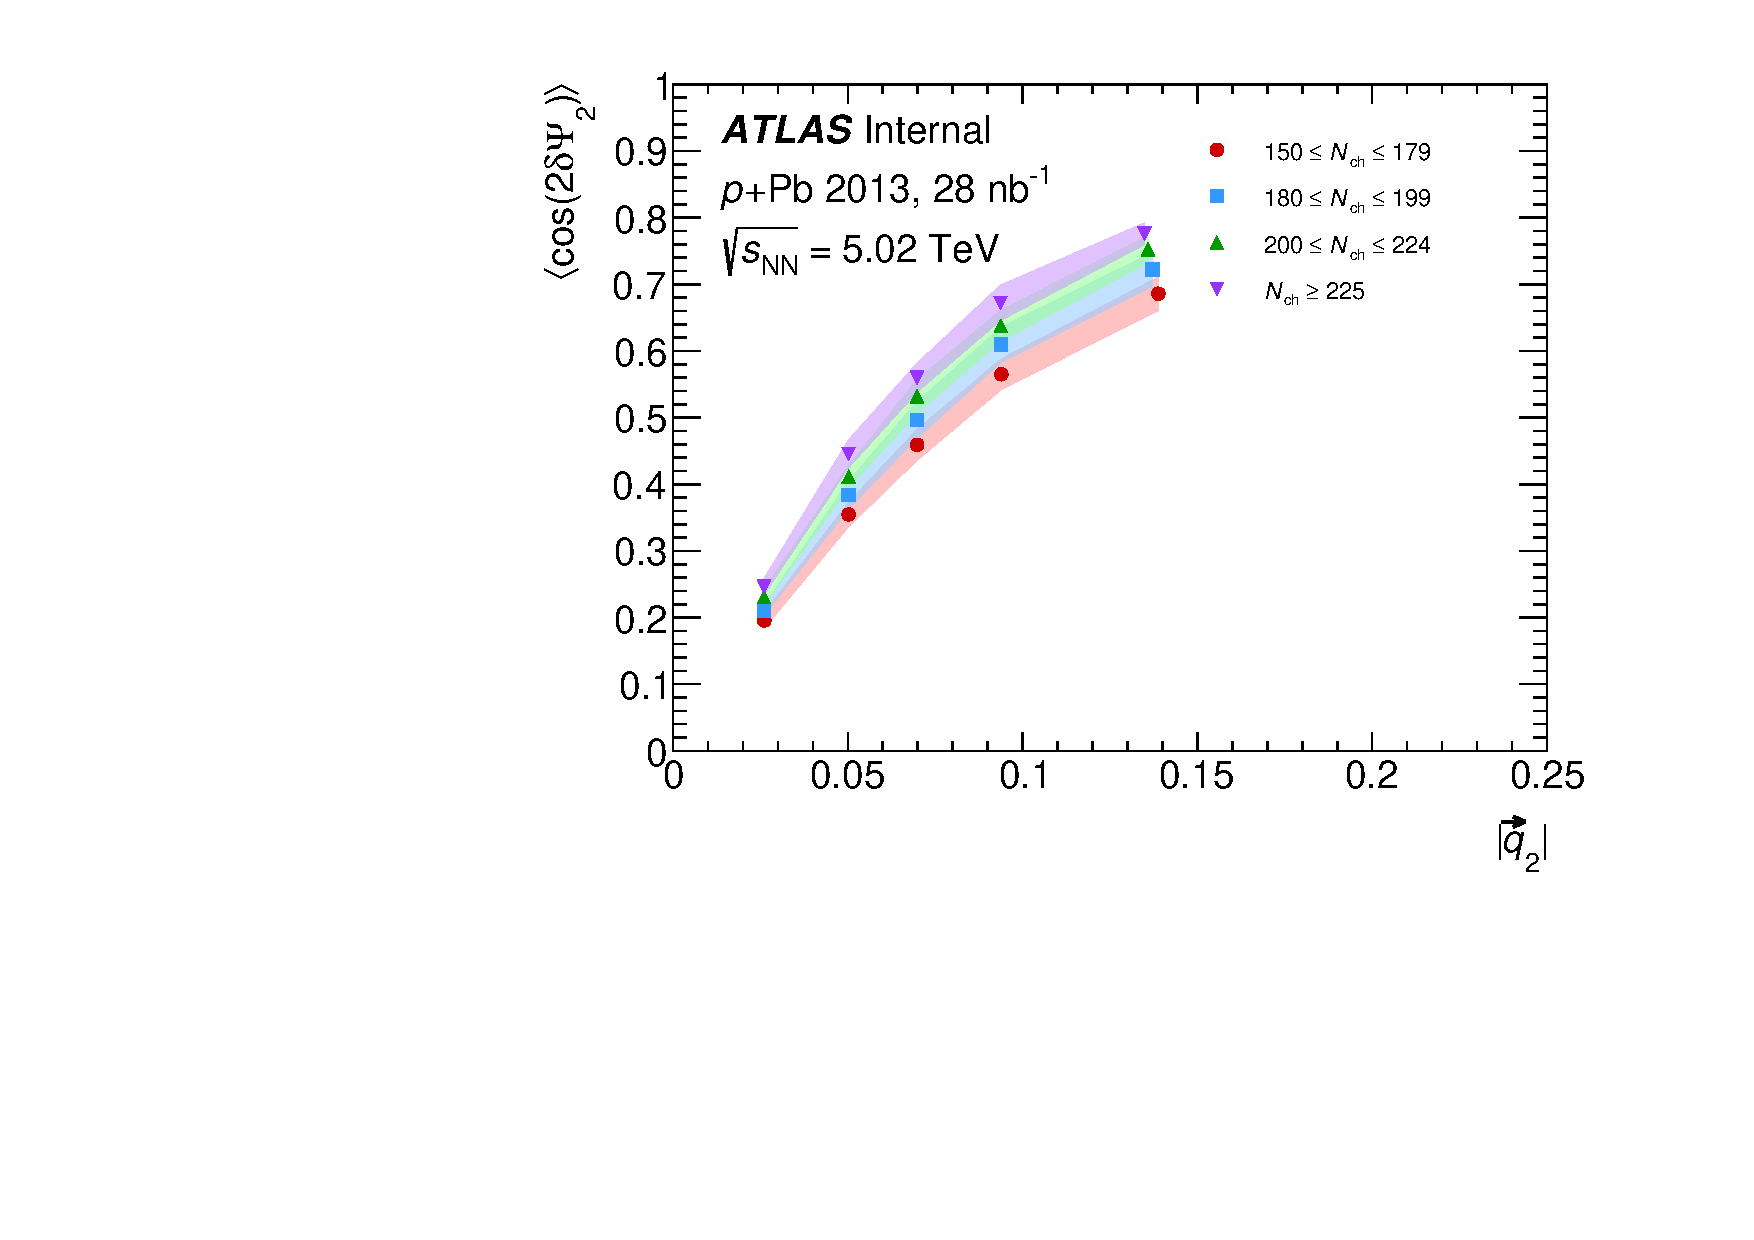
\includegraphics{epRes.pdf}\\
\caption{The event plane resolution as a function of the magnitude of the flow vector $|\qt|$ calculated using calorimeter cells with $\eta < -2.5$. Four different intervals of reconstructed track multiplicity \Nch used in the analysis are shown. The systematic uncertainties are shown in the bands, and statistical uncertainties are too small to be visible.}
\label{fig:ep_res}
\end{figure}

The event plane angular resolution, defined as $\langle \cos(2 \delta \psit) \rangle$ where $\delta \psit$ is the difference between true and measured \psit, is shown in \cref{fig:ep_res} measured with the calorimeters in the lead-going direction at $\eta < -2.5$.
The resolution is shown separately for periods A and B, but since they are comparable only the combined resolution is used.
This quantity can be calculated from data using the three-sub-event method, where two other subdetectors are chosen with rapidity ranges $-2 < \eta< -0.5$ and $0 < \eta < 1.5$.
In this expression each subevent is defined by pseudorapidity ranges with a pseudorapidity gap of 0.5 left in between each subdetector so that biases are not introduced from jets overlapping two subdetectors.
The event plane resolution of the nominal subdetector can be calculated with the following expression.
\begin{equation}
\langle \cos(2 \delta \psit) \rangle = \sqrt{ \frac{\langle \cos(2\psit^A - 2\psit) \rangle \langle \cos(2\psit^B - 2\psit) \rangle }{\langle \cos(2\psit^A - 2\psit^B) \rangle} }\\
\end{equation}
Here $\psit^A$ refers to the event plane measured using calorimeters with $-2 < \eta< -0.5$ and $\psit^B$ refers to that with $0 < \eta < 1.5$.
Each of these additional subevents has first- and second-order corrections applied that are derived for each region of the detector in the same way that the corrections are derived for the nominal subdetector with $\eta < -2.5$.
Systematic uncertainties in the event plane resolution are taken from two sources.
The alternate subdetectors are shifted by $\Delta\eta = +0.5$ and the difference in the event plane resolution is symmetrized.
Also, the alternate subdetectors are calculated using the \qt from tracks weighted by their \pt.
This difference is also symmetrized, and these two contributions are added in quadrature.


\FloatBarrier
\section{Correlation function}
\label{sec:corr_func}
The two-particle correlation function is defined as the ratio of two-particle to single-particle momentum spectra:
\begin{equation} \label{eq:corr_deff}
  %% ; \kt, \kys, \kphi
  C\left(\mathbf{p}^a, \mathbf{p}^b\right) \equiv \dfrac{\left(\dfrac{dN^{ab}}{d^3\mathbf{p}^a \, d^3\mathbf{p}^b}\right)}{\left(\dfrac{dN^{a}}{d^3\mathbf{p}^a}\right)\left(\dfrac{dN^{b}}{d^3\mathbf{p}^b}\right)} \,,
\end{equation}
for pairs of particles with momenta $\mathbf{p}^a$ and $\mathbf{p}^b$.
The correlation function is expressed as a function of the relative momentum $\mathbf{q} \equiv \mathbf{p}^a - \mathbf{p}^b$ in intervals of the transverse component \kt of the average momentum $\mathbf{k} \equiv \left(\mathbf{p}^a + \mathbf{p}^b\right)/2$.
The correlation function is measured in intervals of transverse pair momentum \kt and either the rapidity \kys or the azimuthal angle of the pair with respect to the second-order event plane, $\kphi-\psit$.
Because the second-order event plane angle is two-fold degenerate, the observables are invariant under an azimuthal rotation $\kphi \rightarrow \kphi + \pi$, and can be expressed without loss of generality as functions of $\tdpk$. %% \equiv 2(\kphi-\psit)$. %% come up with other notation?
The kinematic variables for the azimuthal analysis are shown in a transverse projection in \Fig{\ref{fig:transverse_q}}.

\begin{figure}[t]
  \centering
  \includegraphics{transverse_q.png}
  \caption{A transverse projection of the kinematic variables of a track pair with respect to the event plane.}
\label{fig:transverse_q}
\end{figure}

The numerator and denominator of \Eqn{\ref{eq:corr_deff}} are expressed in terms of the variables of interest with the following notation:
\begin{align}
  A\left[\mathbf{q};\kt, \kys, \tdpk\right] &\equiv \left. dN_\textrm{pair}/d^3 \mathbf{q} \right|_{\textrm{same}} \\
  B\left[\mathbf{q};\kt, \kys, \tdpk\right] &\equiv \left. dN_\textrm{pair}/d^3 \mathbf{q} \right|_{\textrm{diff}}
\end{align}
where $A(\mathbf{q})$ is a histogram formed with pairs from the same event in each event class and $B(\mathbf{q})$ is a histogram formed with pairs that do not have correlations from being in the same event but are also each drawn from the same event class.
The combinatorial background $B(q) \equiv \left. dN/dq \right|_{\textrm{diff}}$ is constructed either by event mixing or, for the azimuthal analysis, by the pair sampling procedure.
Each of these approaches will be described below.
The ratio of the distributions defines the correlation function:
\begin{equation}
  \label{eq:same_over_mixed}
  C\left[q;\kt, \kys, \tdpk\right] \equiv \frac{A_{\mathbf{k}}(q)}{B_{\mathbf{k}}(q)}
\end{equation}
which in practice is a function either of \kys or \tdpk, not both.

\subsection{Track pair cuts}
All particle pairs are required to have $\left| \Delta \phi \right| < \pi/2$.
Without this cut an enhancement is observed at large relative momentum from di-jets.
While the physics of interest happens at low relative momentum, an enhancement at large relative momentum can affect the asymptotic normalization of the fit functions, which can in turn impact the quality of the fit.

Opposite-sign pairs are rejected if their $\sqrt{s}$ is near one of a few known resonances.
In calculating the invariant mass of each pair, the track masses are assumed to be one of the sets of possible daughter particles (in this case $\pi^{\pm}$ or $K^{\pm}$).
The pair is rejected if their invariant mass is within $20~\MeV$ of the mass of the possible parent particle, except in the case of the $\rho^{0}$, where pairs are rejected if they are within 2 half-widths of $m_{\rho^{0}}$, at $626.2 \MeV < \sqrt{s} < 924.4 \MeV$.
The decays rejected are the following:
\begin{itemize}
\item
  $\rho^{0} \rightarrow \pi^{+} \pi^{-}$
\item
  $K^{0}_{S} \rightarrow \pi^{+} \pi^{-}$
\item
  $\phi(1020) \rightarrow K^{+} K^{-}$
\end{itemize}

\subsection{Event mixing}
\label{subsec:evt_mixing}
The event-mixed background $B(q) \equiv \left. dN/dq \right|_{\textrm{mix}}$ is constructed by selecting one particle from each of two events in the same event class as $A(q)$.
This approach has the useful property that most single-particle efficiency, acceptance, and resolution effects cancel in the ratio.
This event mixing approach is therefore used when possible except in the azimuthally-dependent analysis where it is precluded by the event plane resolution correction.

Each particle in the background satisfies the same selection requirements as those used in the same-event distribution.
Event classes are categorized by centrality so that events are only compared to others with similar multiplicities and momentum distributions.
Events are also sorted by the longitudinal position of the primary vertex $z_\textrm{PV}$ so that the background distribution is constructed with pairs of tracks originating from nearby space points, which is necessary for $B(q)$ to accurately represent the as-installed detector.
The $A(q)$ and $B(q)$ distributions are combined over $z_\textrm{PV}$ intervals in such a way that each of them represents the same $z_\textrm{PV}$ distribution.

\subsection{Event plane resolution correction}
\label{subsec:epres_corr}
The event plane resolution has the effect of reducing the second-order Fourier components of event-by-event observables.
For instance, given true and measured event plane angles $\psit^\textrm{tr}$ and $\psit^\textrm{m}$ with $\psit^\textrm{m} = \psit^\textrm{tr} + \delta\psit$, the relevant Fourier components of an azimuthally-dependent observable $\mathcal{O}$ are
\begin{equation}
  \begin{split}
    \mathcal{O}^\textrm{m} \left[2(\phi-\psit^\textrm{m})\right] =& \mathcal{O}_\textrm{,0} + \mathcal{O}_\textrm{,c2} \cos\left[2(\phi - \psit^\textrm{m})\right]
    + \mathcal{O}_\textrm{,s2} \sin\left[2(\phi - \psit^\textrm{m})\right]\\
    =& \mathcal{O}_\textrm{,0} + \mathcal{O}_\textrm{,c2} \cos\left[2(\phi - \psit^\textrm{tr} - \delta\psit)\right]
    + \mathcal{O}_\textrm{,s2} \sin\left[2(\phi - \psit^\textrm{tr} - \delta\psit)\right]\\
    =& \mathcal{O}_\textrm{,0} + \left\{\mathcal{O}_\textrm{,c2} \cos\left[2(\phi - \psit^\textrm{tr})\right]
    + \mathcal{O}_\textrm{,s2} \sin\left[2(\phi - \psit^\textrm{tr})\right]\right\} \cos(2\delta\psit)
  \end{split}
\end{equation}
where $\mathcal{O}_\textrm{,0}$ is the 0th-order Fourier component and $\mathcal{O}_\textrm{,c2}$ and $\mathcal{O}_\textrm{,s2}$ are the 2nd-order cosine and sine Fourier components, respectively.
Therefore, over many events the event plane resolution effectively reduces the 2nd-order Fourier components of an observable by a factor of $\langle \cos\left(2\delta\psit\right) \rangle$.
A correction is performed on the same-event distribution $A$, as described in \Ref{\cite{Heinz:2002au}}, to compensate for this effect as well as the effect of non-infinitesimal azimuthal bin widths:
\begin{equation}
  \label{eq:a_corr}
  A^\textrm{corr}[q,\tdpk] = A^\textrm{exp}(q) + 2\xi \left\{ A_\textrm{,c2}(q) \cos\left[\tdpk\right] + A_\textrm{,s2}(q) \sin\left[\tdpk\right] \right\}
\end{equation}
where
\begin{align}
  \xi =& \frac{\pi/N_\textrm{bins}}{\langle \cos\left(2\delta\psit\right) \rangle \sin\left(\pi/N_\textrm{bins}\right)} - 1 \label{eq:xi_def} \\
  A_{,\textrm{c}2}(q) =& \frac{1}{N_\textrm{bins}} \sum_{i=1}^{N_\textrm{bins}} A^\textrm{exp}\left[q,\tdpk_i \right] \cos \left[ \tdpk_i \right] \\ 
  A_{,\textrm{s}2}(q) =& \frac{1}{N_\textrm{bins}} \sum_{i=1}^{N_\textrm{bins}} A^\textrm{exp}\left[q,\tdpk_i \right] \sin \left[ \tdpk_i \right]
\end{align}
and $\Nbins = 8$ is the number of azimuthal bins.
Only the 2nd harmonic is corrected in this procedure. Higher-order harmonics, while potentially of physical interest, are more difficult to measure and are not considered in this analysis.

The combinatoric background $B(q) \equiv \left. dN/dq \right|_{\textrm{mix}}$ is traditionally constructed by event mixing, that is, by selecting one particle from each of two events in the same event class as $A(q)$ as described in \cref{subsec:evt_mixing}.
However, with an azimuthally-differential analysis the event plane resolution correction precludes event mixing because there is no simple decomposition of a mixed-event distribution into its Fourier components (as there are two independent event plane in each event pair).
Previous azimuthal femtoscopic measurements have corrected the mixed-event distribution $B$ in the same way that the same-event distribution $A$ is corrected, as suggested in \Ref{\cite{Heinz:2002au}}.
However, this fails to account for the fact that the independent smearing of the two event planes changes the shape of the pair distribution, and when projected into $q$-space it cannot be simply corrected bin-by-bin.

On the other hand it is possible to correct the single-particle momentum distribution in the same way as \cref{eq:a_corr}.
The dependent variables are \pt and $\eta$ instead of $\mathbf{q}$, and there are many more azimuthal bins (in \Eqn{\ref{eq:xi_def}} the $N_\textrm{bins} = 64$ of $2(\phi - \psit)$ as opposed to 8 bins of $2(\kphi - \psit)$), but the procedure is otherwise identical.
Pairs of momentum are then sampled from this corrected distribution as discussed in detail in \cref{subsec:bkgd_sampling}.

The correlation function $C(q)$ is then formed by taking the ratio of the corrected same- and mixed-event relative momentum distributions
\begin{equation}
  C(q) = \frac{A^\textrm{corr}(q)}{B^\textrm{corr}(q)}
\end{equation}
where $B^\textrm{corr}$ is generated by sampling pairs from $N^\textrm{corr}$, as described in the following sections.

\subsection{Pair sampling}
\label{subsec:bkgd_sampling}
The single-particle distribution can be corrected for the event plane resolution, following the procedure for the pair distribution.
It is not possible to correct the mixed-event pair distributions properly, at least not without extending the analysis in an additional dimension (\psit) which would require an infeasible amount of memory and CPU resources.
Pairs can be sampled from the single-particle distribution after it is corrected.
Building a background with sampling is usually not as precise as mixed-event distributions, but in an azimuthal analysis the event plane resolution correction is a dominant effect, so it is necessary to structure the measurement around it.

The sampling method does not account exactly for variations of the detector acceptance and efficiency over \pt, $\eta$, and \kphi, because each track contributes a count to a bin which represents a small range of possible values of \pt, $\eta$, and \tdpk.
The sampled background pair distribution $B(q)$ is multiplied by the ratio of an event-mixed distribution to a sampled pair distribution (\cref{fig:sample_to_mix_ratio}) in order to compensate for the effect of the sampling procedure.
Both distributions in this ratio are not corrected for event plane resolution, since such a correction cannot be applied to the mixed-event pair distribution.
At small relative momentum, where the \ac{HBT} signal is relevant, there is no significant effect from the sampling.
This multiplicative correction is applied as a function of \kt.

It is prohibitive statistically and/or computationally to bin the analysis in \psit as well as \tdpk, which would require increasing the size of the analysis by about a factor of 64.
As a result, the sampled momentum $\mathbf{p}$ distribution does not fully account for azimuthal anisotropies in the pair response of the detector.
This effect is described by the ratio of a distribution of mixed events to a similar distribution in which one of the events is smeared by a random angle (\cref{fig:phi_corr_to_uncorr_ratio}).
The background is multiplied by this ratio, which is evaluated as a function of \kt.

\begin{figure}[t]
\centering
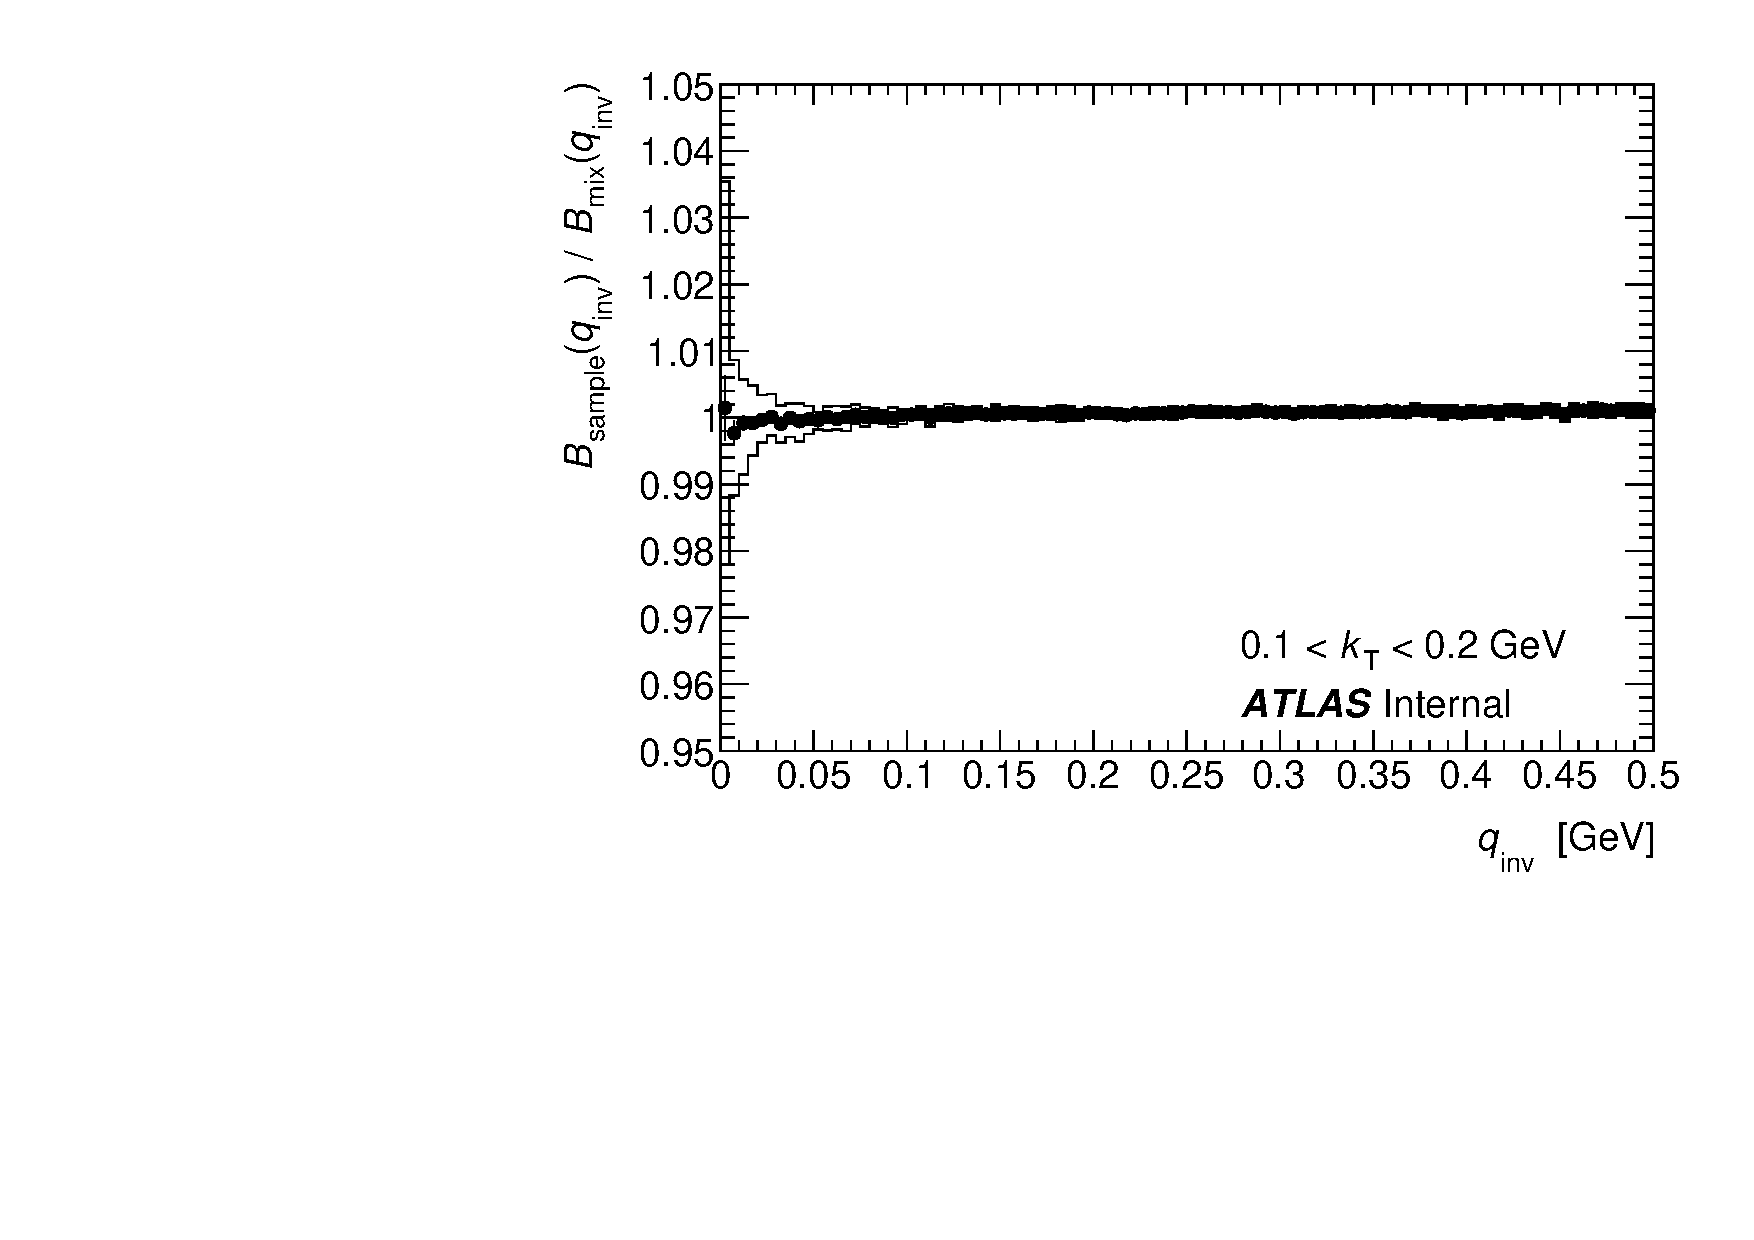
\includegraphics[width=.49\linewidth]{sample_to_mix_ratio_kt0.pdf}
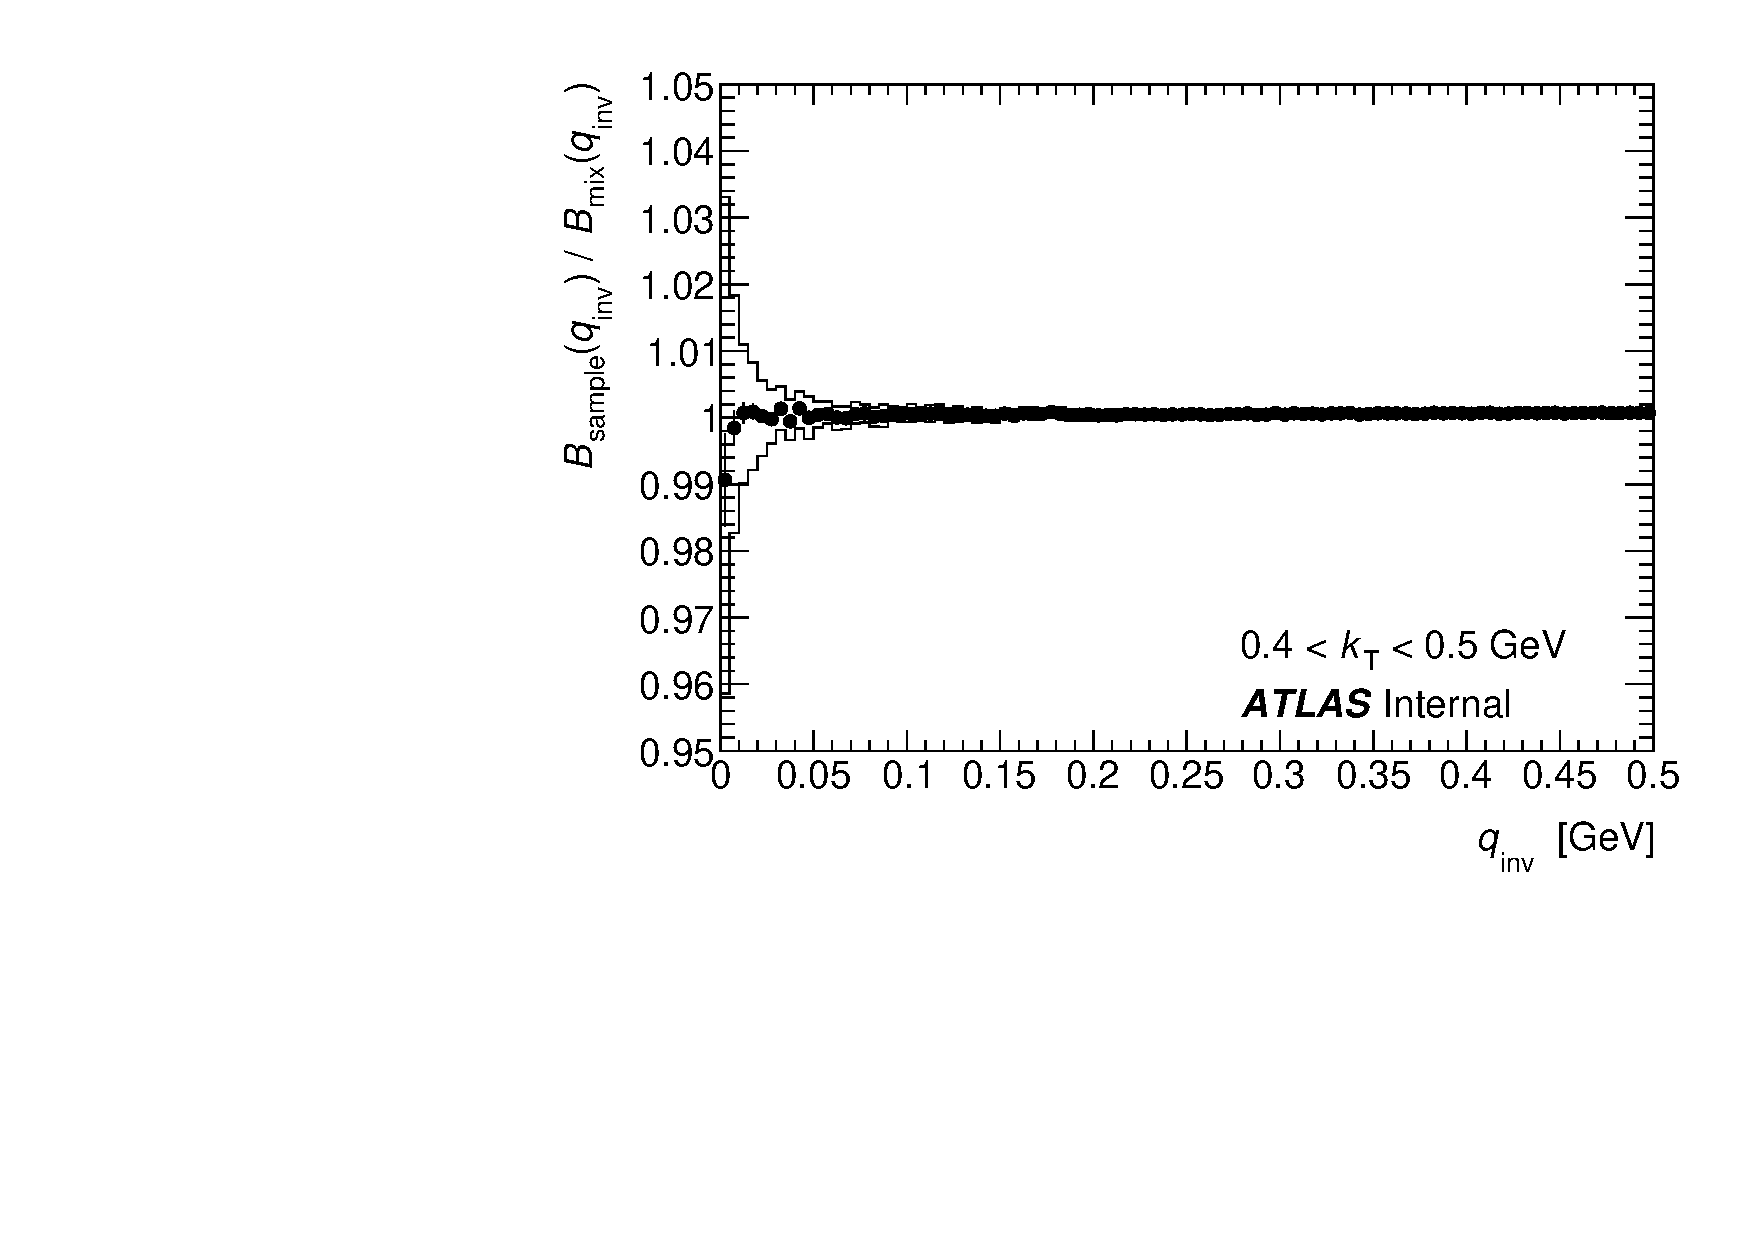
\includegraphics[width=.49\linewidth]{sample_to_mix_ratio_kt3.pdf}\\
\caption{The ratio of a sampled distribution to an event-mixed distribution, both of which are not corrected for event plane resolution. This shows the effect of sampling from a finite number of bins. The central points are shown as circles with statistical uncertainties and the bands indicate the systematic uncertainty, which is discussed in \cref{sec:systematics}.}
\label{fig:sample_to_mix_ratio}
\end{figure}

\begin{figure}[t]
\centering
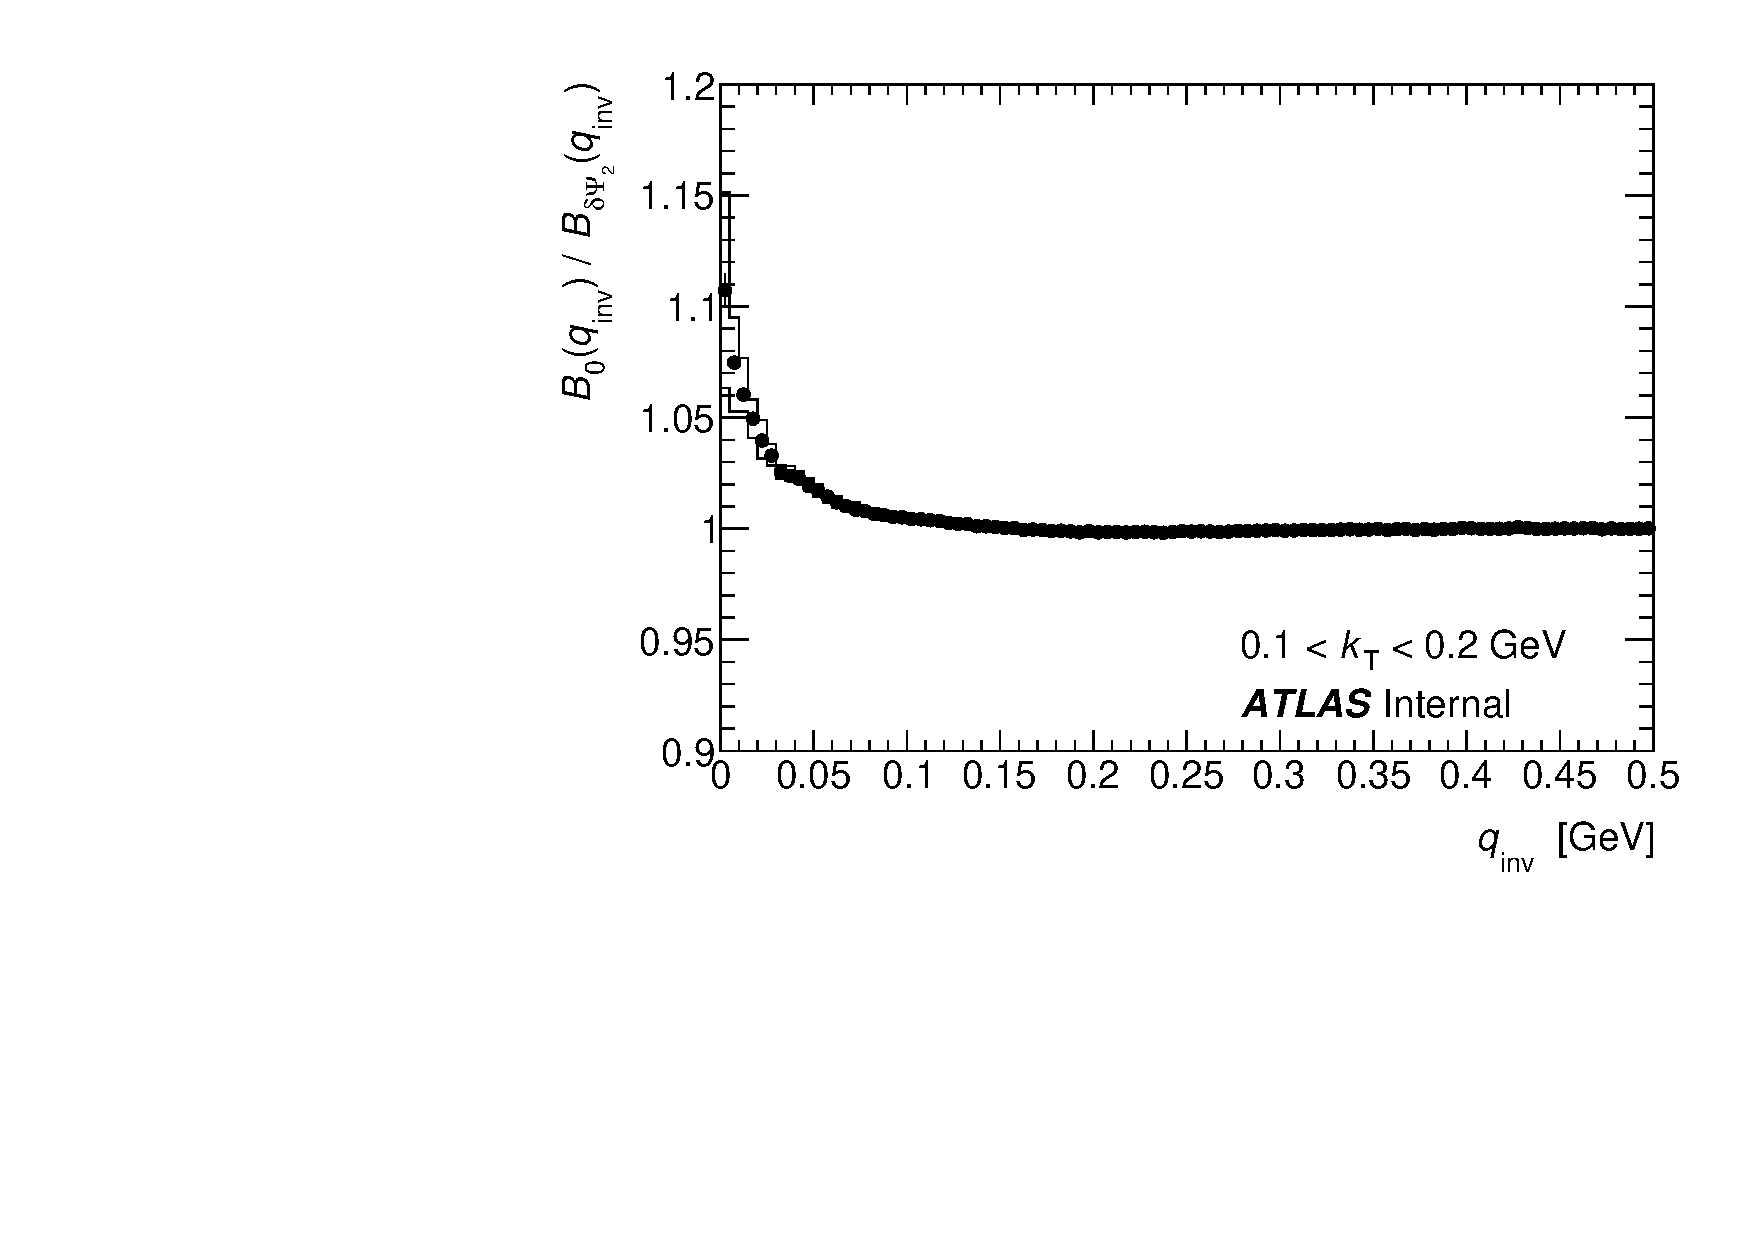
\includegraphics[width=.49\linewidth]{phi_corr_to_uncorr_ratio_kt0.pdf}
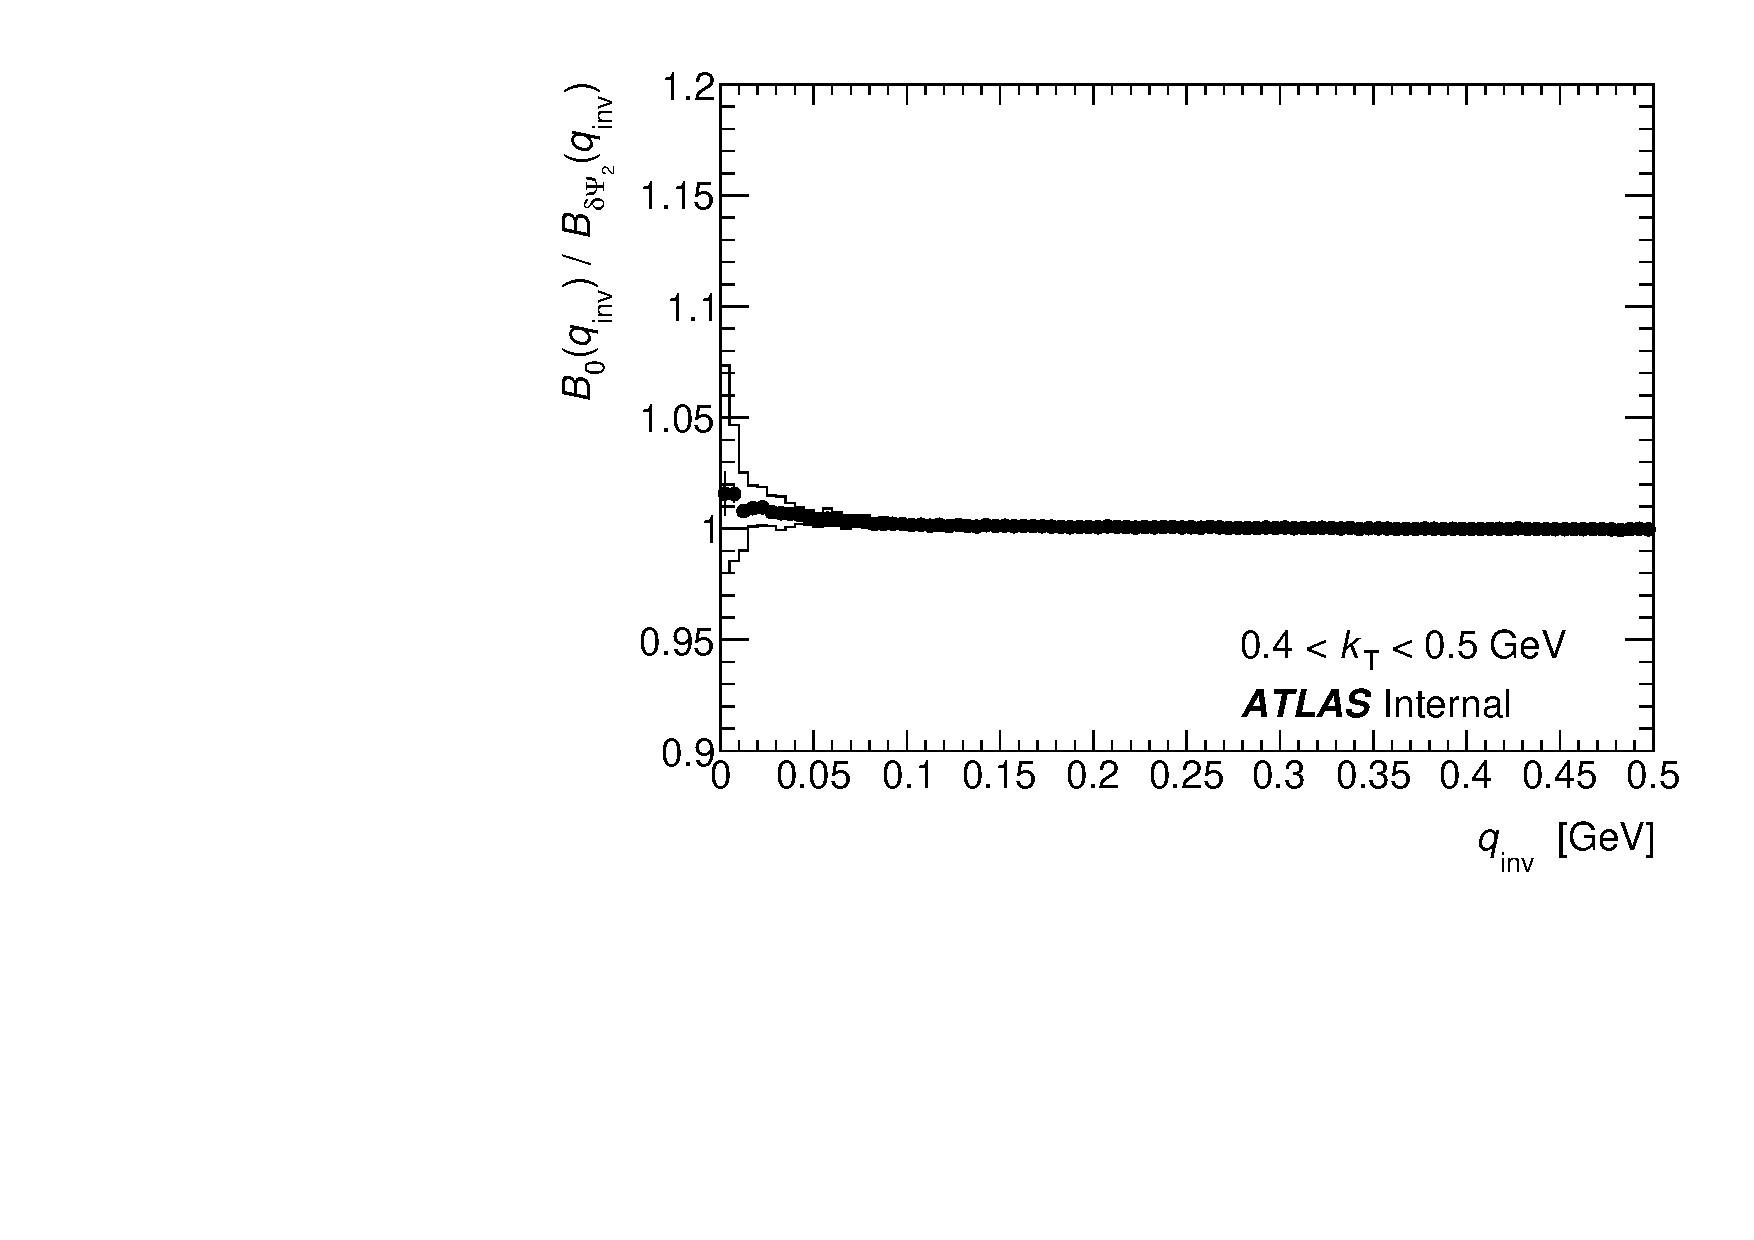
\includegraphics[width=.49\linewidth]{phi_corr_to_uncorr_ratio_kt3.pdf}\\
\caption{The ratio of an event-mixed distribution to an event-mixed distribution with randomized azimuthal angle between the events. This demonstrates the effect of not binning events in \psit. The central points are shown as circles with statistical uncertainties and the bands indicate the systematic uncertainty, which is discussed in \cref{sec:systematics}.}
\label{fig:phi_corr_to_uncorr_ratio}
\end{figure}

The single-particle experimental distribution $N^\mathrm{exp}[\pt, \eta, \tdpp]$ is corrected similarly to the pair distribution $A(q)$ in \cref{eq:a_corr}, however it is also explicitly symmetrized in $\phi$ so there is no sine term added.
\begin{equation}
  \label{eq:n_corr}
  N^\textrm{corr}[\pt, \eta, \tdpp] = N^\textrm{exp}_\textrm{symm}\left[\pt, \eta, \tdpp\right] + 2\xi N_\textrm{,c2}(\pt, \eta) \cos\left[\tdpp\right]
\end{equation}
where
\begin{equation}
N^\textrm{exp}_\textrm{symm}\left[\pt, \eta, \tdpp\right] \equiv \frac{N^\textrm{exp}[\pt, \eta, \tdpp] + N^\textrm{exp}[\pt, \eta, -\tdpp]}{2}  \; .
\end{equation}
Without the explicit symmetrization, fluctuations in the azimuthally-odd part of the distribution can lead to nonphysical sine terms in the sampled background. %% Note that there is no detector effect to consider here: the event plane \psit is effectively integrated over. Detector effects not accounted for as a result of this are considered in a systematic uncertainty.

Events are grouped by run period, $z_\textrm{vtx}$, charged-particle multiplicity \Nch (with $\pt > 400$ \MeV), and flow vector magnitude $|\qt|$, for a total number of classes of $2 \times 40 \times 4 \times 5 = 1600$.
The events are combined within each run period, so that the 15 runs from period A and the 16 runs from period B are combined.
This is necessary to sufficiently populate the single-particle distributions to minimize auto-correlations.
Because the 3D momentum histograms need to be densely populated, a large number of events are needed even when each event has a large multiplicity.
The number of events in each of these event classes is shown in \cref{fig:evt_class}.
Each event class has a minimum of 100 events, but most have greater than 1000.

\begin{figure}[t]
\centering
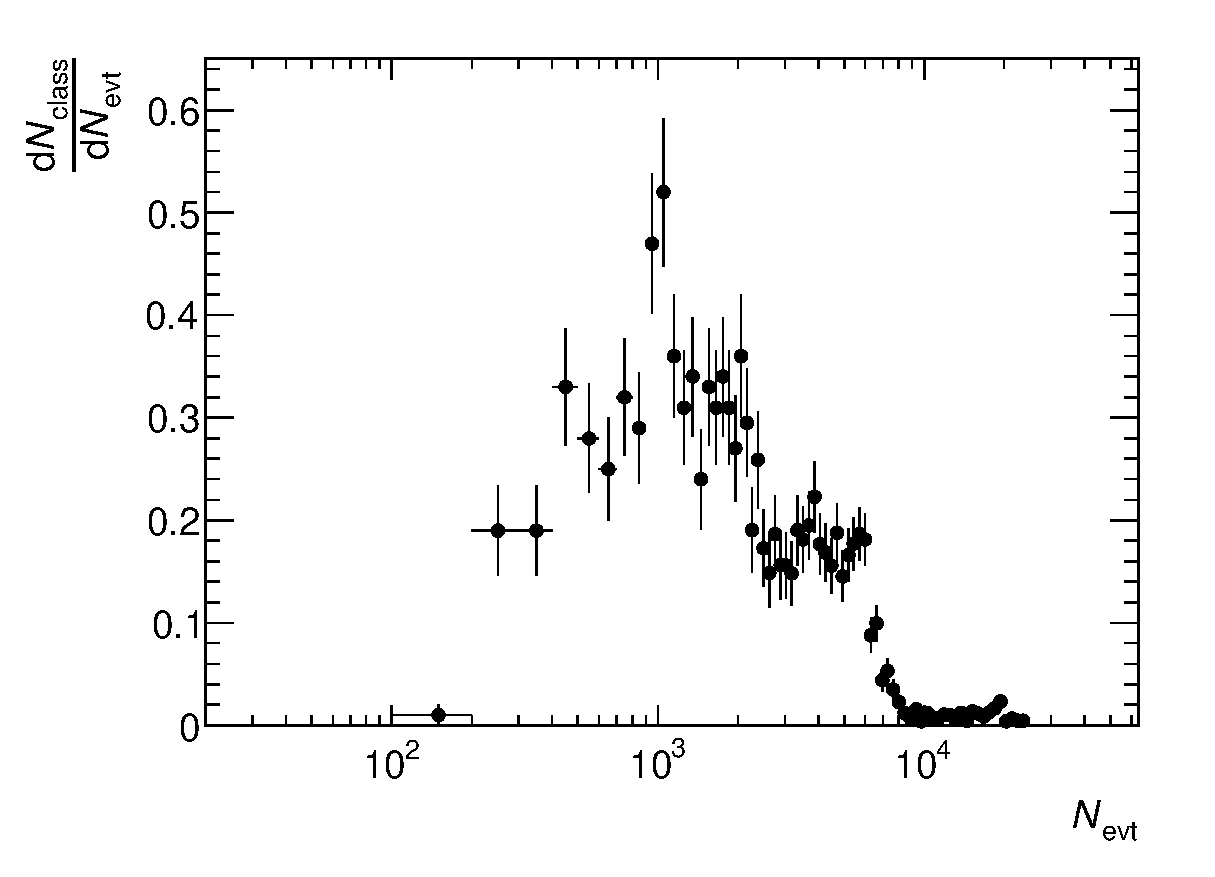
\includegraphics{evt_class.eps}\\
\caption{Differential probability distribution of the number of event classes having a given number of events, where the event class is determined by run period, $z_\textrm{vtx}$, multiplicity, and flow vector magnitude $|\qt|$. The distribution is normalized to unity.}
\label{fig:evt_class}
\end{figure}

Within each event class, tracks are sampled from the histogram of the single-particle distribution $N \left[ \pt, \eta, 2(\phi-\psit) \right] $.
A pre-processing step is performed to surjectively assign each bin of the 3D histogram an interval in $(0,1)$ with size proportional to the bin content, representing the cumulative distribution function (CDF) of the histogram distribution at each bin edge.
For each new track a random number is generated in the uniform distribution $U(0,1)$, and a bin is selected by binary search according to the assignment from the pre-processing step.
The values of the three kinematic variables are set by generating uniform random variables from a range of each of the corresponding bin edges.
One of these three random number generations is optimized away, because given that a bin has been selected by the initial random number, that number has a distribution $U(a, b)$ where $a$ and $b$ are the endpoints of its CDF interval.
It can then be scaled linearly to lie between the bin edges of the relevant kinematic variable.
%% with a linear scaling of the value of the initial uniform random number relative to the endpoints of the histogram bin's CDF interval. %% paragraph break?

When pairs tracks are drawn from the same distribution (i.e. same-charge particles in an event class), an additional step is taken to simulate sampling without replacement.
If the second track is randomly drawn from the same bin as the first track, the process continues as normal only with probability $\frac{N_\textrm{bin count} - 1}{N_\textrm{bin count}}$.
In other words, the bin is rejected with probability $1/N_\textrm{bin count}$.
Otherwise the bin is disallowed for the second particle, and its bin is redrawn until it corresponds to a different bin than the first particle's.
Without this correction for sampling-without-replacement, there is a small but significant enhancement at low $|\mathbf{q}|$ of the sampled pair distribution relative to the classically event-mixed distribution.

\begin{figure}[t]
\centering
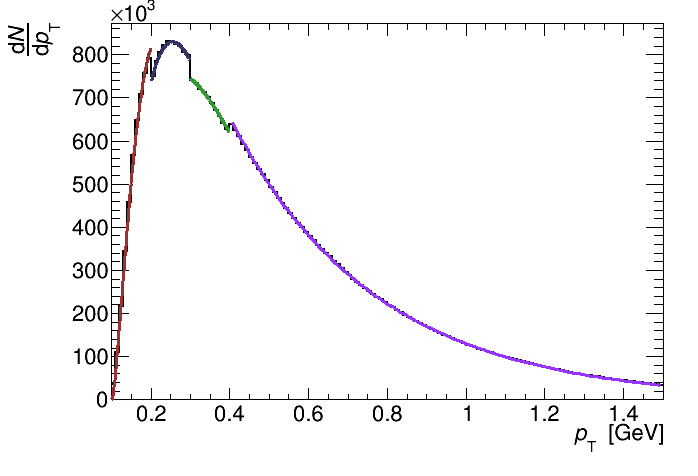
\includegraphics[width=.49\linewidth]{pos_pt.png}
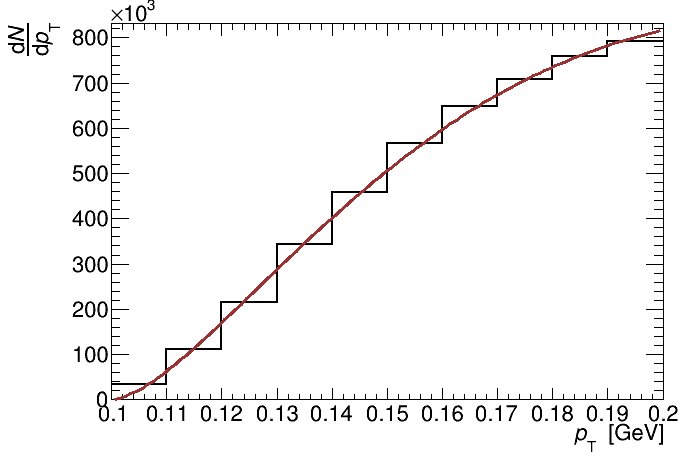
\includegraphics[width=.49\linewidth]{pos_pt_zoom_bin.png}\\
\caption{The \pt spectrum for positive tracks (left), and a zoomed view of the low-\pt region (right). Each segment is fit to a gamma distribution with variable location which represents the smooth spectrum. The segments are determined by edges at 100, 200, 300, and 400 \MeV, where there are jumps in SCT hit requirements or a turn-on of TRT seeding (at 400 \MeV).}
\label{fig:pt_fits}
\end{figure}

\FloatBarrier

The physical \pt distribution has a steep slope in many places, and the detector response is relatively smooth as a function of \pt.
By contrast, the sampled distribution from the histogram of the single-particle distribution will have sharp jumps at bin edges, so where the slope is large the value of the sampling distribution can be far from that of a smooth one near a bin edge, as illustrated in \cref{fig:pt_fits}.
A correction procedure is applied to remove these sharp edges in the \pt profile of the sampled distribution. In each event class, the \pt distribution is fit to a 4-parameter gamma distribution in four intervals (with boundaries corresponding to changes in the \sct hit requirements).
A first-order correction is performed to transform the random \pt value to another one in the same bin, to account for the slope of the probability distribution in that bin.
The slope used for this procedure is that computed from the fit function in the \pt interval.
The adjusted \pt is given by
\begin{equation}
  \pt \rightarrow \pt + \frac{f'}{2} (b-a) (\pt-a) (b-\pt)
\end{equation}
where the bin edges of the \pt bin are $a$ and $b$ and the approximate numeric derivative of the probability distribution is $f'$.
The result of this process is illustrated in \cref{fig:sample_slope_corr} on a toy distribution.
Samples are drawn from a coarse-binned distribution, and the distribution of the modified random variable accounts for the underlying slope.

\begin{figure}[t]
\centering
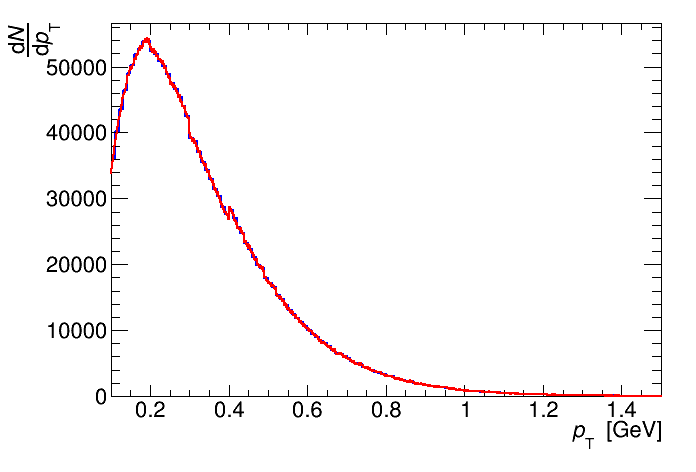
\includegraphics[width=.49\linewidth]{testMomHistSampler.png}
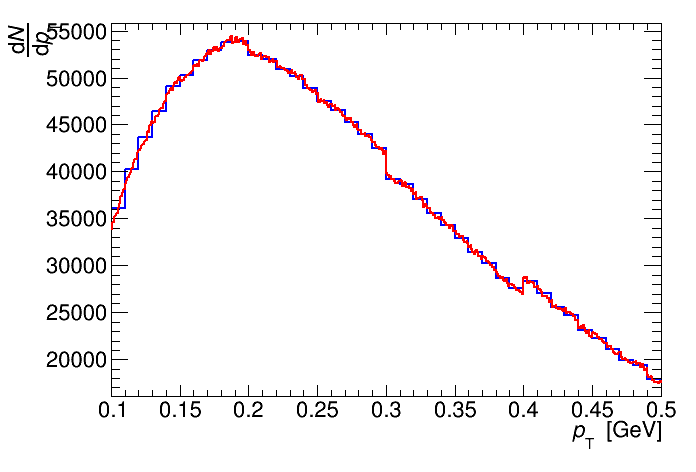
\includegraphics[width=.49\linewidth]{testMomHistSamplerZoom.png}\\
\caption{An illustration of the effects of the \pt slope correction on the sampled momentum distribution. The course-binned histogram is used to generate samples for the fine-binned histogram.}
\label{fig:sample_slope_corr}
\end{figure}


\subsection{Parameterization of the correlation function}

The Bose-Einstein enhancement in the invariant correlation functions is fit to an exponential form:
\begin{equation} C_{\textrm{BE}}(\qinv) = 1 + \mathrm{e}^{- \Rinv \qinv } \,, \label{eq:cbe_qinv}\end{equation}
where \Rinv is the Lorentz-invariant \ac{HBT} radius. This function corresponds to an underlying Breit-Wigner source density.

The Bose-Einstein component of the three-dimensional correlation functions is fit to a function of the form
\begin{equation}
C_{\textrm{BE}}(\mathbf{q}) = 1 + \mathrm{e}^{- \left\| R \mathbf{q} \right\|} \;, \label{eq:cbe_qosl}
\end{equation}
where $R$ is the symmetric matrix in \cref{eq:r_matrix_full}.

The full form of the invariant-correlation-function fit to like-charge track pair data including the hard-process background description is
\begin{equation}
C(q) = \mathcal{N} \left[1-\lambda + \lambda K(\qinv)C_{\textrm{BE}}(q)\right] \Omega(q) \,,\label{eq:correlation_function_full}
\end{equation}
where $\mathcal{N}$ is a normalization factor, $C_\mathrm{BE}(q)$ is given by \cref{eq:cbe_qinv} or \cref{eq:cbe_qosl}, the Coulomb correction $K(\qinv)$ is discussed in \cref{subsec:coulomb}, and the hard process background $\Omega(q)$ is discussed in detail in \cref{sec:jet_frag}.
When opposite-charge pairs are fit to constrain the jet fragmentation background, the same expression is used but the sign of the Bohr radius in $K(\qinv)$ is flipped and the Bose-Einstein correlation vanishes such that $C_\mathrm{BE}(q) = 1$.

%% As discussed in \Sect{\ref{subsec:hard_process}}, the opposite-charge correlation functions are fit in the regions where \qinv (or $|\mathbf{q}|$ in 3D) is greater than 100~\MeV. The opposite-charge parameters are highly insensitive to the choice of cutoff, as the $q$ distributions contribute more statistical weight at larger $q$. The same-charge correlation functions are fit in the regions $\qinv > 30~\MeV$ for the invariant fits and $|\mathbf{q}| > 25~\MeV$ in three dimensions.

\subsection{Coulomb correction}
\label{subsec:coulomb}
The residual strong force between charged pions is subdominant to the Coulomb effect and can be neglected in final-state effects \cite{Lednicky:2005tb}.
In heavy ion collisions the Bohr radius of a pair of pions ($a_{\pi} = 387.5 \textrm{ fm}$) is significantly larger than the source size, which is on the order of a few fermi.
The nonrelativistic limit is appropriate since in the region of interest the pions have low relative momentum.
In the limit where the pions come from a point source, their outgoing wavefunction squared is given by the Gamow factor

\begin{equation} \frac{\left| \psi (q, r=0) \right|^2}{\left| \psi (q, r\rightarrow\infty) \right|^2} = G(\qinv) \equiv \frac{4\pi}{a \qinv}\frac{1}{e^{\frac{4\pi}{a \qinv}} - 1} \end{equation}

where $a$ is the Bohr radius\footnote{The literature contains various conventions for the factors of 2.
Here the Bohr radius contains the reduced mass and this definition of $q$ has no factor of $1/2$.}.
For opposite-charged pairs the correction can be applied by taking $a \to -a$, as this effectively flips the sign of the coupling constant $\alpha_{EM}$.

For a source that has a non-zero spatial extent, a correction to this expression is required.
For a spherical Gaussian source of effective size \Reff, the formula for a more precise correction factor $K(\qinv)$ is expressed in terms of a generalized hypergeometric function ${}_2 F_2$ \cite{Maj:2009ue}.
\begin{equation}
  K(\qinv) = G(\qinv) \left[ 1 + \frac{8\Reff}{\sqrt{\pi}a} {}_2 F_2 \left( \frac{1}{2}, 1; \frac{3}{2}, \frac{3}{2}; -\Reff^2 \qinv^2 \right) \right]
\end{equation}
The analytic gradient of the correlation function parameterization is used in the fitting algorithm, so the derivative with respect to \Reff is also required:
\begin{equation}
  \frac{\partial K(\qinv)}{\partial \Reff} = G(\qinv) \frac{8}{\sqrt{\pi}a} {}_1 F_1 \left( 1; \frac{3}{2}; -\Reff^2 \qinv^2 \right) \; .
\end{equation}
The effective size \Reff described here cannot be connected \emph{a priori} to the \ac{HBT} radii without additional model-dependent assumptions.
It is taken to be proportional to \Rinv with the constant of proportionality adjusted as a systematic variation.

Software implementations of ${}_2F_2 (a_1, a_2; b_1, b_2; z)$ are not generally available.
%% Series approximations for this function are produced here at small and large negative $z$ (used with a cutoff around $z \approx -18$), respectively.
A series expansion around small $z$ follows direction from the definition.
\begin{equation} {}_2F_2 \left( \frac{1}{2}, 1; \frac{3}{2}, \frac{3}{2}; z \right) = \sum_{n=0}^{\infty} \frac{z^n}{(2n+1) \left(\frac{3}{2}\right)_n} \end{equation}
The Pochhammer symbol $(a)_n$ is used to denote the rising factorial \((a)_n \equiv a(a+1)...(a+n-1) = \frac{\Gamma(a+n)}{\Gamma(a)} \).
An asymptotic expansion around $z \to - \infty$ can be derived.
\begin{equation} {}_2F_2 \left( \frac{1}{2}, 1; \frac{3}{2}, \frac{3}{2}; z \right) \approx \frac{\pi^{3/2}}{4\sqrt{-z}} - \sum_{n=1}^{n < |z| + 3/2} \frac{(2n-3)!!}{(2n-1) 2^n |z|^n}  \end{equation}
This expression is a formally divergent asymptotic series for large negative $z$, so the cutoff is chosen after the smallest term.
In practice it agrees to within several digits of precision relatively quickly.

Corresponding expressions for the confluent hypergeometric function appearing in the derivative are given by
\begin{equation}
 {}_1F_1 \left( 1;\frac{3}{2}; z \right) = \sum_{n=0}^{\infty} \frac{z^n}{\left(\frac{3}{2}\right)_n} 
\end{equation}
\begin{equation}
  {}_1F_1 \left( 1; \frac{3}{2}; z \right) \approx \sum_{n=1}^{n < |z| + 3/2} \frac{(2n-3)!!}{2^n |z|^n} \; \textrm{for } z \rightarrow -\infty\;.
\end{equation}

To apply the Coulomb correction in 3D out-side-long coordinates, the average \kt in each bin is used to determine \qinv from $\mathbf{q}$.
The following expression takes advantage of working in the \ac{LCMF} so that $k_L = 0$.
\begin{equation}
\qinv^2 = |\mathbf{q}|^2 - \Gamma^2 + \sqrt{\Gamma^4 - 4 |\mathbf{k}_\mathrm{T}|^2 \qout^2} \label{eq:q3_to_qinv}
\end{equation}
where
\begin{equation}
\Gamma^2 = 2 m_{\pi}^2 + 2 |\mathbf{k}_\mathrm{T}|^2 + \frac{1}{2}|\mathbf{q}|^2 \; .
\end{equation}


%% ------------------------------------------
%% Fit procedure
%% ------------------------------------------

\subsection{Fitting the correlation function}

For histograms representing the same-event distribution $A(q)$ and mixed-event distribution $B(q)$, the goal is to somehow pick the best choice for the parameters of $C(q)$ such that $A \sim B C$.
When fitting to histograms that have bins with possibly small statistics, a simple $\chi^2$ minimization may not be sufficient and a log likelihood ratio $\ln\mathcal{L}$ must be maximized \cite{Baker:1983tu}.
A likelihood for the correlation function can be derived by assuming a flat Bayesian prior in the means for Poisson distributed $A$ and $B$, $\mu$ and $\nu$ \cite{Soltz:1994PhDT}:

\begin{equation}
  \begin{split}
    L(C|A,B) &= \iint d\mu \, d\nu \, P(A|\mu) P(B|\nu) \, \delta\left(C - \frac{\mu}{\nu} \right)\\
    &= \iint d\mu \, d\nu \, \frac{\mu^{A} e^{-\mu} \nu^{B} e^{-\nu}}{A! B!} \, \delta\left(C - \frac{\mu}{\nu} \right)\\
    &= \frac{C^A}{A! B!} \int d\nu \, \nu^{A+B+1} e^{-\nu (1+C)}\\
    &= \frac{(A+B+1)! C^A}{A! B! (1+C)^{A+B+2}}
  \end{split}
\end{equation}
The choice of $C$ that maximizes this likelihood is not simply the ratio $A/B$, but rather
\begin{equation}
  C_{\textrm{max}} = \frac{A}{B+2} \; .
\end{equation}

The likelihood is normalized by the maximum possible likelihood so that the test statistic $-2\ln \mathcal{L}$ is non-negative and is zero for an exact match.
The factor of $-2$ gives it the same scaling as $\chi^2$, so $-2\ln\mathcal{L}$ is minimized and has $1\sigma$ errors at $\Delta (-2\ln\mathcal{L}) = 1$, and the correspondence is exact in the high statistics limit.
The sum of the likelihood ratio over every bin $i$ is the global test statistic, which is minimized with the Minuit package \cite{James:1975dr}.
\begin{equation}
  \begin{split}
-2\ln \mathcal{L} &= -2 \sum_i \ln \left[ \frac{L(C_i|A_i,B_i)}{L(C_{\textrm{max}}|A_i,B_i)} \right]\\
&= -2 \sum_i \ln \left[ \frac{C_i^{A_i} (1+C_{\textrm{max}})^{A_i+B_i+2}}{C_{\textrm{max}}^{A_i} (1+C_i)^{A_i+B_i+2}} \right]\\
&= \sum_i \left\{ 2 A_i \ln \left[\frac{(1+C_i)A_i}{C_i (A_i+B_i+2)} \right] + 2(B_i+2) \ln \left[ \frac{(1+C_i)(B_i+2)}{A_i+B_i+2} \right] \right\}
  \end{split}
\end{equation}
In the above equations, $C_i$ is shorthand for $C(q_i)$, the parameterization of the correlation function at the center of the bin $i$, and $A_i$ and $B_i$ are the histogram contents at bin $i$.
%% The results of this statistic for fits in a typical centrality, \kt, and \kys interval are shown in \ref{subsec:likelihood_maps}, with different pairs of parameters varied.

An alternative test statistic is used for the azimuthal results, as there are multiplicative corrections to $B(q)$ that cause the bin contents to not be Poisson-distributed.
A statistic can be derived by taking bins of $A$ and $B$ to be gamma-distributed rather than Poisson.
Specifically, for bin weights $w_A$, we assume that bins of $A$ are distributed as
\begin{equation}
  p\left(A|\Sigma w_A, \Sigma w_A^2 \right) = \frac{\beta^\alpha A^{\alpha-1}}{\Gamma (\alpha)}e^{-\beta A}
\end{equation}
with
\begin{align*}
  \alpha &= \frac{(\Sigma w)^2}{\Sigma w^2} + 1\\
  \beta &= \frac{\Sigma w}{\Sigma w^2} \; .\\
\end{align*}
This choice reverts to the Poisson log-likelihood in the case of all weights being equal.
A likelihood is derived by taking
\begin{equation}
  \mathcal{L}\left( C | A,B \right) \propto \int dA' dB' p\left(A'|A\right) p\left(B'|B\right) \delta\left(C - \frac{A'}{B'}\right)
\end{equation}
which, after normalizing, gives a function to be minimized,
\begin{equation}
    -2\log\mathcal{L} = \sum_{q \textrm{bins}} \left\{\begin{split} -2(\alpha_A &- 1) \log \left[ \frac{(\alpha_B +1)\beta_A}{(\alpha_A - 1)\beta_B} C \right] \\ &+ 2(\alpha_A + \alpha_B) \log \left[ \frac{\left( 1 + \frac{\beta_A}{\beta_B} C\right)(\alpha_B + 1)}{\alpha_A + \alpha_B} \right] \end{split} \right\} \; .
\end{equation}

When weighting events from several \Nch intervals so as to follow a minimum-bias distribution, the sample used in this analysis necessitates weights that can differ by several orders of magnitude.
This means that the values in bins with low counts may be very poor representations of the actual distributions.
To work around this issue, the histograms from each multiplicity range are tracked separately and the combined log-likelihood is a weighted sum of a log-likelihood calculated for each sample.
\begin{equation}
  -2\log\mathcal{L} = -2 \sum_{i=1}^{N_\textrm{samples}} \frac{W_i}{\overline{W}} \log\mathcal{L}_i
\end{equation}
where each sample corresponds to a multiplicity interval between the turn-on multiplicities of each \ac{HMT} (150, 180, 200, and 225 as visible in \Fig{\ref{fig:nch}}) and
\[
W_i \equiv \frac{N_{\textrm{evt},i}^\textrm{MinBias}}{N_{\textrm{evt},i}^\textrm{all}} \; .
\]
\[ \overline{W} \equiv \frac{1}{N_\textrm{samples}} \sum_i W_i \]
Splitting the samples and combining them only at the minimization stage has the effect that the number of degrees of freedom in the fit is increased by a factor of $N_\textrm{samples} = 4$.
\subsection{Extracting Fourier components of HBT radii}
\label{subsec:azi_correlations}

Because the event plane resolution correction (e.g. \cref{eq:a_corr}) changes the Fourier components of $A$ and $N$, statistical correlations are induced between the contents in different azimuthal bins.
As a result the fitted \ac{HBT} radii in different azimuthal bins are correlated.
The propagation of the correlations from bins of $A$ and $B$ to the radii is quite complicated in general.
We will motivate a reasonable parameterization of the covariance matrix of the \ac{HBT} radii by using the form of the correlations between bins of the pair distribution $A$.
The parameter values themselves will be adjusted corresponding to the results of a toy \ac{MC} study on the radii correlations.
To the extent that enhancements to the azimuthal modulation of the \ac{HBT} radii are, like $A(q)$, linear in $\xi$ (as defined in \cref{subsec:epres}), the azimuthal correlation is :
\begin{equation} \label{eq:azi_corr}
\textrm{cov}\left( R^\textrm{corr}_i, R^\textrm{corr}_j \right) = \delta_{ij} \sigma^2_{i} + \frac{2\xi}{\Nbins} \cos\left[2(\phi_i - \phi_j) \right] \left( \sigma^2_{i} + \sigma^2_{j} + \frac{\xi}{\Nbins} \sum_{k=1}^{\Nbins} \sigma^2_{k} \right)
\end{equation}
where $2\phi_i$ is short for $\tdpk_i$, $R_i$ is $R\left(\phi_i\right)$ and $N_\textrm{bins}=8$ is the number of azimuthal bins, and in the above equation $\sigma^2_{k} \equiv \mathrm{var}(R_k)$ represents the statistical uncertainties in the uncorrected \ac{HBT} radii. With the simplifying assumption that the statistical uncertainties in the radii are independent of the azimuthal bin, the correlation coefficient matrix for the corrected radii can be written as:
\begin{equation} \label{eq:corr_coeff_matrix}
  \rho_{ij} \equiv \frac{\mathrm{cov}\left( R^\textrm{corr}_i, R^\textrm{corr}_j \right)}{\sqrt{\mathrm{var}\left( R^\textrm{corr}_i \right) \mathrm{var}\left( R^\textrm{corr}_j \right)}}
  = \frac{\delta_{ij} + \Xi \cos{\left[2(\phi_i-\phi_j)\right]}}{1 + \Xi}
\end{equation}
where $\Xi = \frac{2\xi(2+\xi)}{\Nbins}$.
This matrix can be inverted analytically to:
\begin{equation} \label{eq:corr_coeff_matrix_inv}
(\rho^{-1})_{ij} = \left(1 + \Xi\right)\left\{\delta_{ij} - \frac{\Xi}{(1+\xi)^2} \cos{\left[2(\phi_i-\phi_j)\right]}\right\} \;.
\end{equation}
For $N_\textrm{bins} > 2$, the determinant of this correlation matrix is $\det(\rho) = \left(1 + \xi\right)^{4}\left(1 + \Xi \right)^{-N_\textrm{bins}}$.\footnote{The determinant for $N_\textrm{bins} = 2$ is $\frac{1+4\xi+2\xi^2}{(1+\xi)^4}$, but this case is not relevant for this analysis.}

A $\chi^2$ statistic can be minimized using these correlations, where $R_i$ and $\sigma_{i}$ are the fitted value and uncertainty for the \ac{HBT} radius in each azimuthal bin and $R_{,n}$ is the $n$th Fourier coefficient as a parameter extracted from the data:
\begin{equation} \label{eq:chi_sq_mod}
\chi^2 = \sum_{i,j=1}^{N_\textrm{bins}} \left( f_i - R_i \right) \frac{(\rho^{-1})_{ij}}{\sigma_{R_i} \sigma_{R_j}} \left( f_j - R_j \right)
\end{equation}
where
\[f_i \equiv R_{,0} + 2R_{,c2}\cos(2\phi_i) + 2R_{,s2}\sin(2\phi_i)\]
and $2\phi_i$ is shorthand for $\tdpk_i$.

\subsubsection{Statistical correlations with toy Monte Carlo study}

The form of the correlations discussed so far in \cref{subsec:azi_correlations} was motivated by the assumption that the azimuthal correlations between the radii are the same as the correlations between azimuthal bins of $dN/d\phi$ or $A(q)$ (\cref{eq:azi_corr}).
In practice, however, this overestimates the correlations between the radii.
This assumption can be relaxed by adjusting the $\xi$ parameter in \crefrange{eq:azi_corr}{eq:corr_coeff_matrix_inv} from a naive value given by the exact expression in \cref{eq:xi_def}, re-written here for clarity:
\[ \xi_\textrm{naive} = \frac{\pi/N_\textrm{bins}}{\langle \cos\left(2\delta\psit\right) \rangle \sin\left(\pi/N_\textrm{bins}\right)} - 1 .\]
Instead, a more precise value, $\xi_\textrm{toy}$, is derived from a toy Monte Carlo study of the azimuthal correlations.
A convenient expression of this mapping is as a monomorphic function of $\xi$, i.e. $\xi_\textrm{toy}(\xi_\textrm{naive})$.

To evaluate the real statistical correlations, $\Ntoy = 16$ independent pseudo-experiment samples are generated from the data.
This value of \Ntoy is large enough to generate a significant probe of the statistical correlations, but small enough to remain accessible given the large amount of computing resources needed to analyze each additional sample.
The \Ntoy different versions of each relevant histogram are generated by randomly drawing the value of each bin from a Gaussian distribution with mean and variance equal to those of the bin content.
Each of the independent \Ntoy samples is corrected for the event plane resolution, then the background distributions $B(q)$ are sampled from the corrected single-particle distributions, and finally the fit procedure is applied to each corrected sample.
The azimuthal correlations between each radii observable are then computed directly.
The correlation is fit to a function of the form of \cref{eq:corr_coeff_matrix}, deriving an actual $\xi_\textrm{toy}$ from the naive value $\xi_\textrm{naive}$.
The correlation matrix is shown for the three main radii in \cref{fig:rho_dphi}, along with the monomorphism for the $\xi$ parameter.
Conveniently the correlations between all independent observables (i.e. 1D and 3D, both amplitude and radii) can be described by the same function $\xi_\textrm{toy}\left(\xi_\textrm{naive}\right)$.
A power-law parameterization is chosen for this data with a fit of $ \xi_\textrm{toy} = 0.354 (\xi_\textrm{naive})^{1.08} $.
Uncertainties in the $\xi$ parameter are not rigorously evaluated because the value of this parameterization only effects the statistical uncertainties in the radii, not the central points.

\begin{figure}[t]
\centering
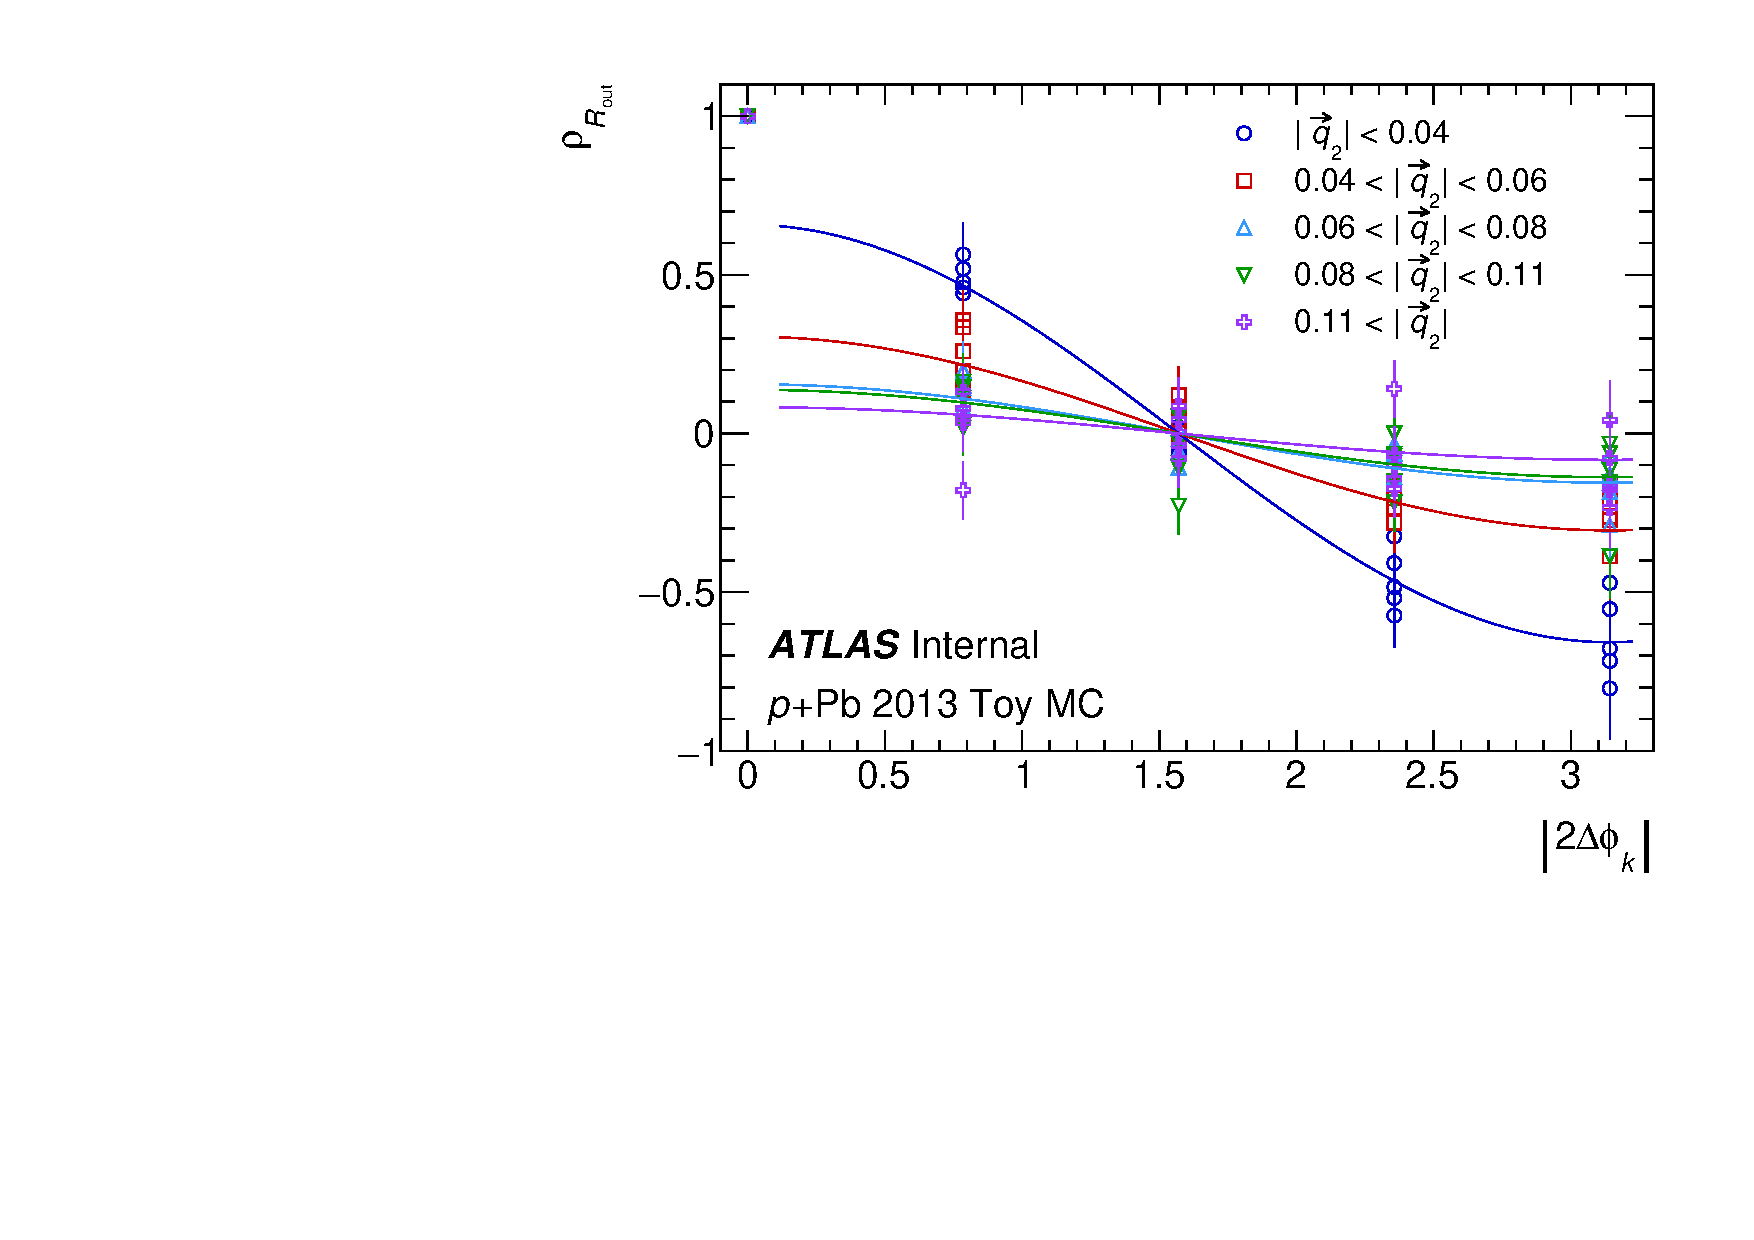
\includegraphics[width=.49\linewidth]{can_rho_Rout_dphi.pdf}
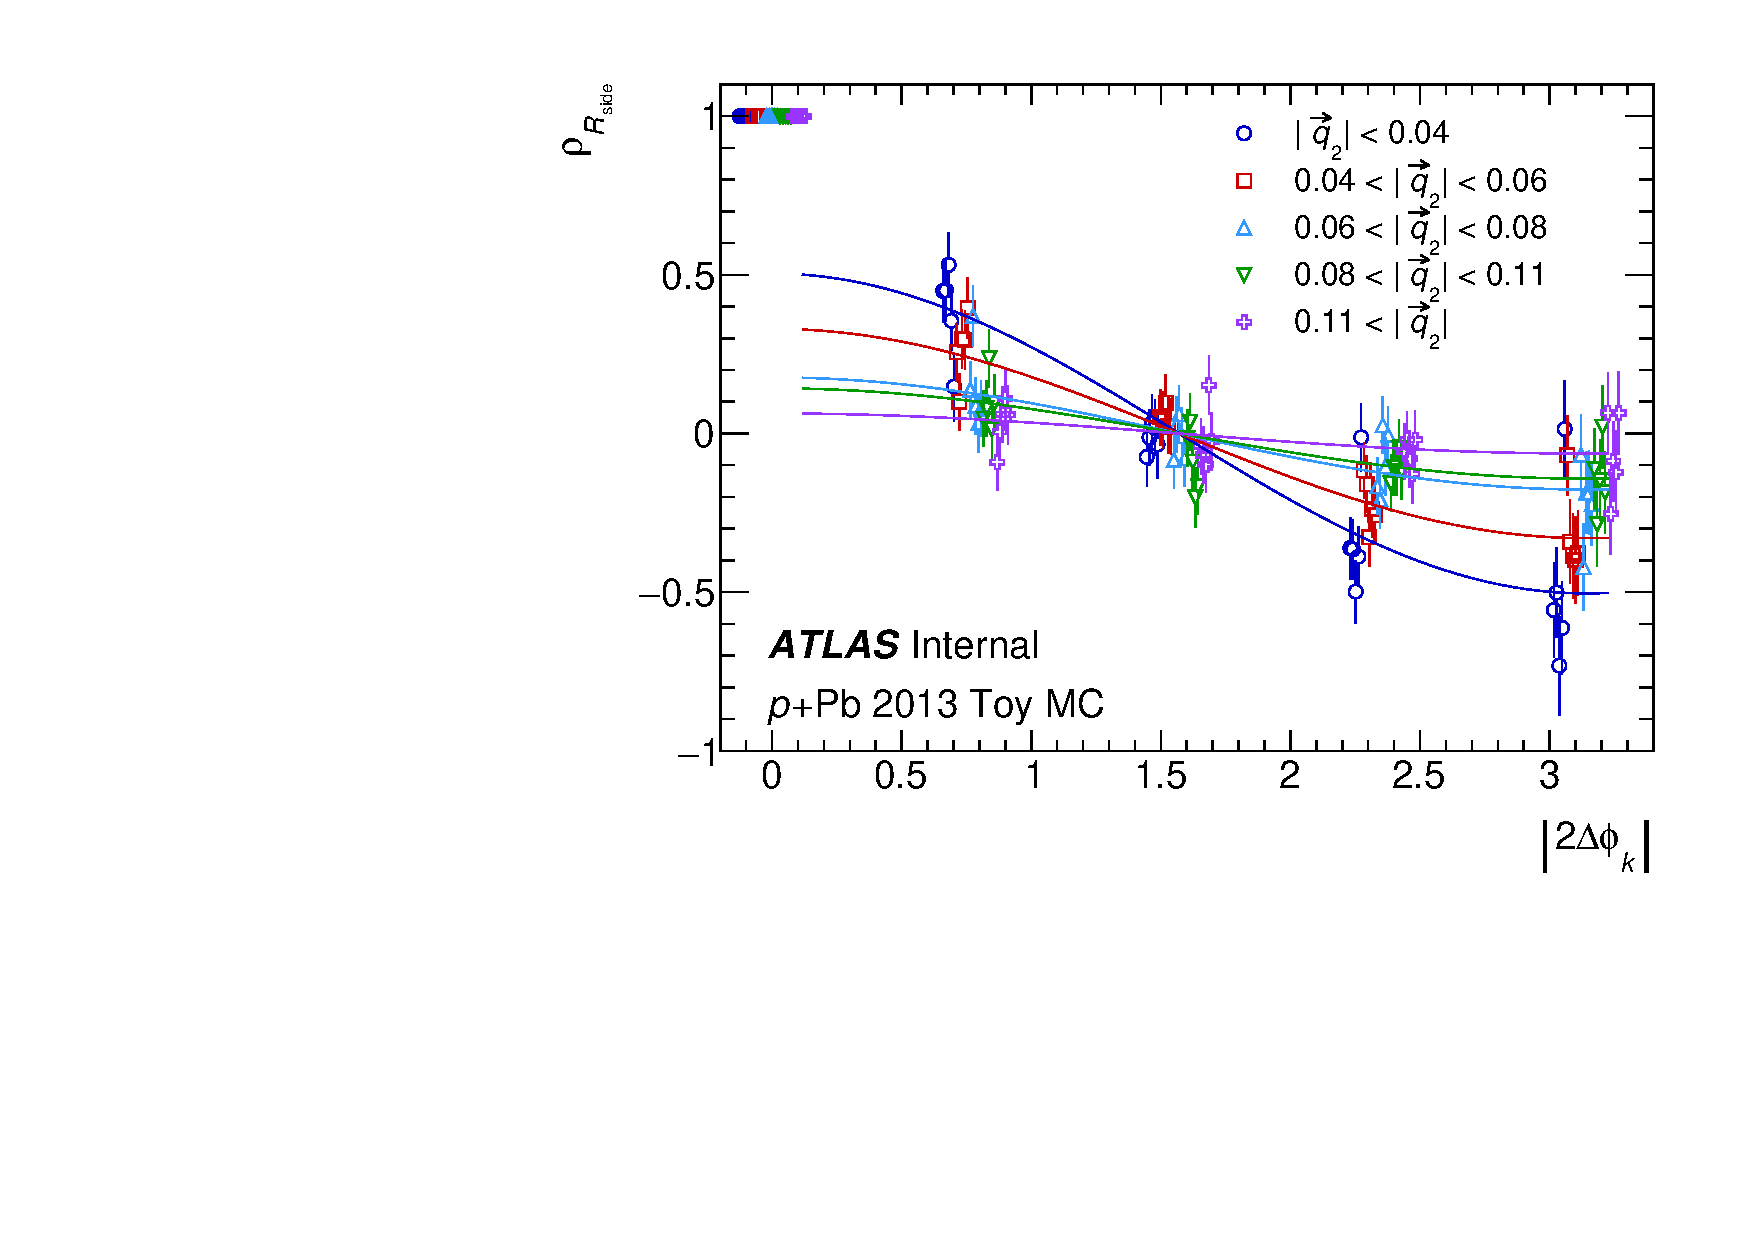
\includegraphics[width=.49\linewidth]{can_rho_Rside_dphi.pdf}
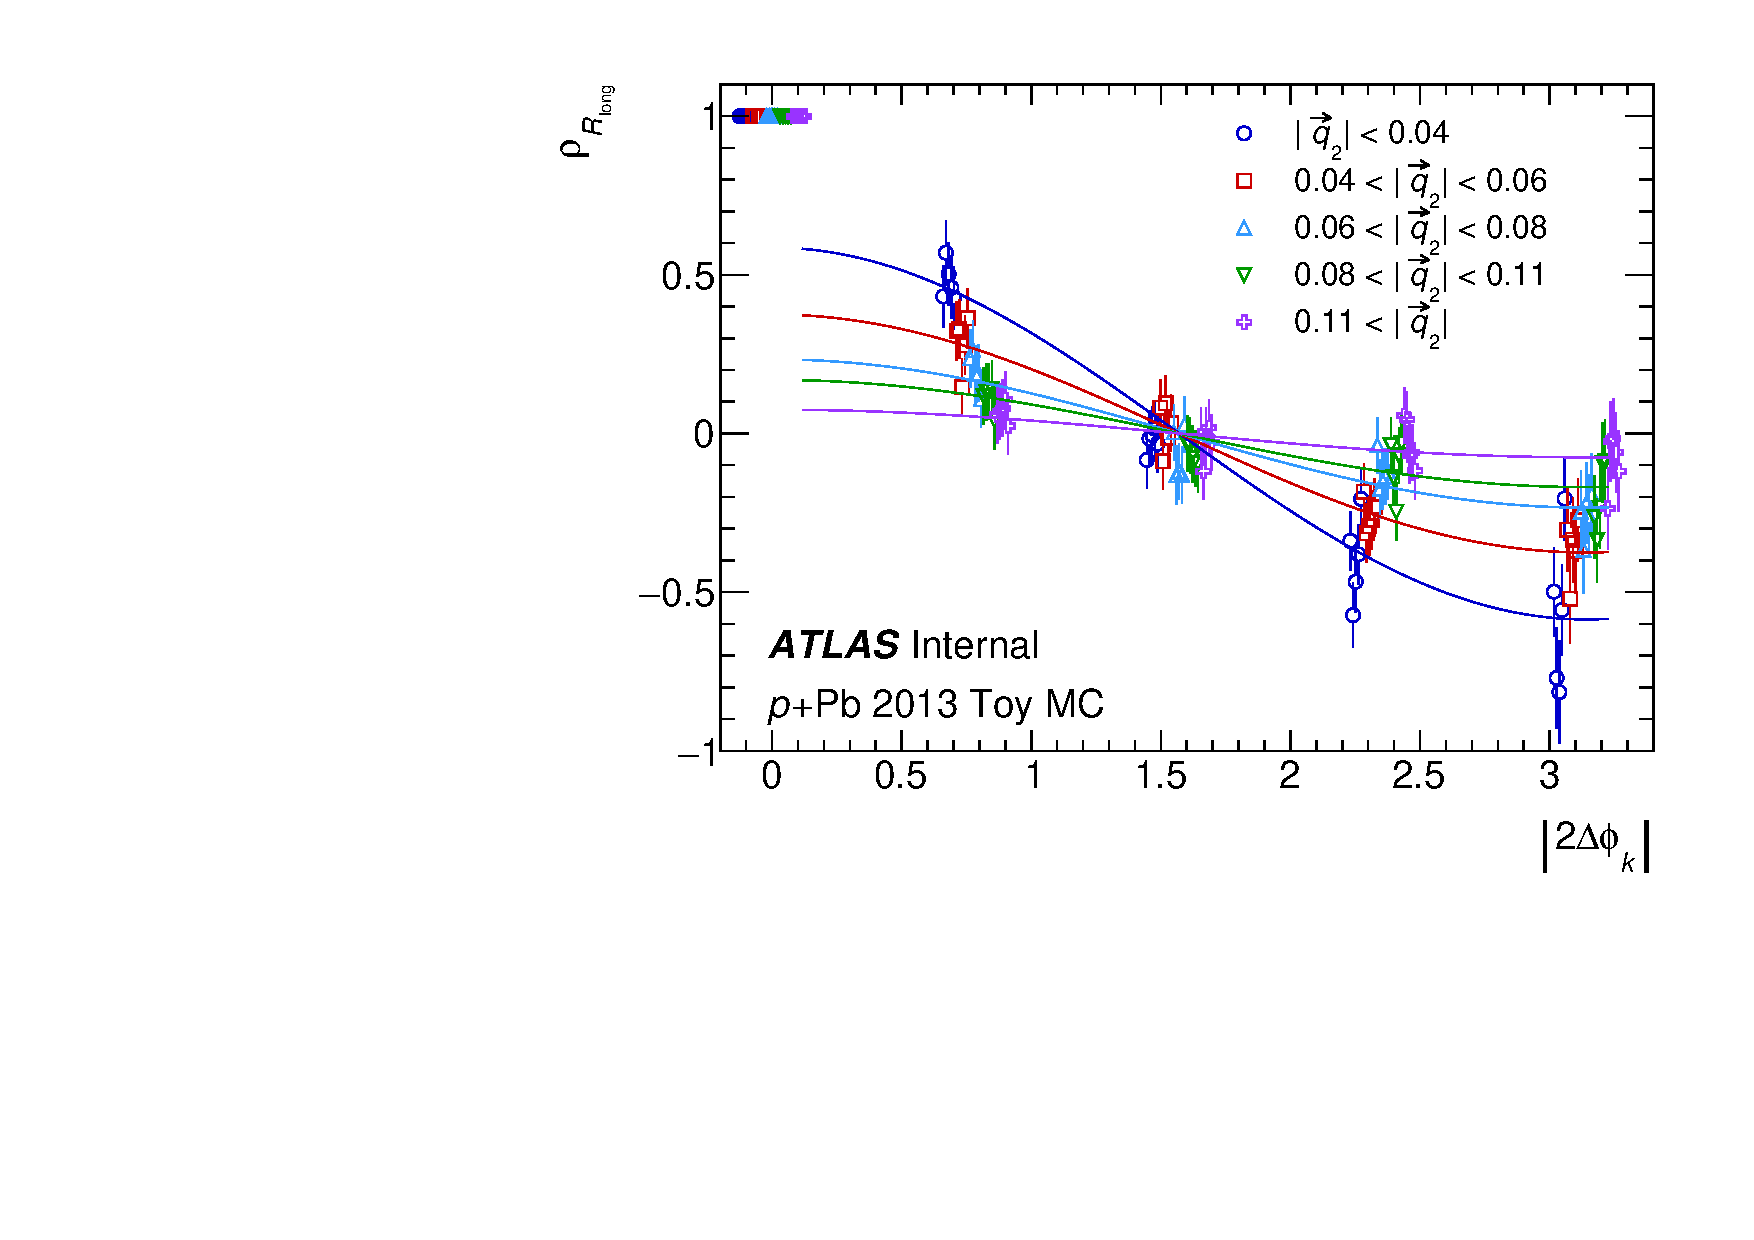
\includegraphics[width=.49\linewidth]{can_rho_Rlong_dphi.pdf}
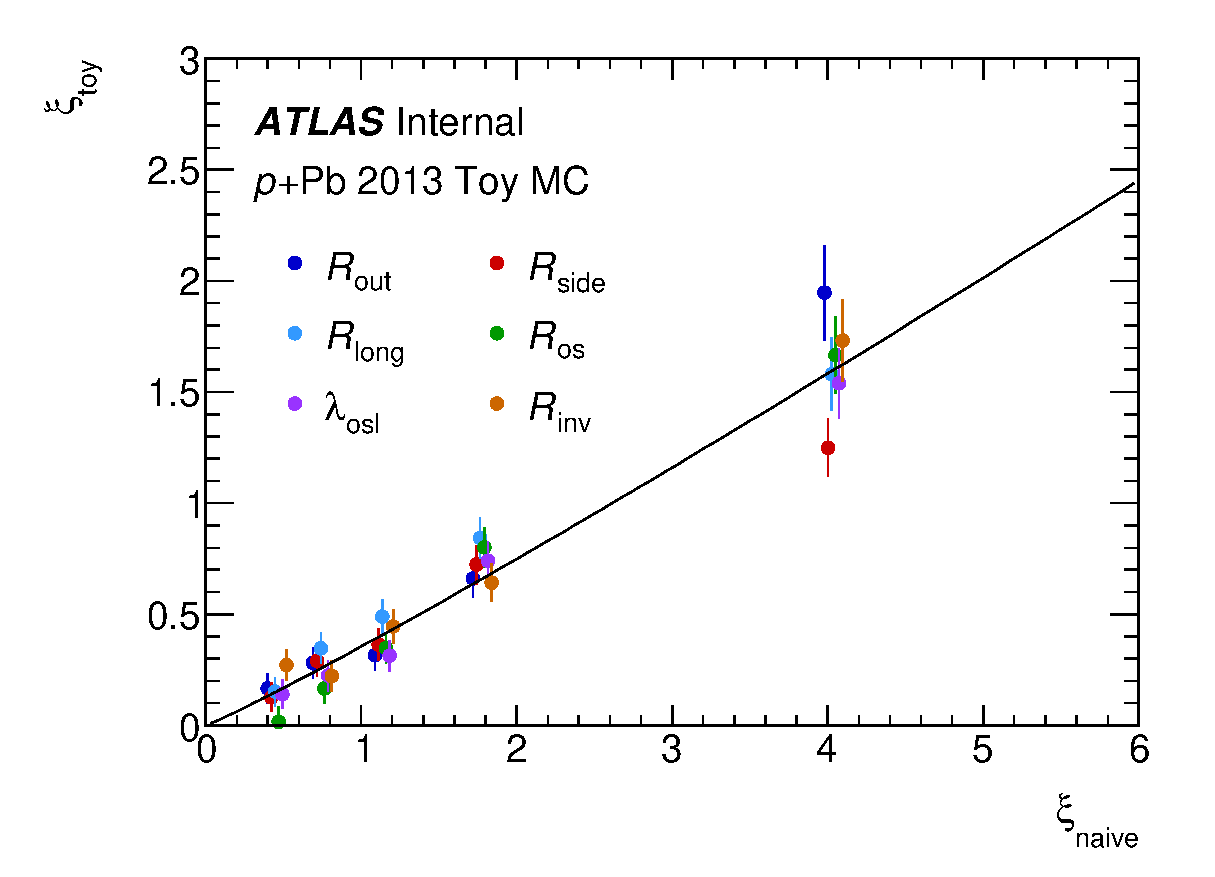
\includegraphics[width=.49\linewidth]{xi_comparison.eps}
\caption{The statistical correlation matrix elements for the HBT radii \Rout (top left), \Rside (top right), and \Rlong (bottom left) from a toy Monte Carlo study. In each $|\qt|$ interval the correlations are fit to a function $\rho = \frac{\Xi}{1+\Xi} \cos\left(2\Delta\kphi\right)$ for $2\Delta\kphi > 0$ where $\Xi \equiv \frac{2\xi(2+\xi)}{\Nbins}$ with $\Nbins = 8$. The correlation strength parameter $\xi$ from the toy study is shown as a function of the naive value of $\xi$ (bottom right), which determines the azimuthal statistical correlations in the HBT radii.}
\label{fig:rho_dphi}
\end{figure}

These correlations have a large impact on the uncertainties of these components at low flow $|\qt|$, where the event plane resolution correction is the largest.



\FloatBarrier
\section{Hard-process correlations}
\label{sec:jet_frag}

An additional contribution to the correlation function with a width in \qinv of order 0.5--1 \GeV\ arises from hard processes in the event.
It is more prominent at high \kt, which suggests that the correlation comes from jet fragmentation.
This origin of the effect was confirmed by running \Hijing with the minimum \pt for hard scattering turned up to $20 \GeV$ from the default of $2 \GeV$, which causes this feature to diminish as shown in \cref{fig:hard_process_min_pt}.
\Hijing has no Coulomb or Bose-Einstein effects, so any effects in \cref{fig:hard_process_min_pt} are from charge/momentum conservation, resonance decays, and jet fragmentation.
The effect is more pronounced at high \kt and low multiplicities, where particle pairs are more likely to have come from the same mini-jet.

It should be noted that \ac{MC} generators all tend to over-estimate the amplitude of the contribution from hard processes.
In the past a double ratio, i.e. the ratio of the correlation function in data to \ac{MC}, has been used but this produces a suspicious depletion in the affected \qinv region.


\begin{figure}[t]
% 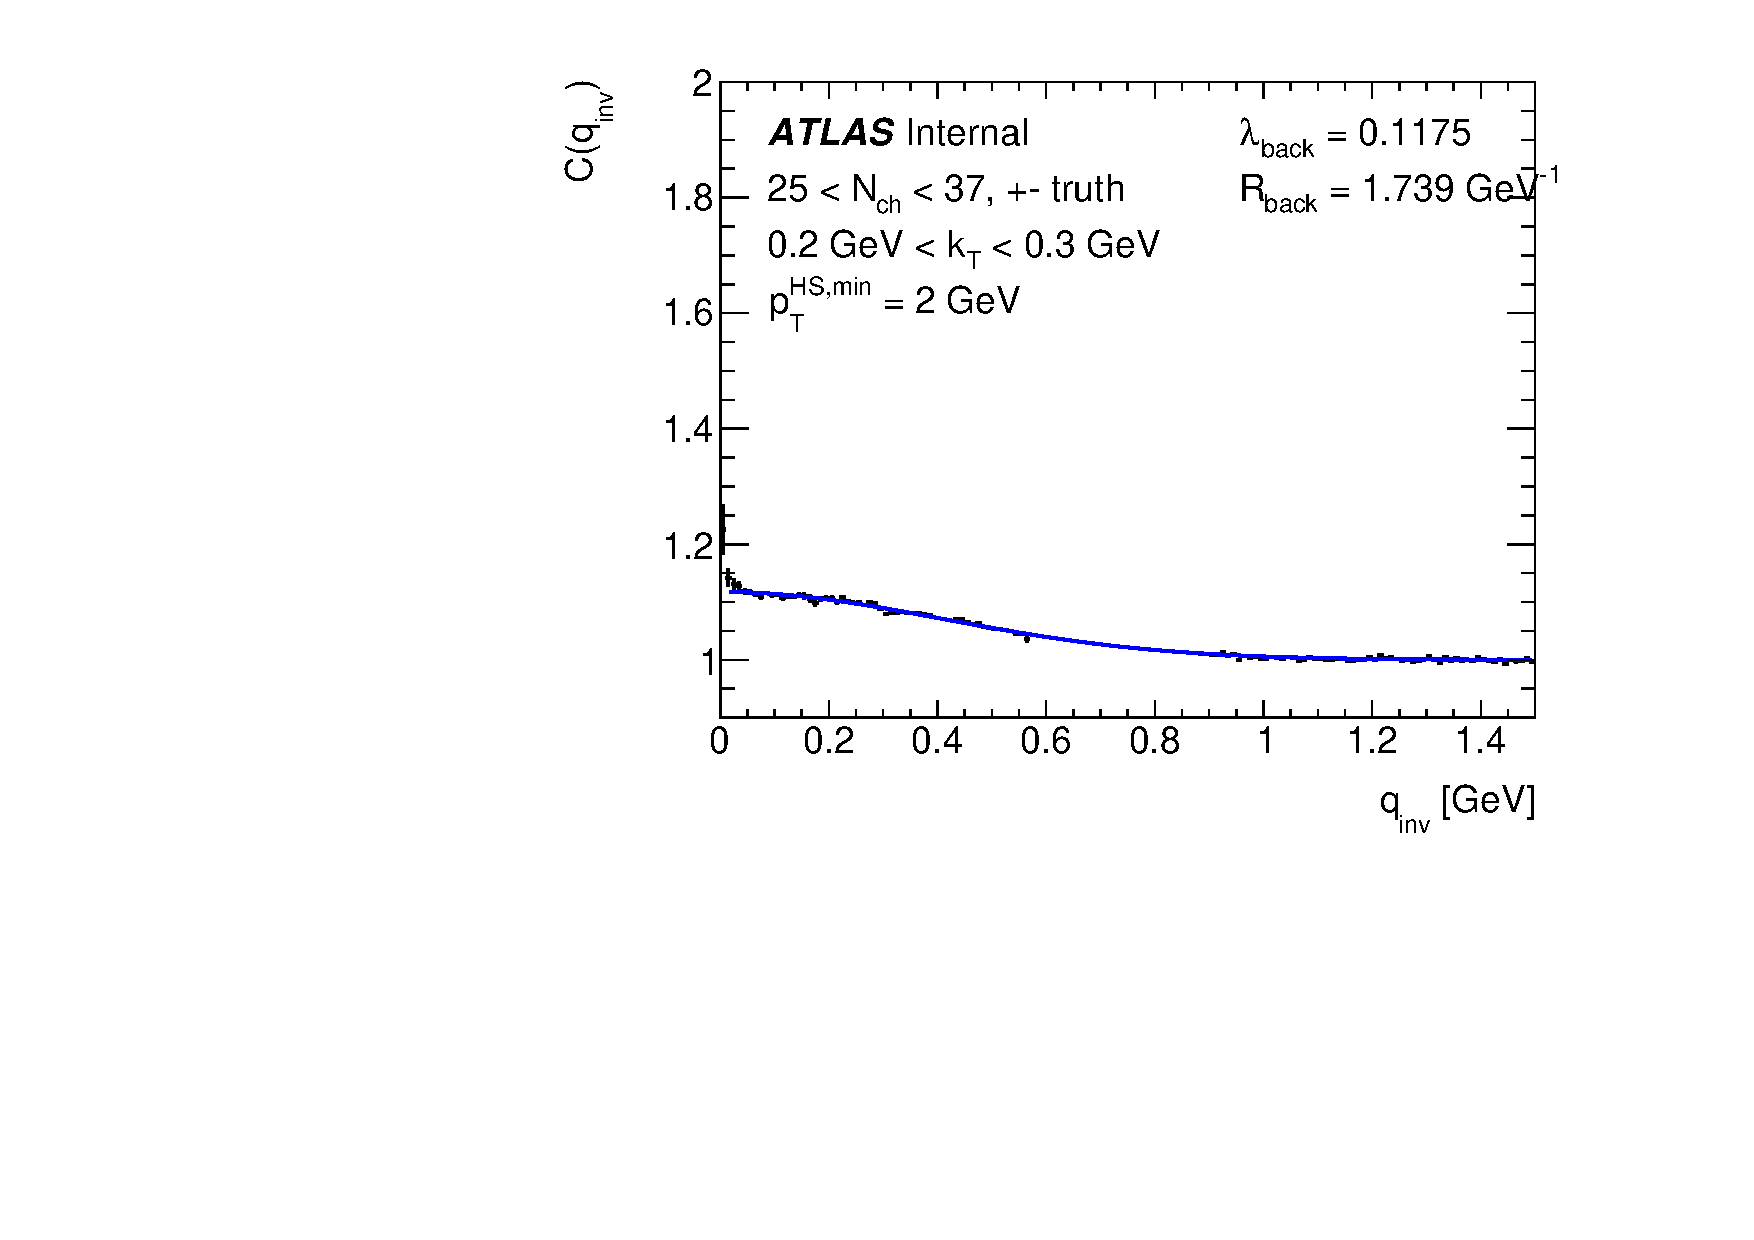
\includegraphics[width=.4\linewidth]{Cqinv_Nch26to36_e0_kt1_pPbHijing.pdf}
% 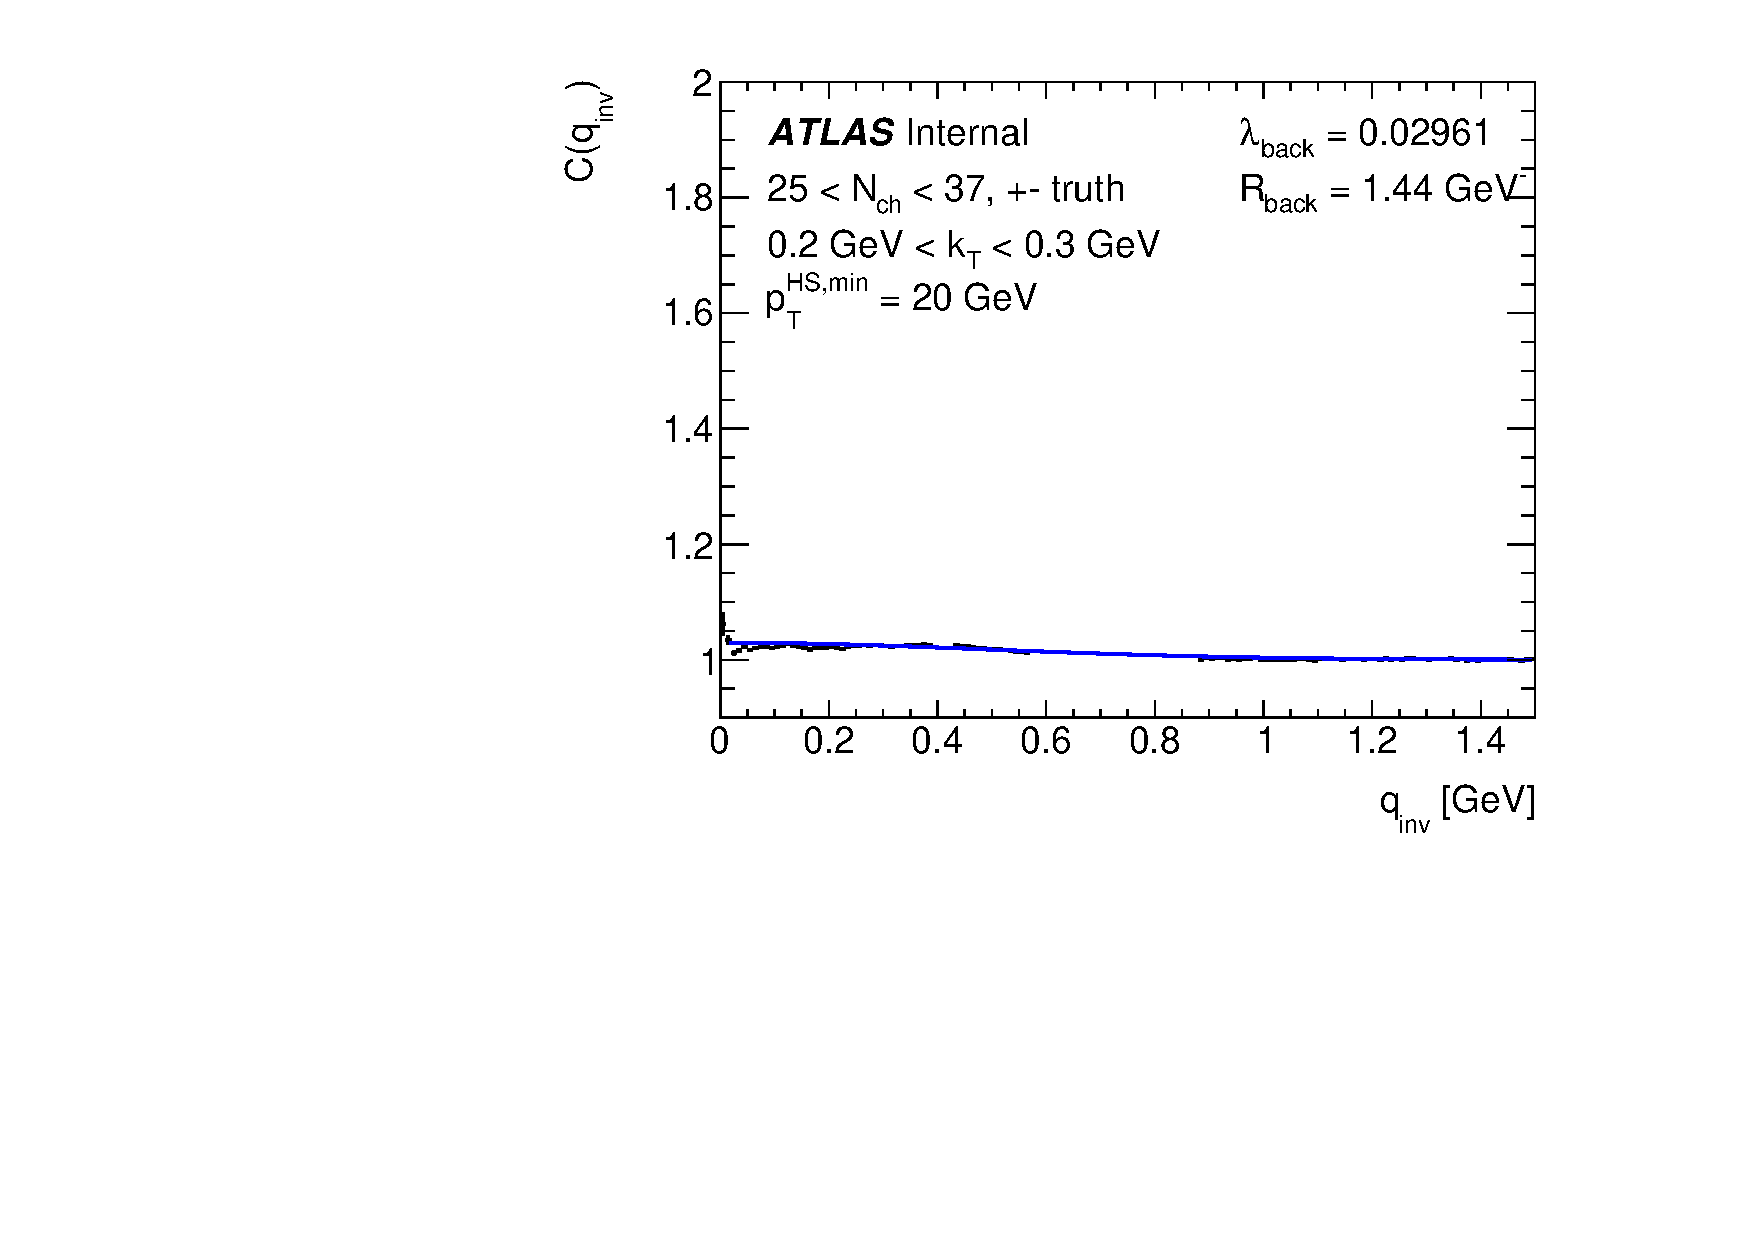
\includegraphics[width=.4\linewidth]{Cqinv_Nch26to36_e0_kt1_pPbHijing20.pdf}
% 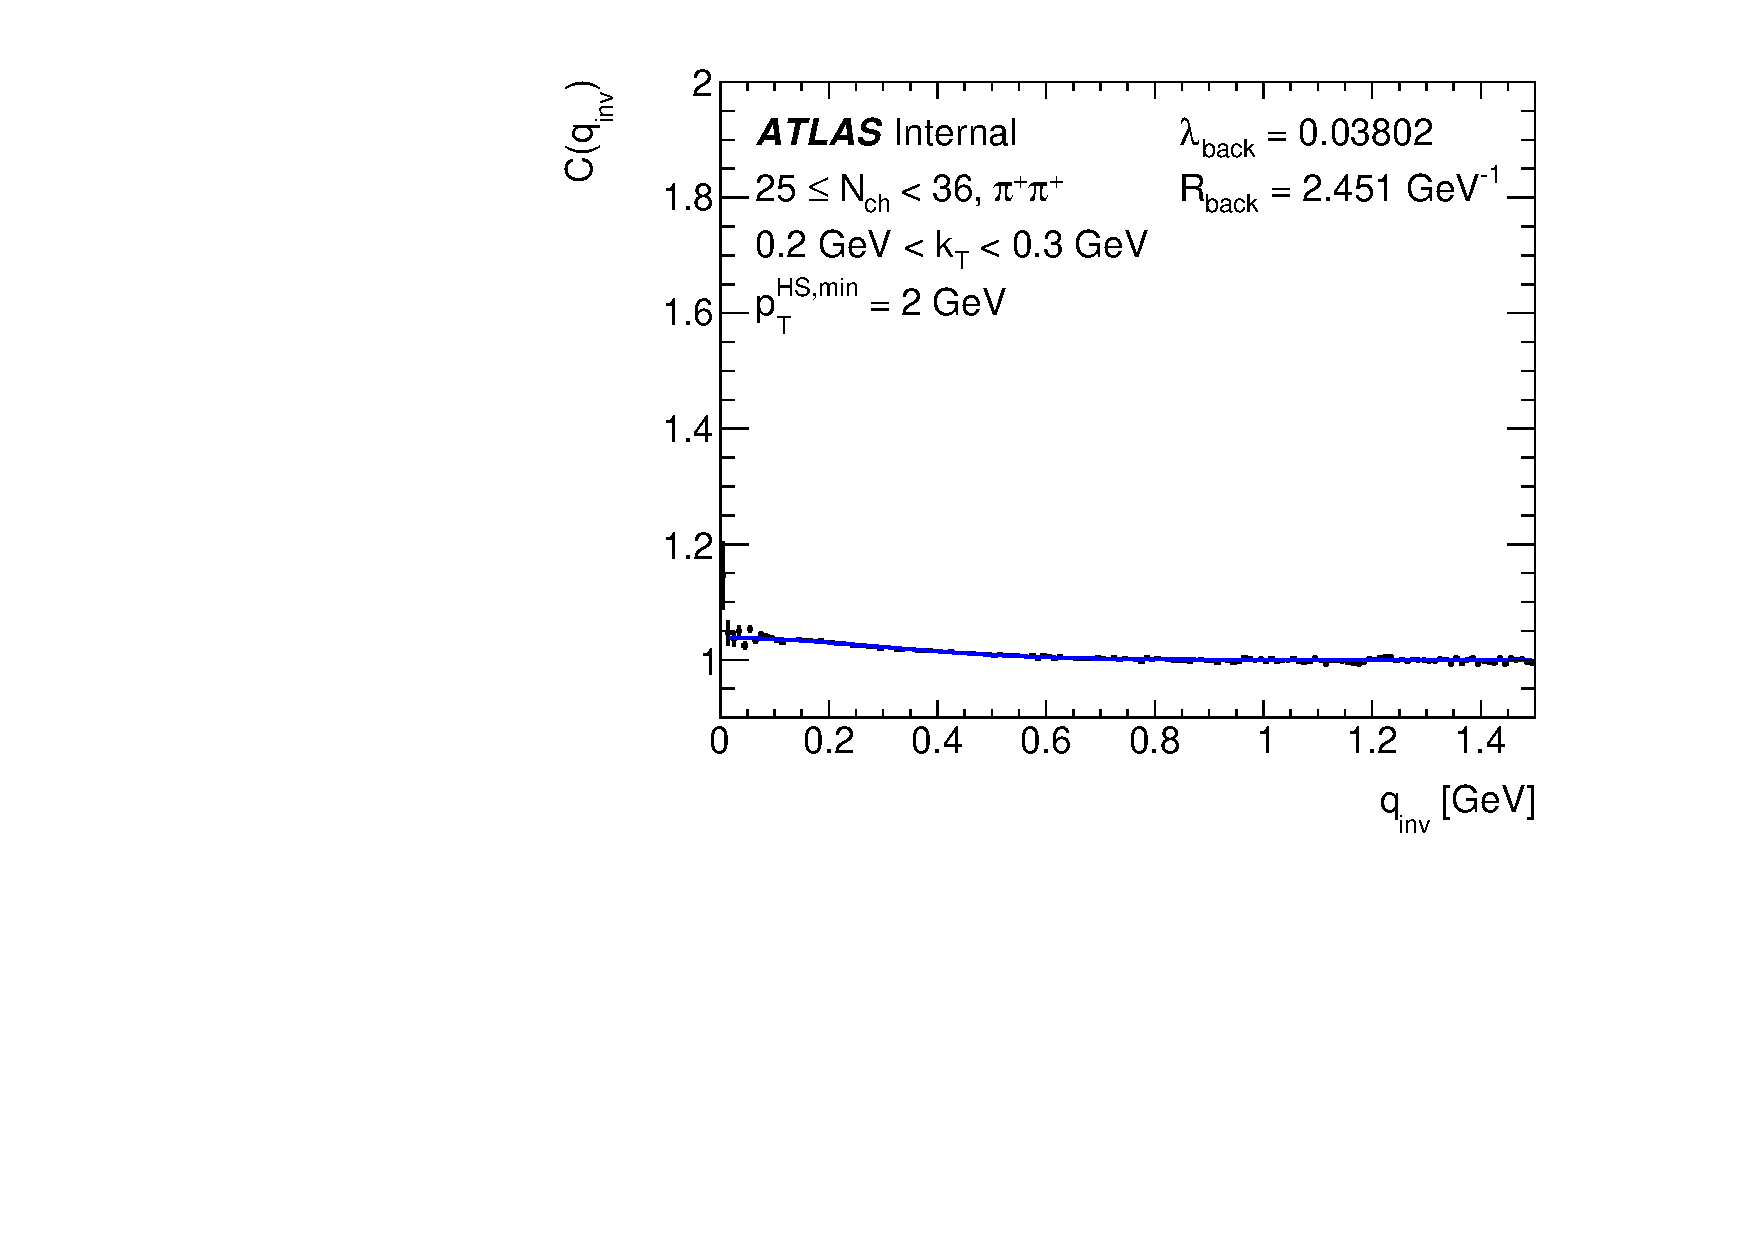
\includegraphics[width=.4\linewidth]{Cqinv_Nch26to36_e1_kt1_pPbHijing.pdf}
% 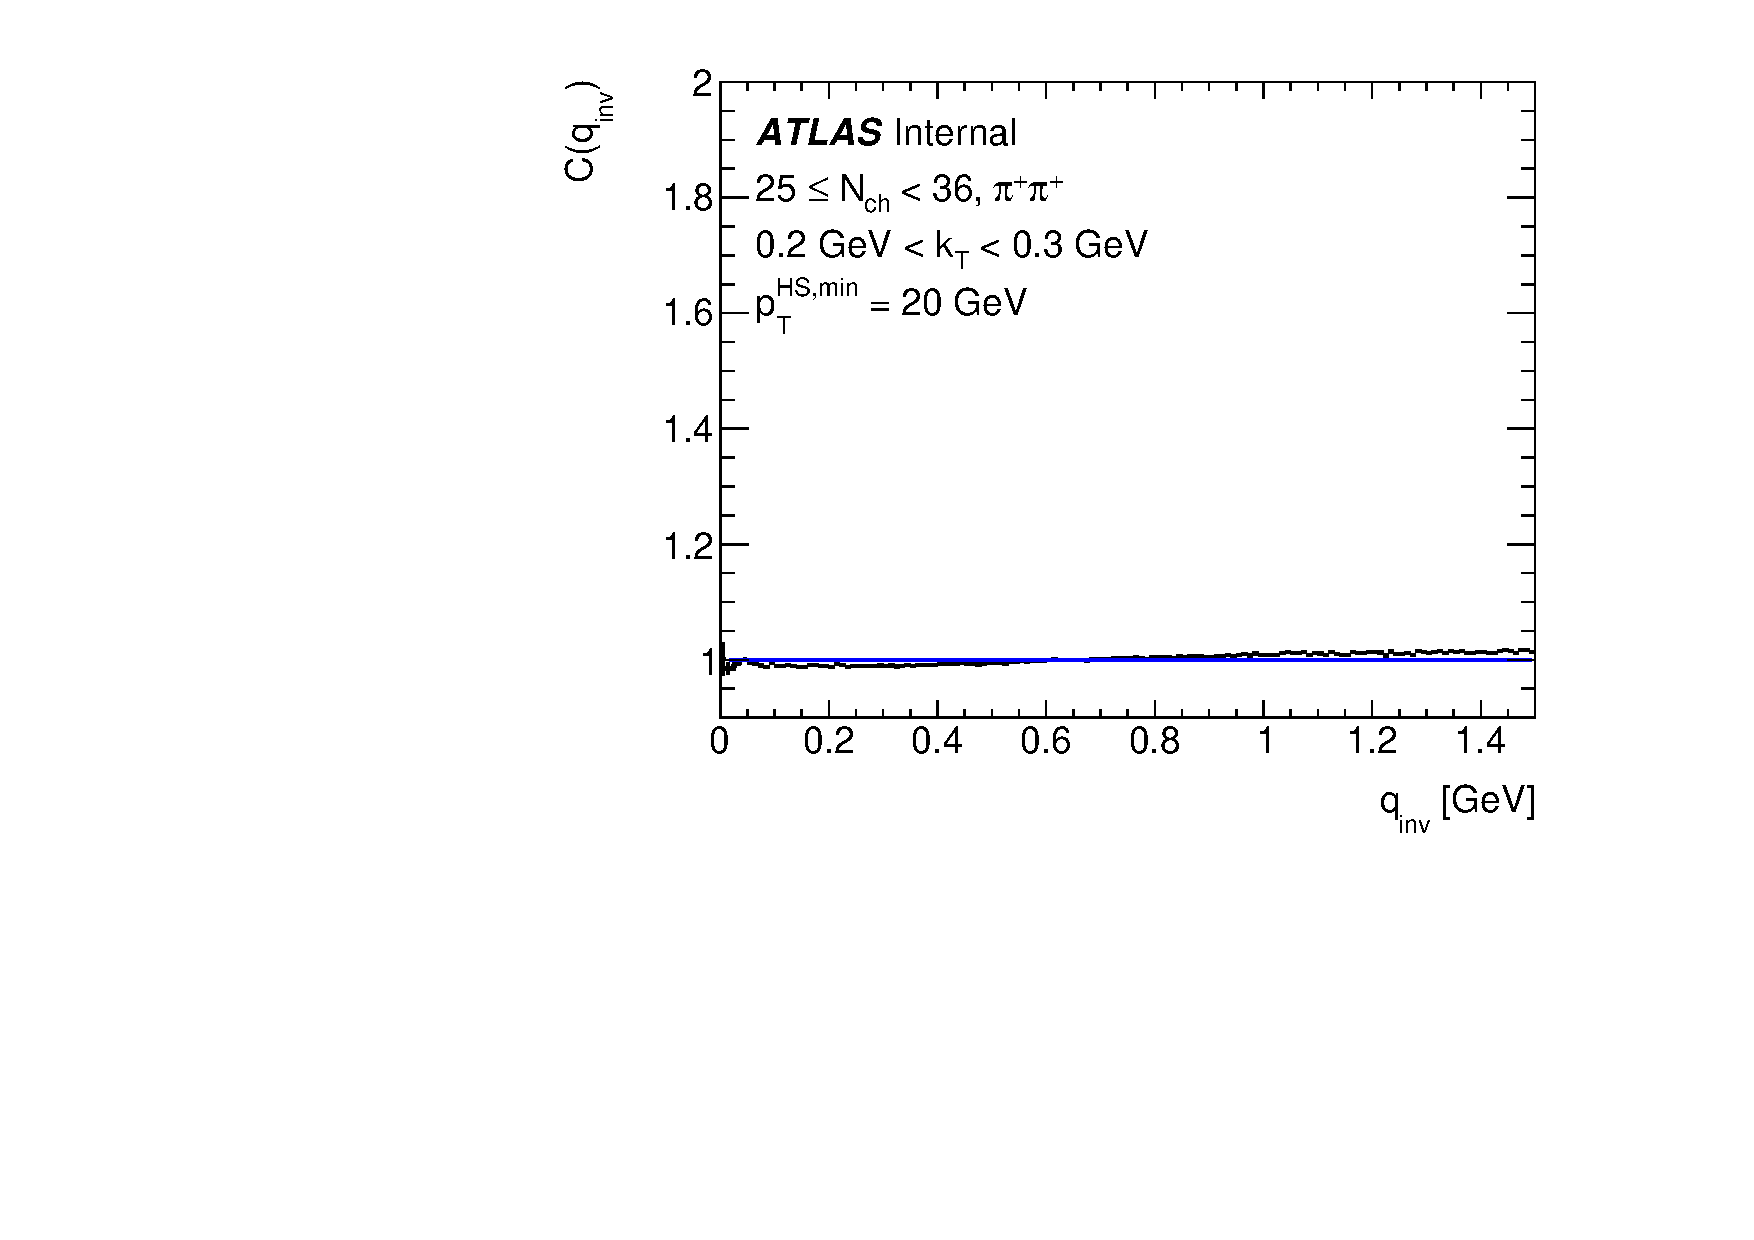
\includegraphics[width=.4\linewidth]{Cqinv_Nch26to36_e1_kt1_pPbHijing20.pdf}
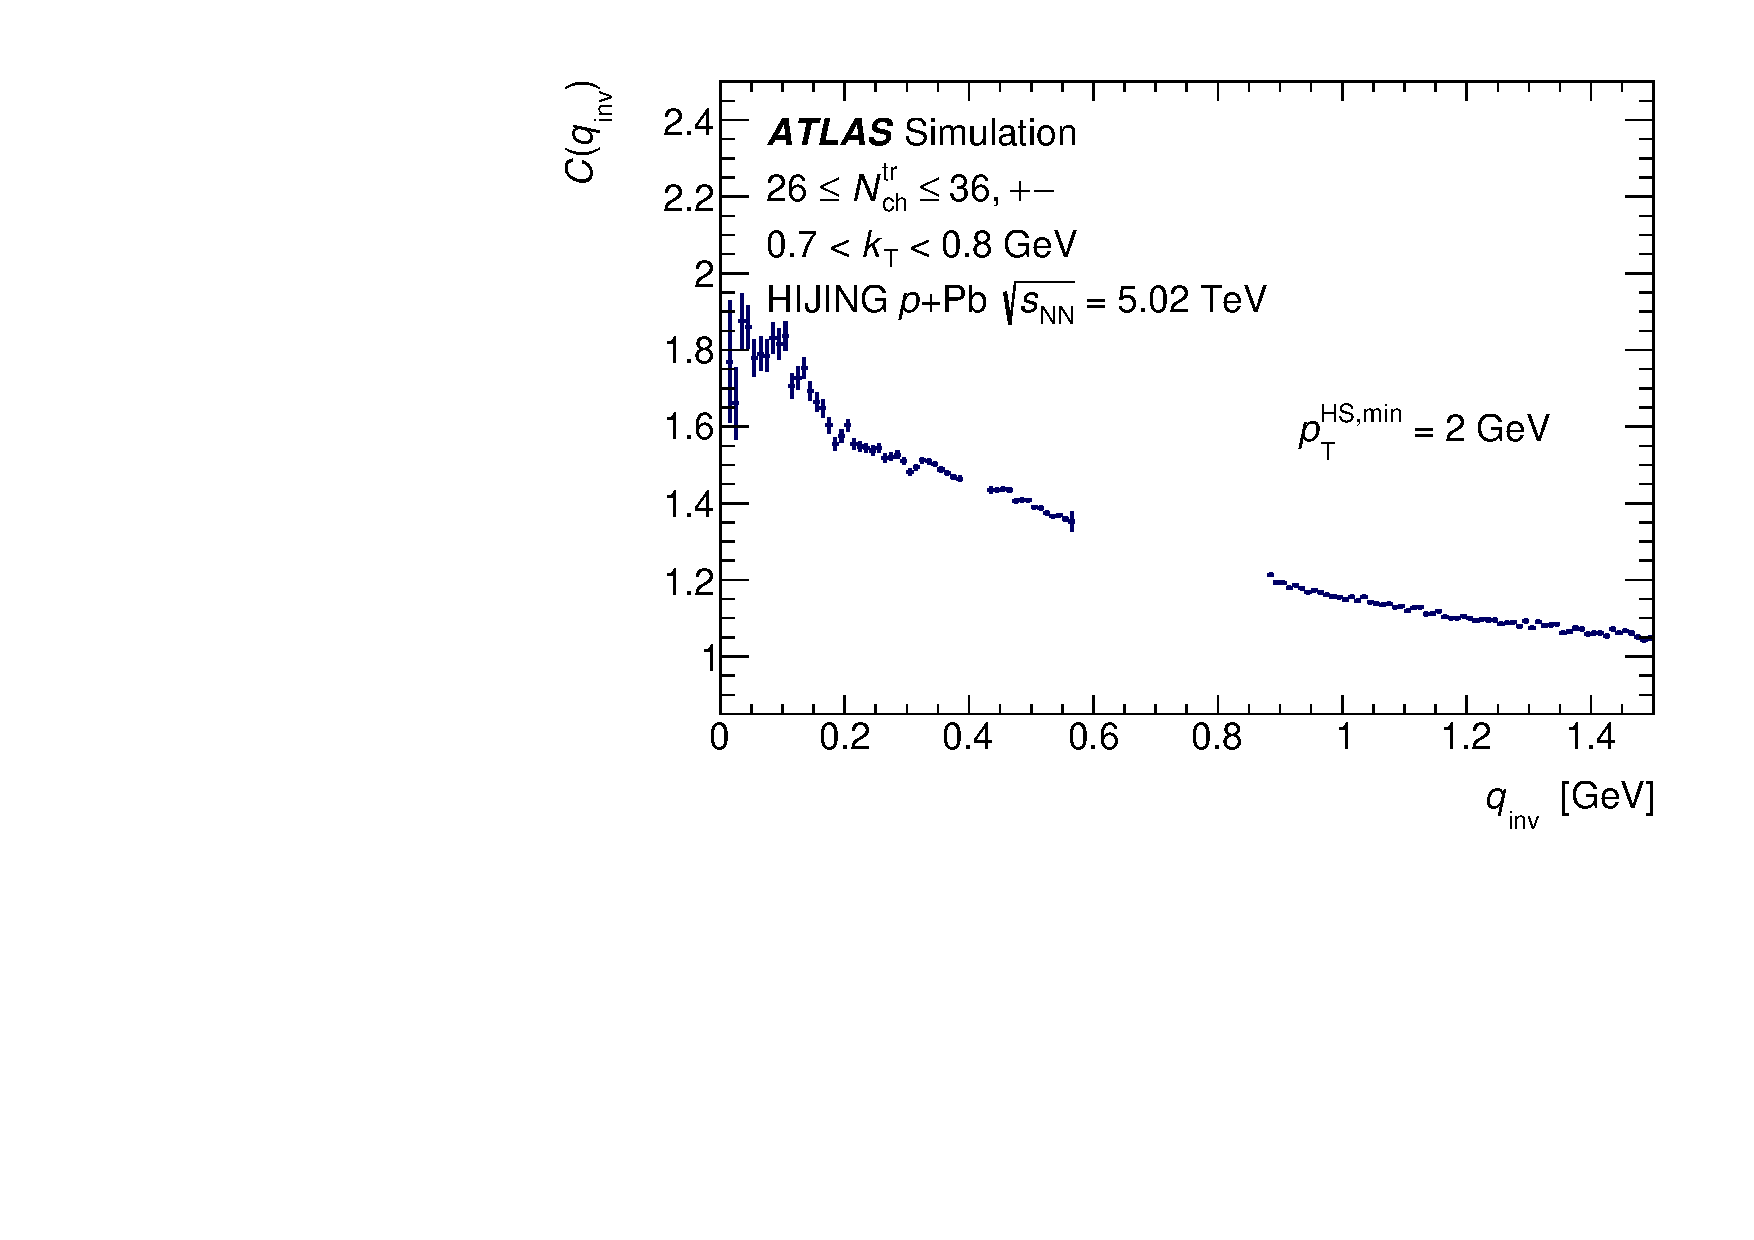
\includegraphics[width=.49\linewidth]{Cqinv_Nch26to36_e0_kt6_pPbHijing.pdf}
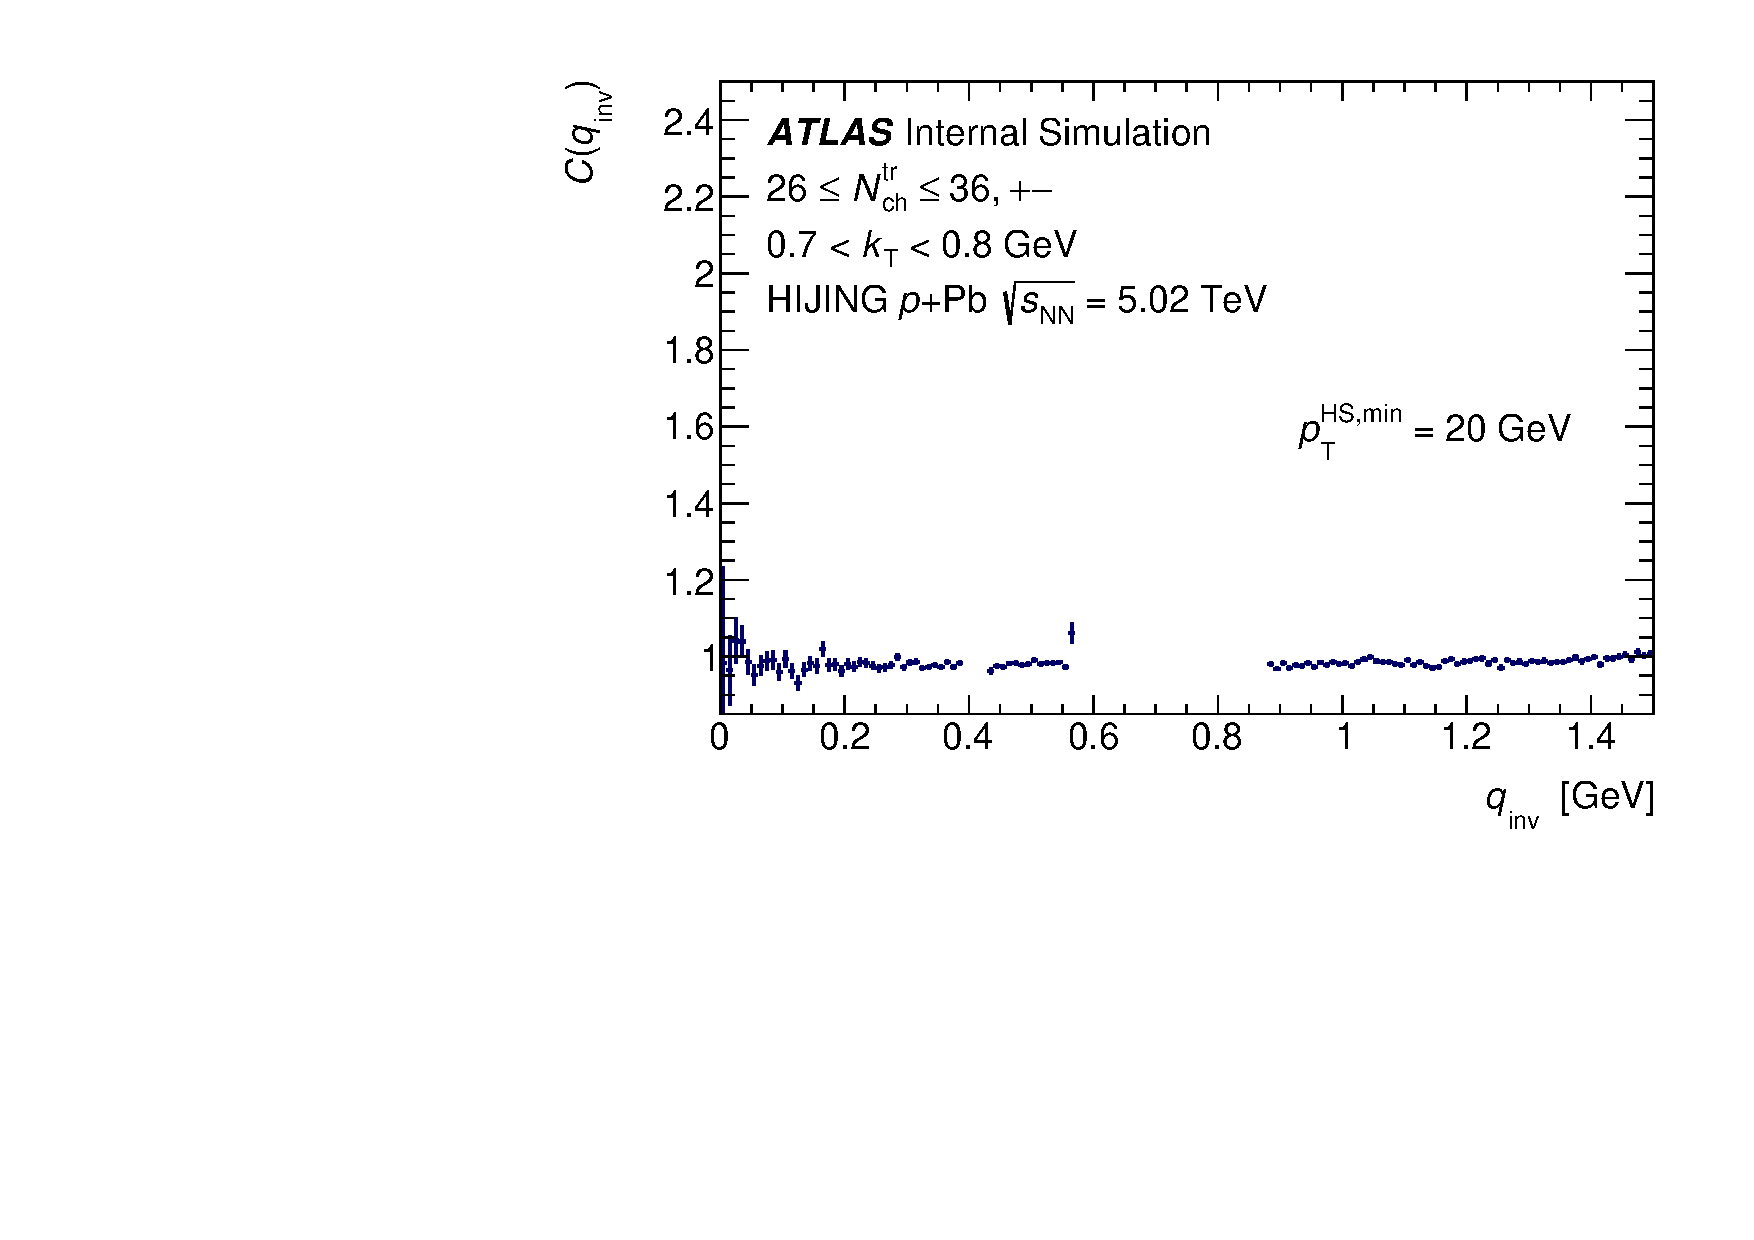
\includegraphics[width=.49\linewidth]{Cqinv_Nch26to36_e0_kt6_pPbHijing20.pdf}
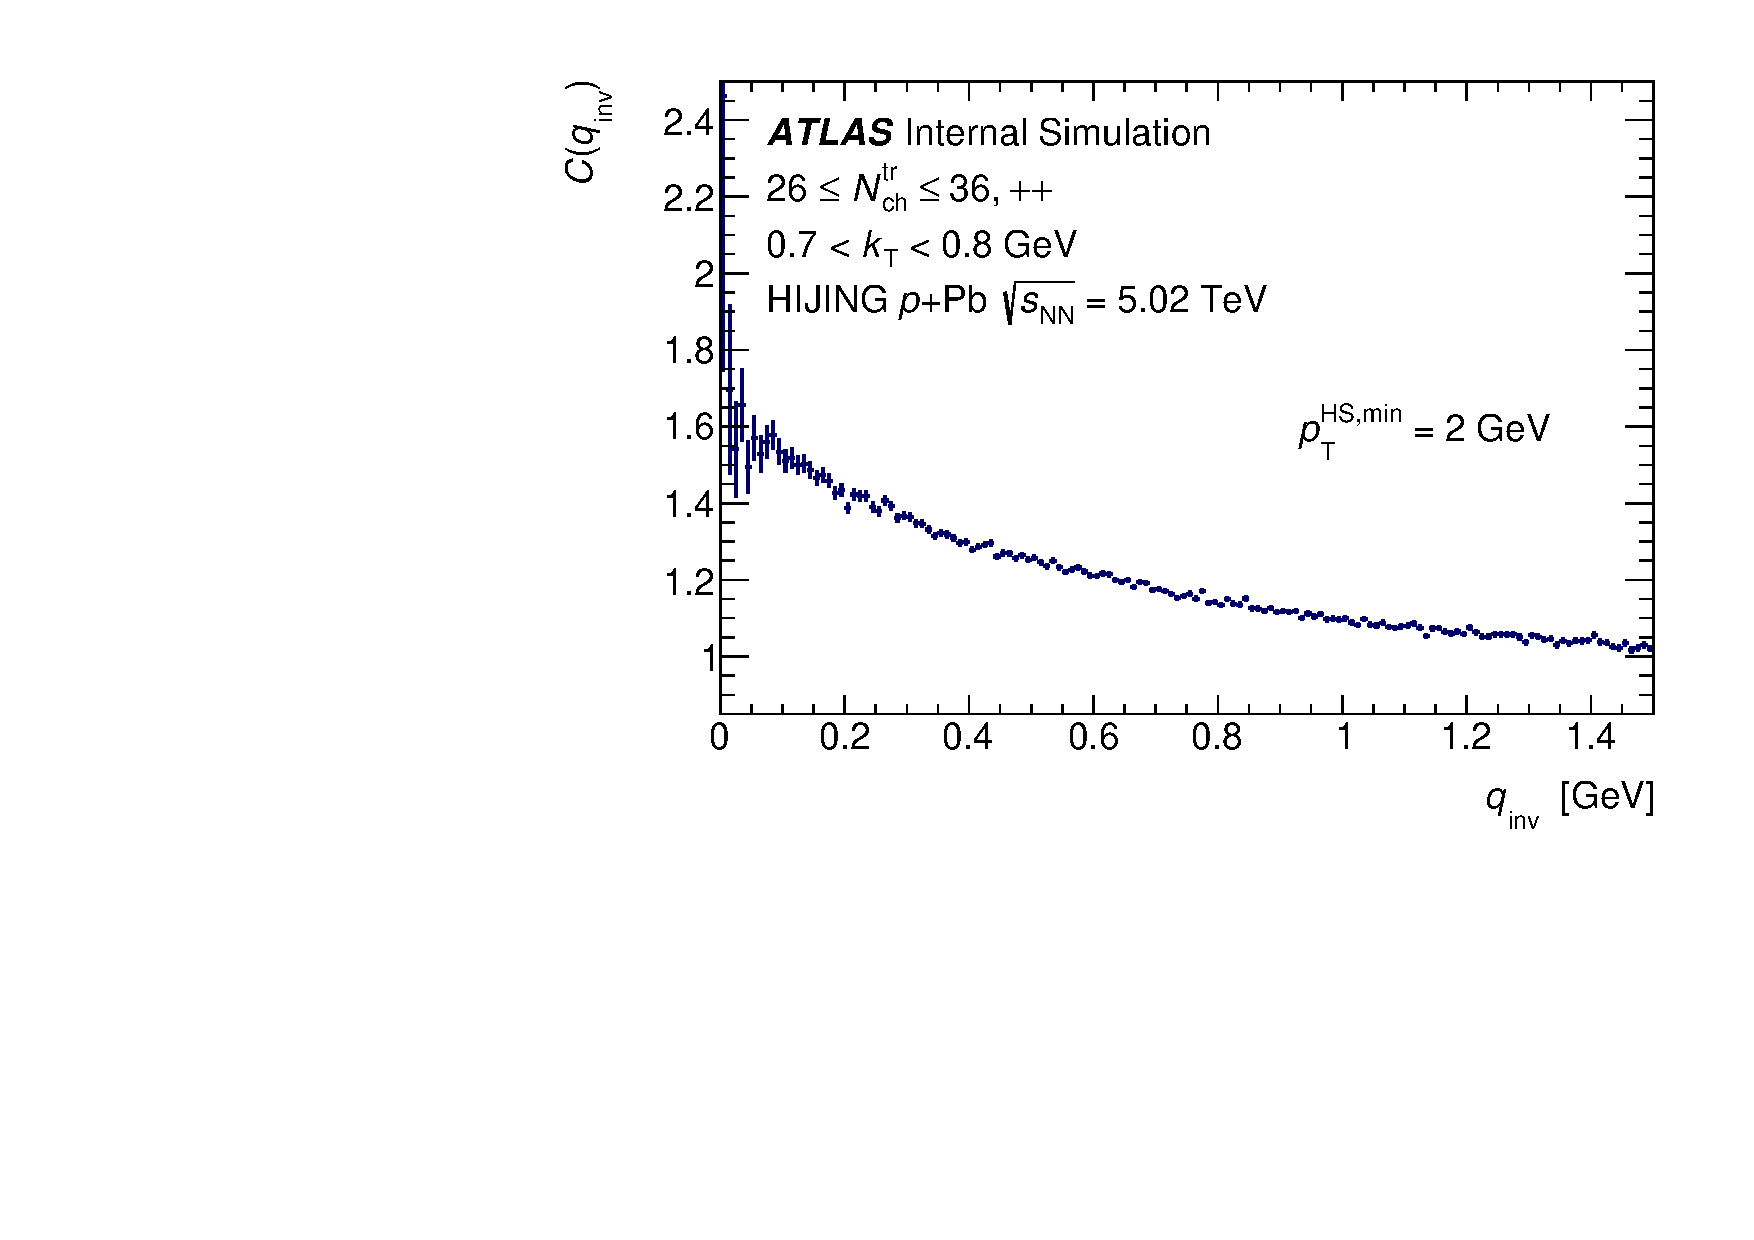
\includegraphics[width=.49\linewidth]{Cqinv_Nch26to36_e1_kt6_pPbHijing.pdf}
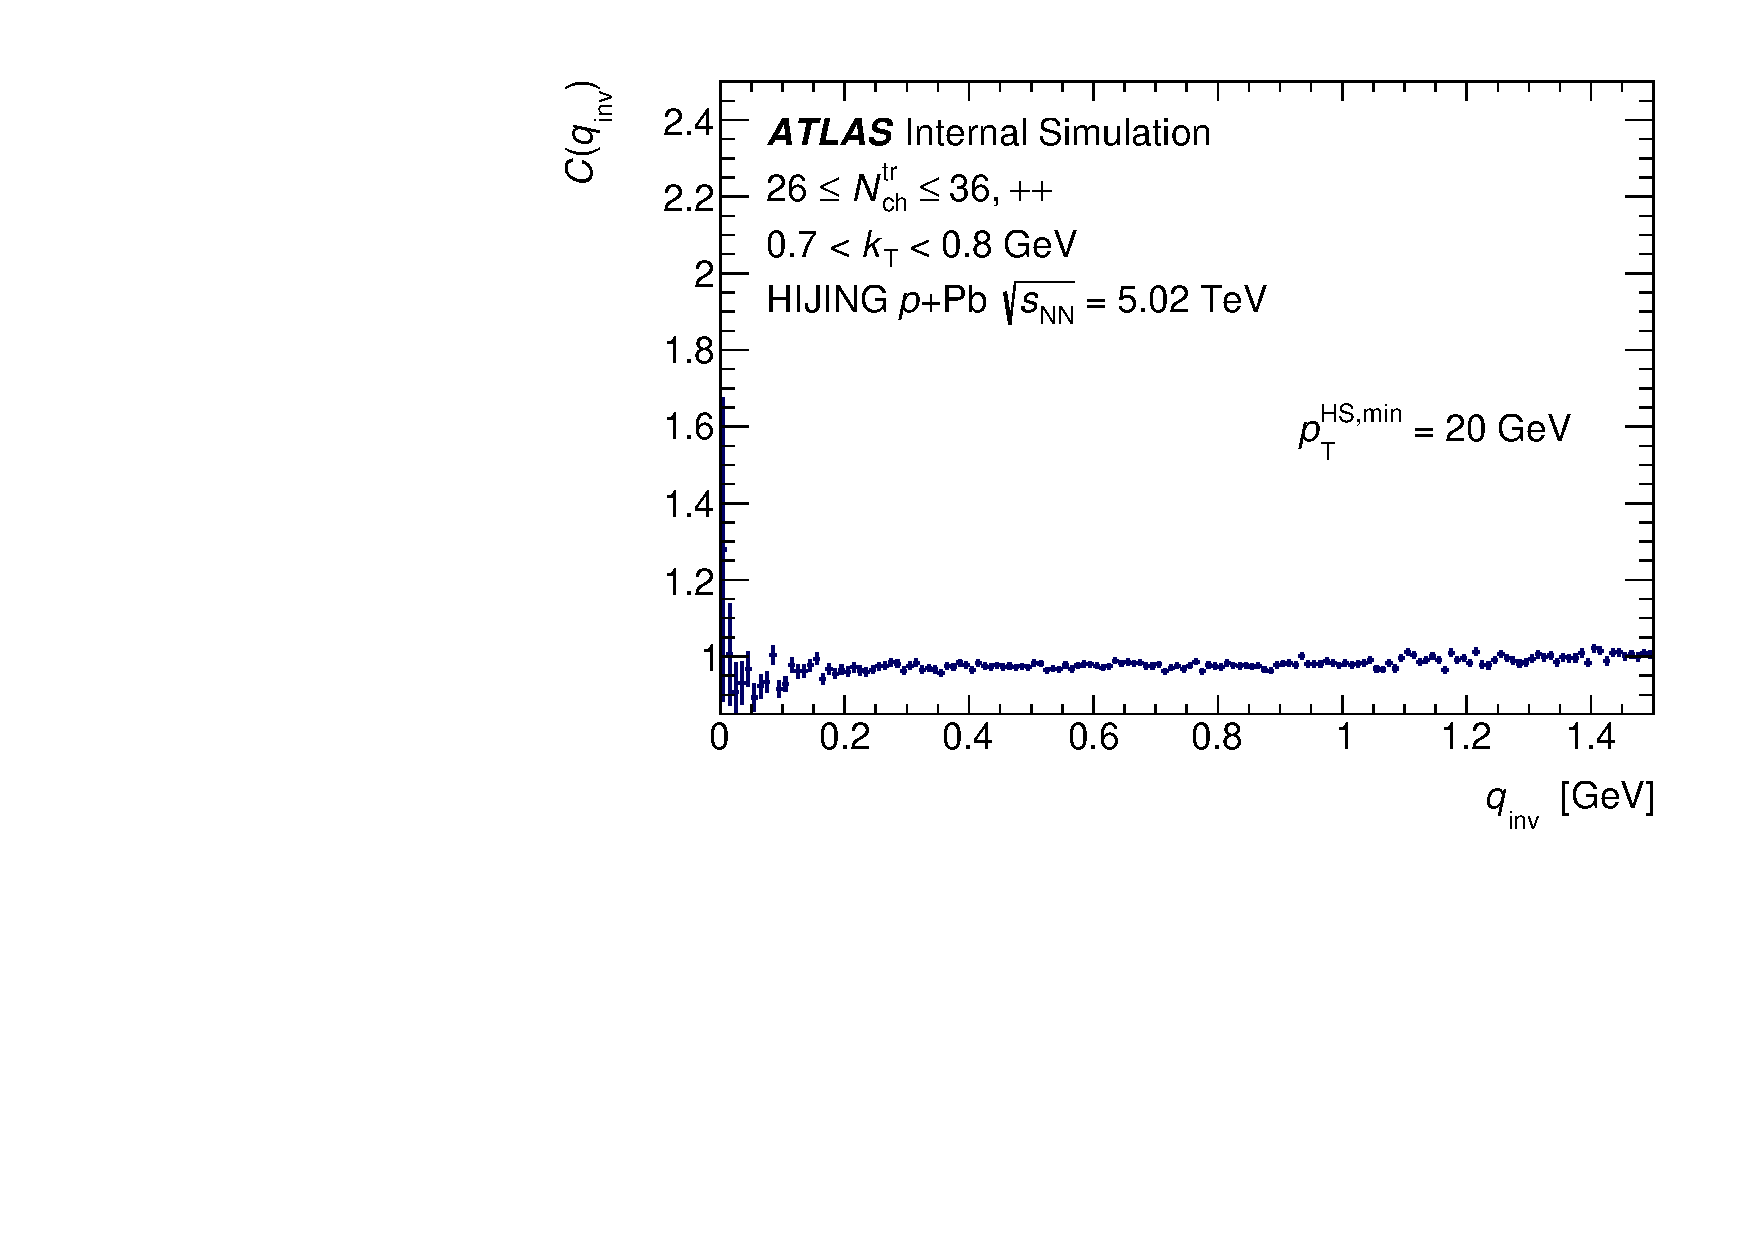
\includegraphics[width=.49\linewidth]{Cqinv_Nch26to36_e1_kt6_pPbHijing20.pdf}
\caption{The hard-process background in \Hijing for either $+-$ or $++$ charged pairs with major resonances removed from $+-$, with the minimum hard-scattering \pt set to the default of $2 \GeV$ (left) and turned up to $20 \GeV$ (right). Removing the hard-scattering processes in this range diminishes or removes the non-femtoscopic signal. The Gaussian fits are shown only to roughly indicate the amplitude and width of the effects, and are not used in the analysis.}
\label{fig:hard_process_min_pt}
\end{figure}

\begin{figure}[t]
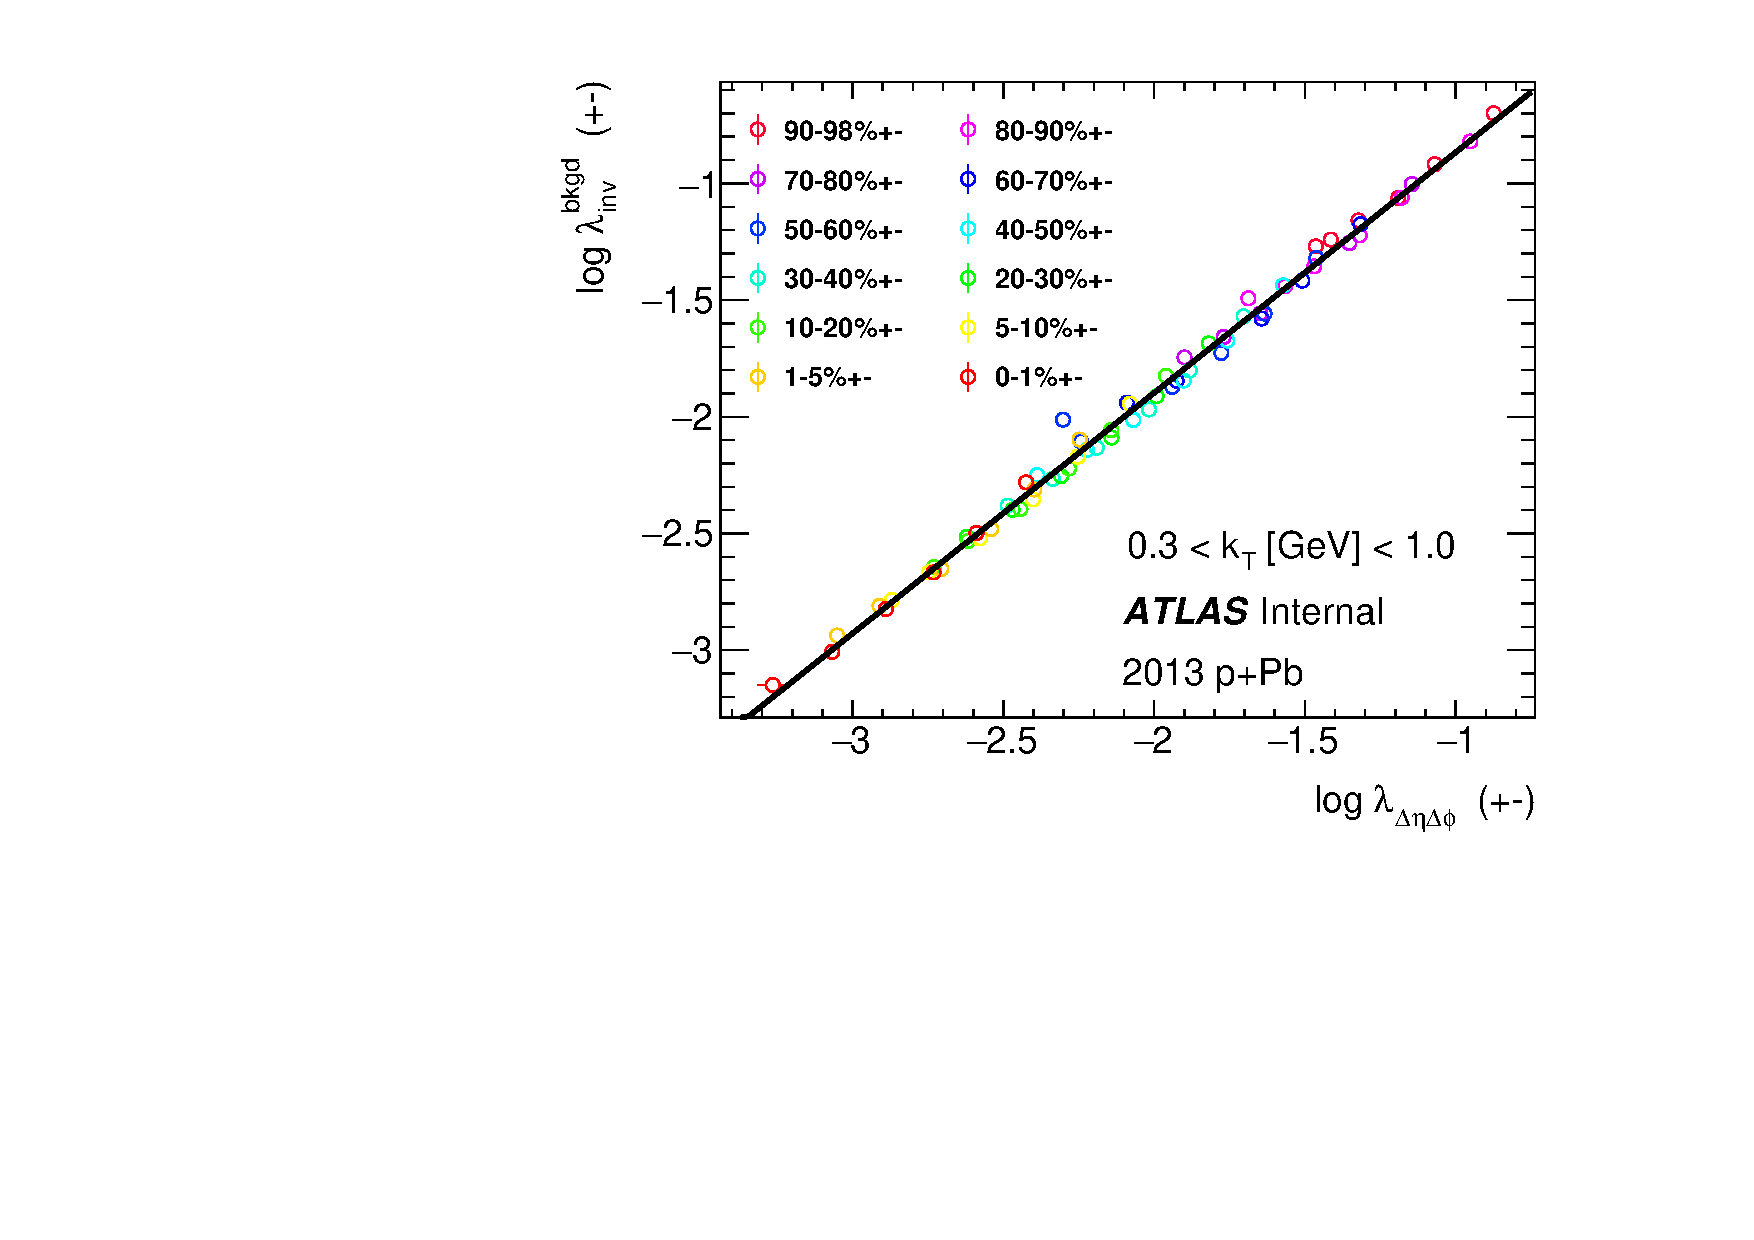
\includegraphics{qinv_backLambda_vs_ang_backLambda.pdf}
\caption{A comparison of the amplitudes of gaussian fits of the $\qinv$ and angular ($\Delta \eta, \Delta \phi$) correlation functions from opposite-sign pairs in the data. The pairs are fully Coulomb-corrected (i.e. $\lambda = 1$) with an effective source size of $\Reff = 1 \textrm{ fm}$. The different colors are different centralities, each with a range of \kt.}
\label{fig:background_amp_inv_vs_ang_data}
\end{figure}

\begin{figure}[t]
\centering
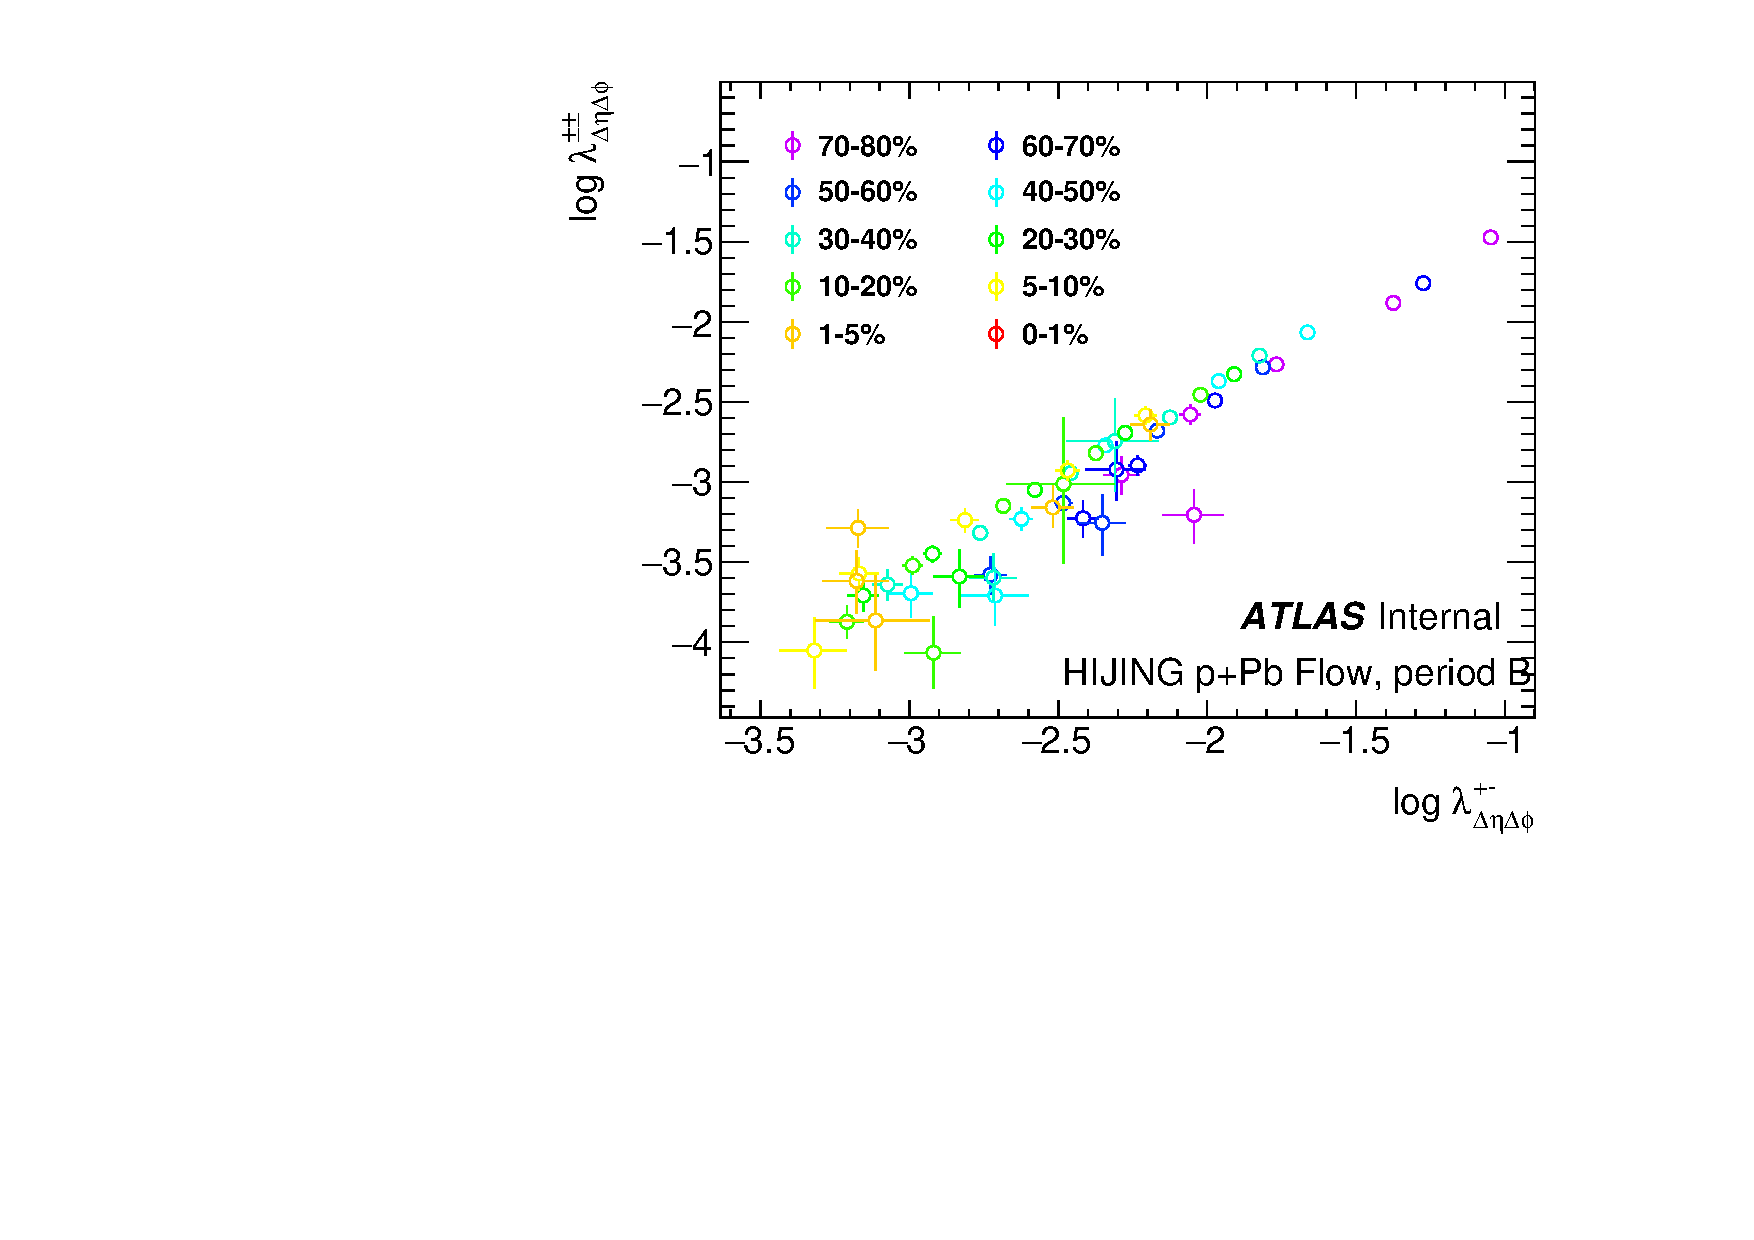
\includegraphics[width=.49\linewidth]{ang_lambda_opp_vs_same_MC.pdf}
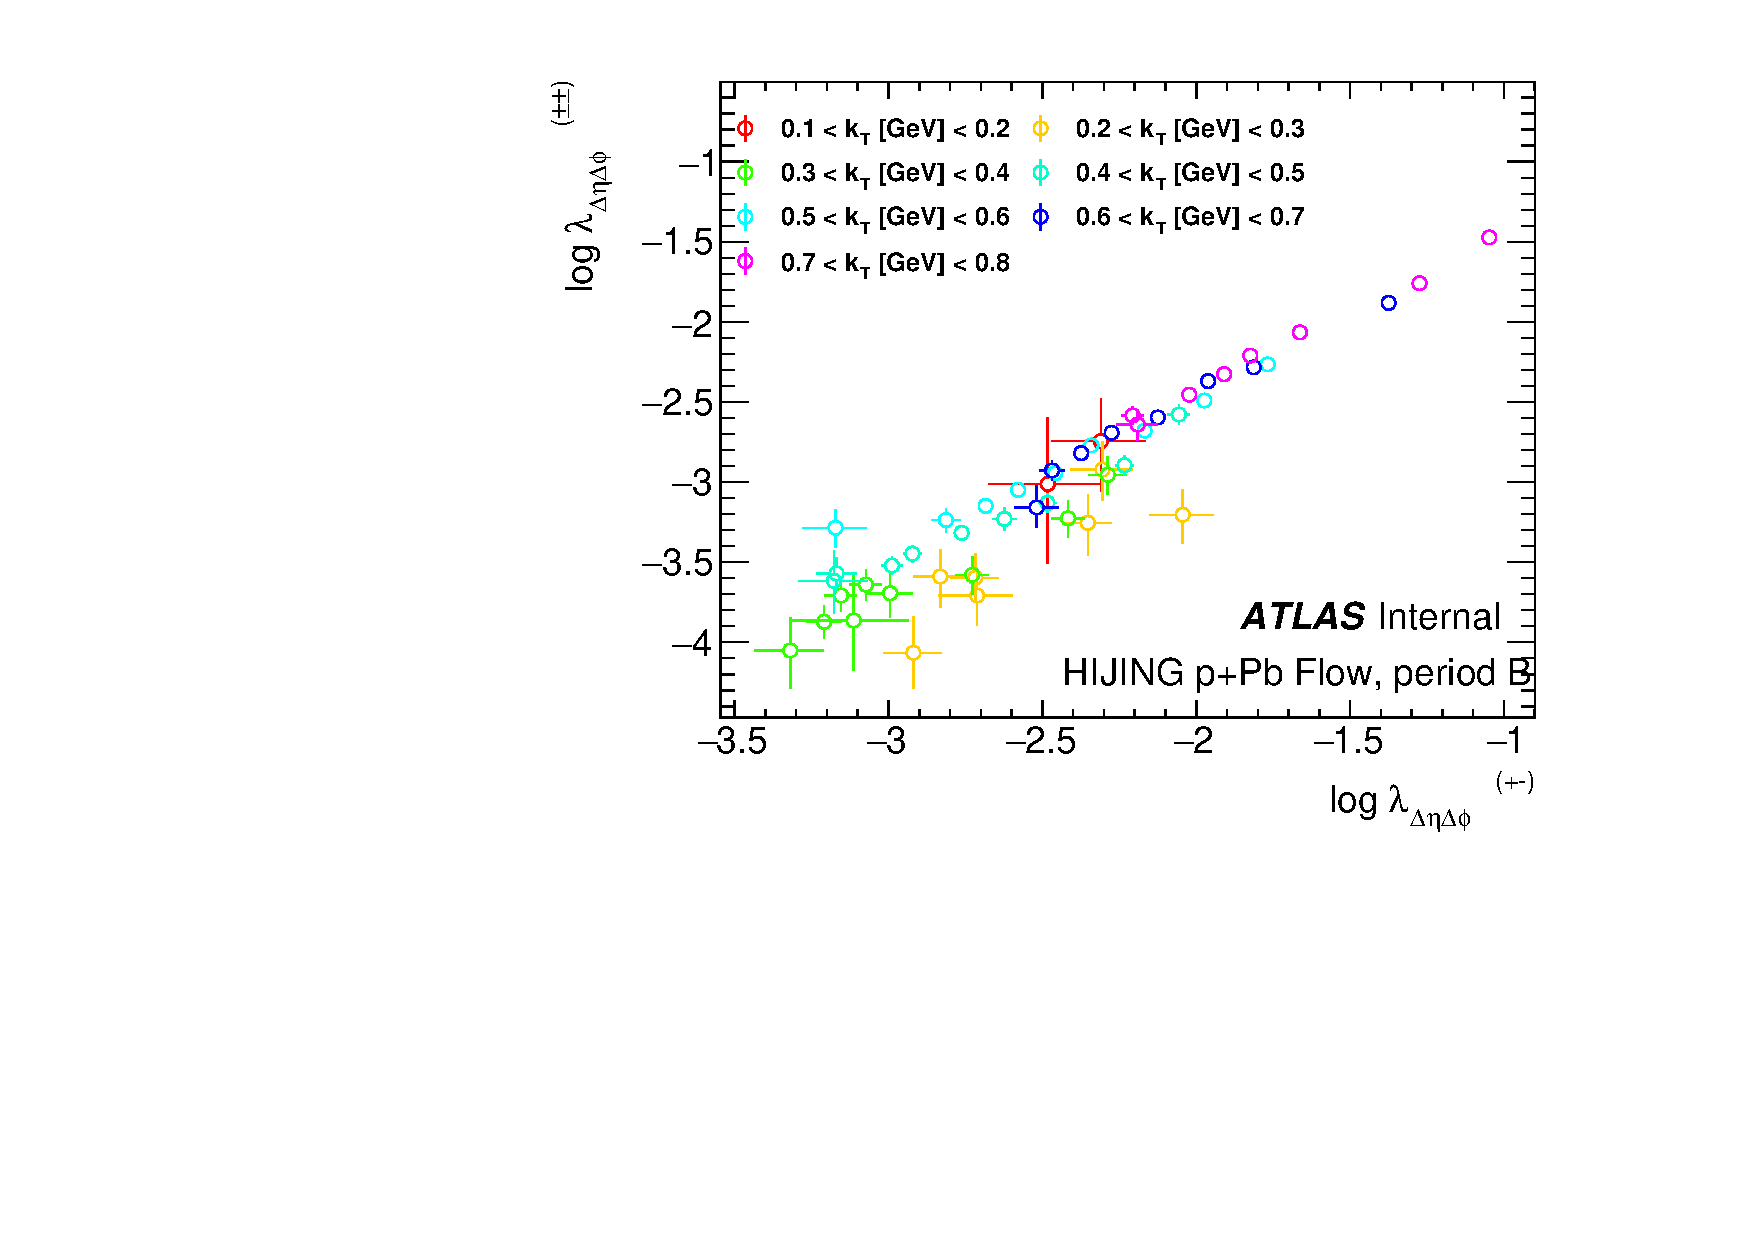
\includegraphics[width=.49\linewidth]{ang_lambda_kt_opp_vs_same_MC.pdf}
\caption{The amplitude of the jet contribution to $C(\Delta\eta, \Delta\phi)$ is largely correlated between like-sign and unlike-sign pairs. The plots are nearly identical, except that one is colored by centrality and the other by \kt. Some points have very large errors (with a sum of errors greater than 0.8) and are not shown.}
\label{fig:background_ang_same_vs_opp_mc}
\end{figure}

Rather than use a double-ratio, some femtoscopic analyses have described the background with one or more be a free fit parameter.
The results in this thesis use a data-driven method to tune it by comparing to opposite-sign pairs, Coulomb-corrected and with the largest resonance contributions removed, which do not have a Bose-Einstein correlation.
\Cref{fig:background_amp_inv_vs_ang_data}, which is taken from data, shows that the choice to tune from the amplitude of Gaussian fits to $\qinv$ or $\Delta\eta, \Delta\phi$ correlations does not significantly impact the result.
This further supports the interpretation that the enhancement in $\qinv$ comes from hard processes, as the peak in angular coordinates is commonly associated with jets.
\Cref{fig:background_ang_same_vs_opp_mc} shows the amplitudes of the jet contribution to $C(\Delta\eta, \Delta\phi)$ comparing both $++$ and $--$ to $+-$.
The correlation between $\pm\pm$ and $+-$ demonstrates that, at least in principle, the $+-$ correlation functions can constrain the hard-process contribution in $\pm\pm$ correlation functions.

Though some resonances are removed from the $+-$ correlation functions the effect of jet fragmentation is not identical in same-charge and opposite-charge.
The relationship between the two correlation functions is studied in \ac{MC} simulations so a mapping can be developed between $+-$ and $\pm\pm$.

To isolate the effect of jet fragmentation particles from weak decays ($\eta$, $\eta'$, and $\omega$) were excluded.
Pairs of particles from two-body resonance decays were also neglected in order to remove mass peaks in the correlation function.
The same pair mass cut around the $\rho$ resonance that is used in the data is applied in the \ac{MC}, since the removal of the corresponding region of phase space has a significant effect on the shape of the correlation function.

\FloatBarrier
\subsection{Monte Carlo generators}
\label{subsec:generators}

A number of Monte Carlo generators were utilized during studies of the non-\ac{HBT} part of the correlation function.
Detector simulation is not run on these samples.
In each of the following samples, 50 million (250 million for \PYEight) \minbias events are generated at a center of mass energy per nucleon of \pPbenergy.

\begin{enumerate}
\item \Hijing \pPb \cite{Gyulassy:1994ew}\\
  The energy and boost settings are the same as in the nominal \pPb reconstructed simulation, except that the minimum hard-scattering transverse momentum is adjusted as described above.
  Turning off the flow, which shifts the $\phi$ of particles in order to reproduce the flow harmonics $v_n$, was not found to have a significant effect on the momentum-space correlation functions.
  The minimum hard-scattering \pt parameter\footnote{HIPR18} is adjusted to show that the non-femtoscopic background originates from minijets, as described in \cref{fig:hard_process_min_pt}.

\item \Hijing \pp\\
  The simulation is run at $\sqrt{s} = 5 \TeV$ with all of the same settings as the \pPb sample, except that both incoming particles are protons.
  No rapidity boost is applied because the collision system is symmetric.

\item \Pythia 8.2 \pp \cite{Sjostrand:2007gs}\\
The default ATLAS tune "UE AU2-CTEQ6L1" is used with \PYEight at $\sqrt{s} = 5.02 \TeV$.
This utilizes the CTEQ 6L1 \ac{PDF} from LHAPDF6 \cite{Buckley:2014ana}.

\item \Herwig++ 2.7 \pp \cite{Bahr:2008pv}\\
A known bug in \Herwig++ 2.7.1 prevented the use of the CTEQ6 \ac{PDF}, so the default MRST \ac{PDF} was used instead.
This should not be a significant issue for these purposes, because the jet fragmentation is not very dependent on the initial state.

It should be noted that the correlation functions predicted by \Herwig are in such significant and obvious disagreement with those seen in the data that they cannot be used directly.
The \Herwig sample is used to compare the variation of certain behavior of the correlation functions compared to \Pythia in order to establish an estimate for the systematic uncertainty arising from the details of the generator (as will be described in \cref{subsec:herwig_vs_pythia}).
\end{enumerate}


\subsection{Jet fragmentation in Lorentz invariant correlation function}
\label{subsec:jet_frag_inv}

In order to describe the background satisfactorily it is necessary to loosen the assumption of a Gaussian form in \qinv.
The \qinv correlation functions in \PYEight were fit to
\begin{equation}
  \label{eq:jet_frag_form_inv}
  \Omega(\qinv) = 1 + \lbkgd e^{-|\Rbkgd \qinv|^{\abkgd}}
\end{equation}
The results are shown in \cref{fig:background_alpha_pythia8,fig:background_qinv_same_vs_opp_pythia8}.

\begin{figure}[t]
\centering
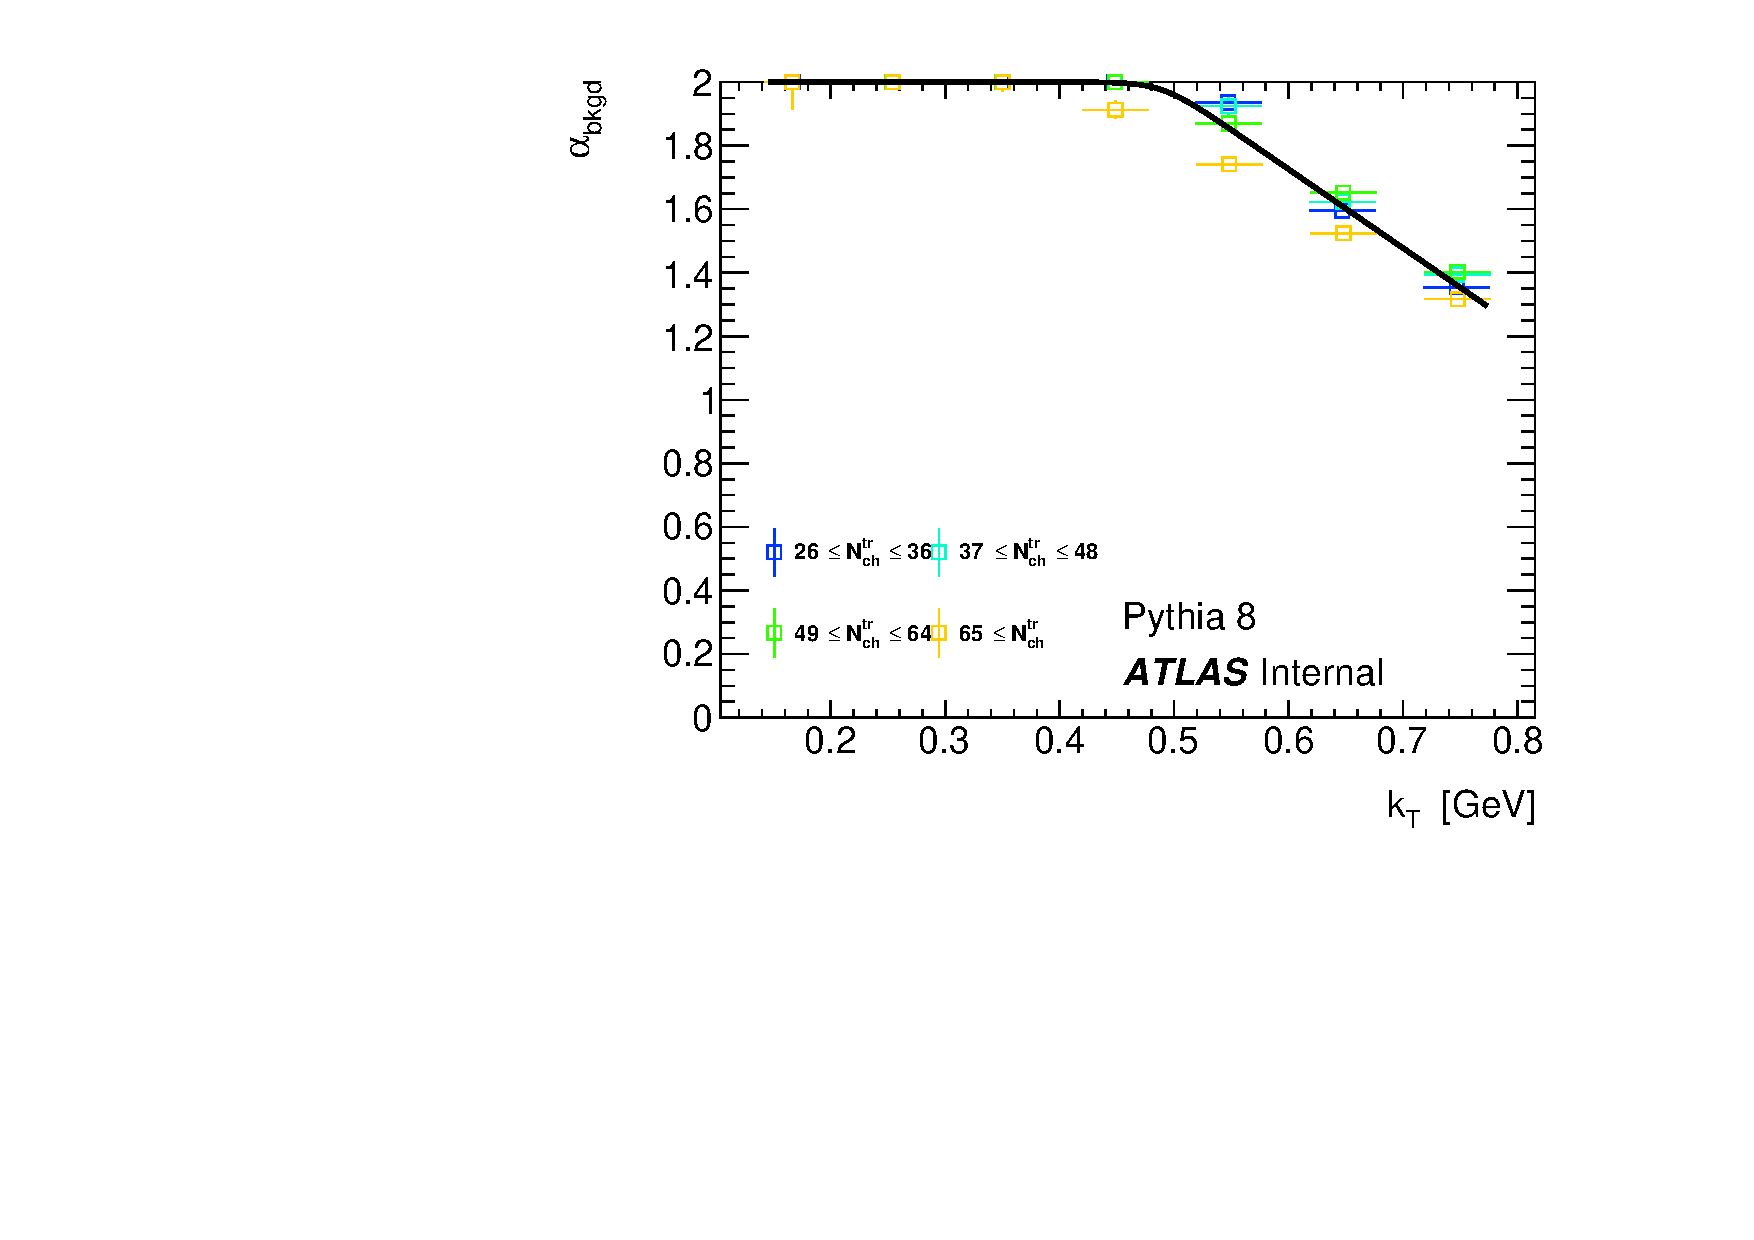
\includegraphics{qinv_backAlpha_vs_kt_pythia8.pdf}
\caption{The tail weight parameter \abkgd of fits to $C^{\pm\pm}(\qinv)$ as a function of \kt in \PYEight, in four multiplicity bins. \abkgd is limited by above at 2 (the Gaussian case), and for low \kt bins this is sufficient to describe the background shape. The parameter is fit to a function of the form $\abkgd = 2 - 0.0497 \log \left(1 + e^{50.9(\kt - 0.493)} \right)$, with \kt in GeV.
}
\label{fig:background_alpha_pythia8}
\end{figure}

\begin{figure}[t]
\centering
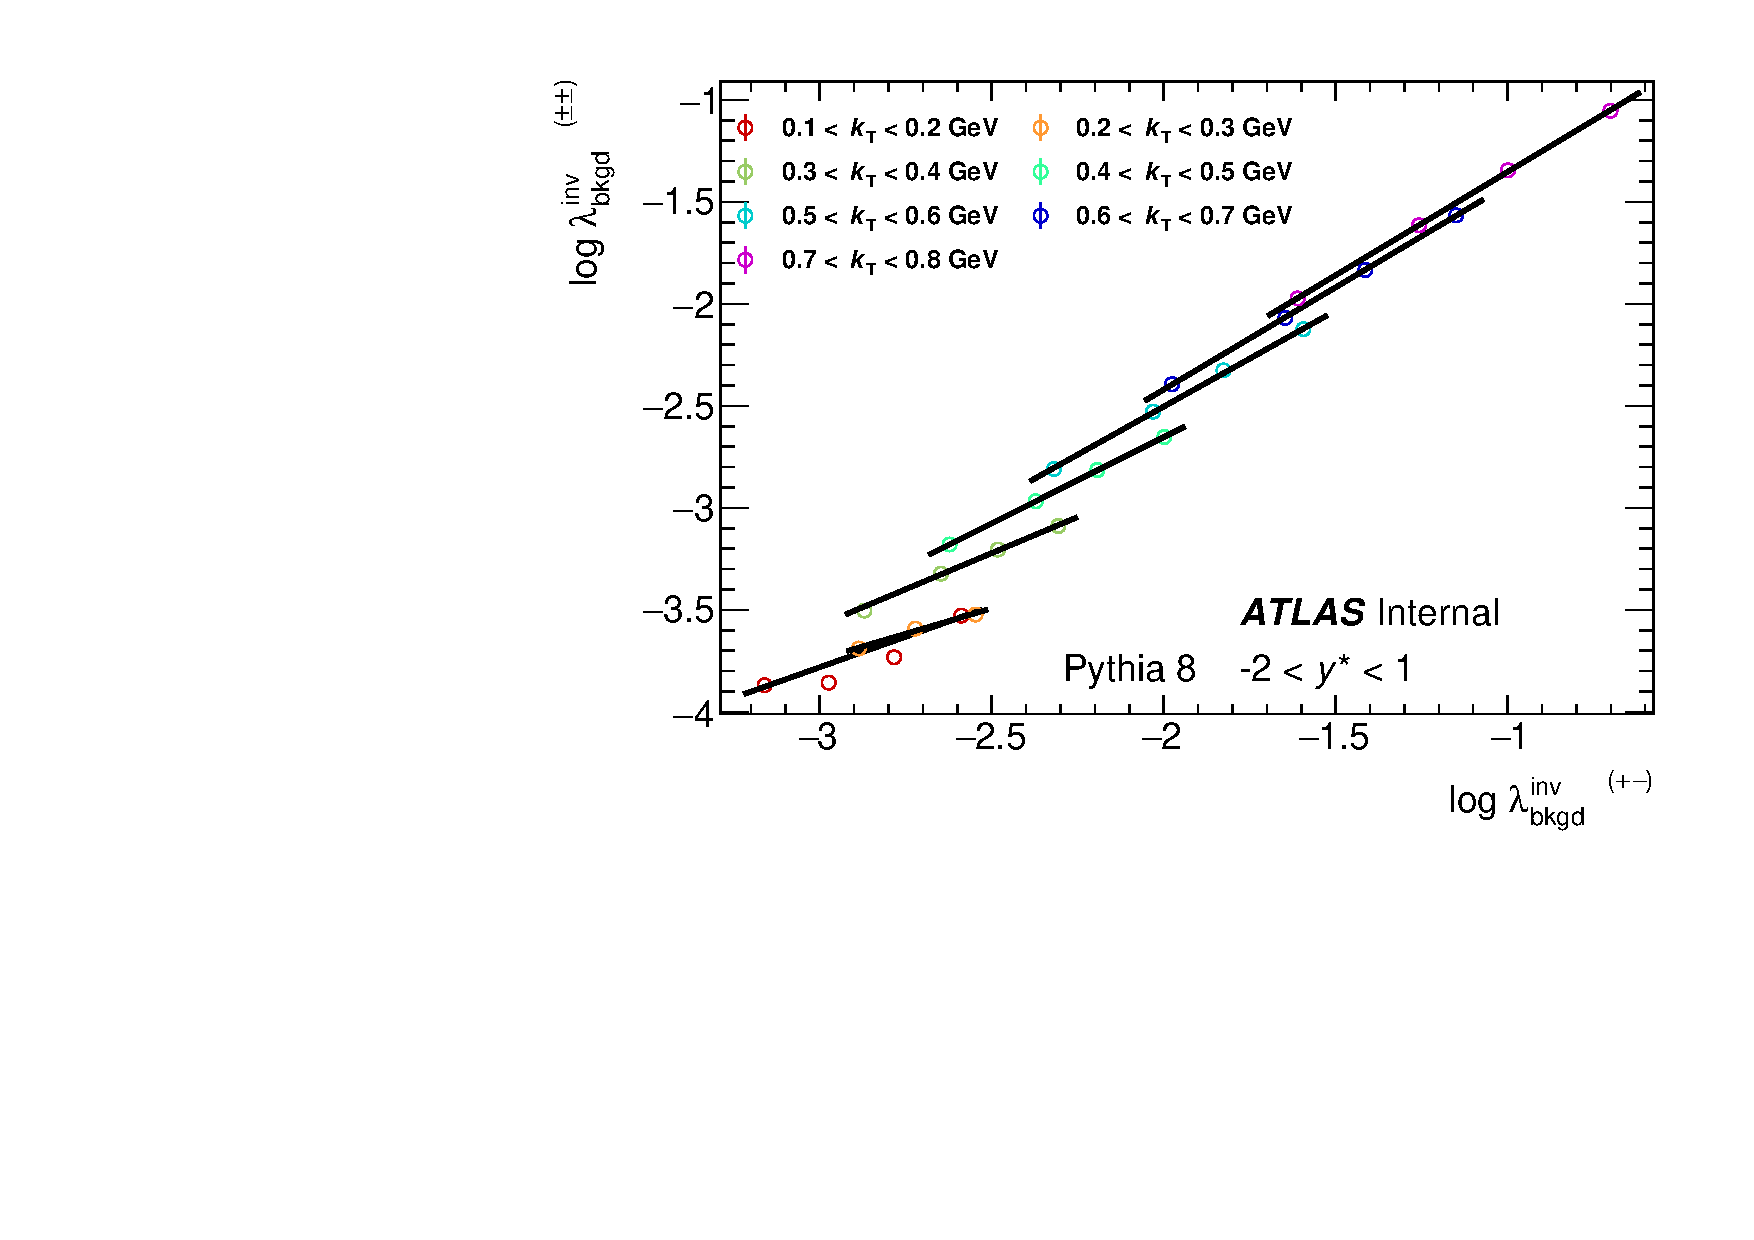
\includegraphics[width=.49\linewidth]{qinv_pythia8_backLambda_kt_opp_vs_same.pdf}
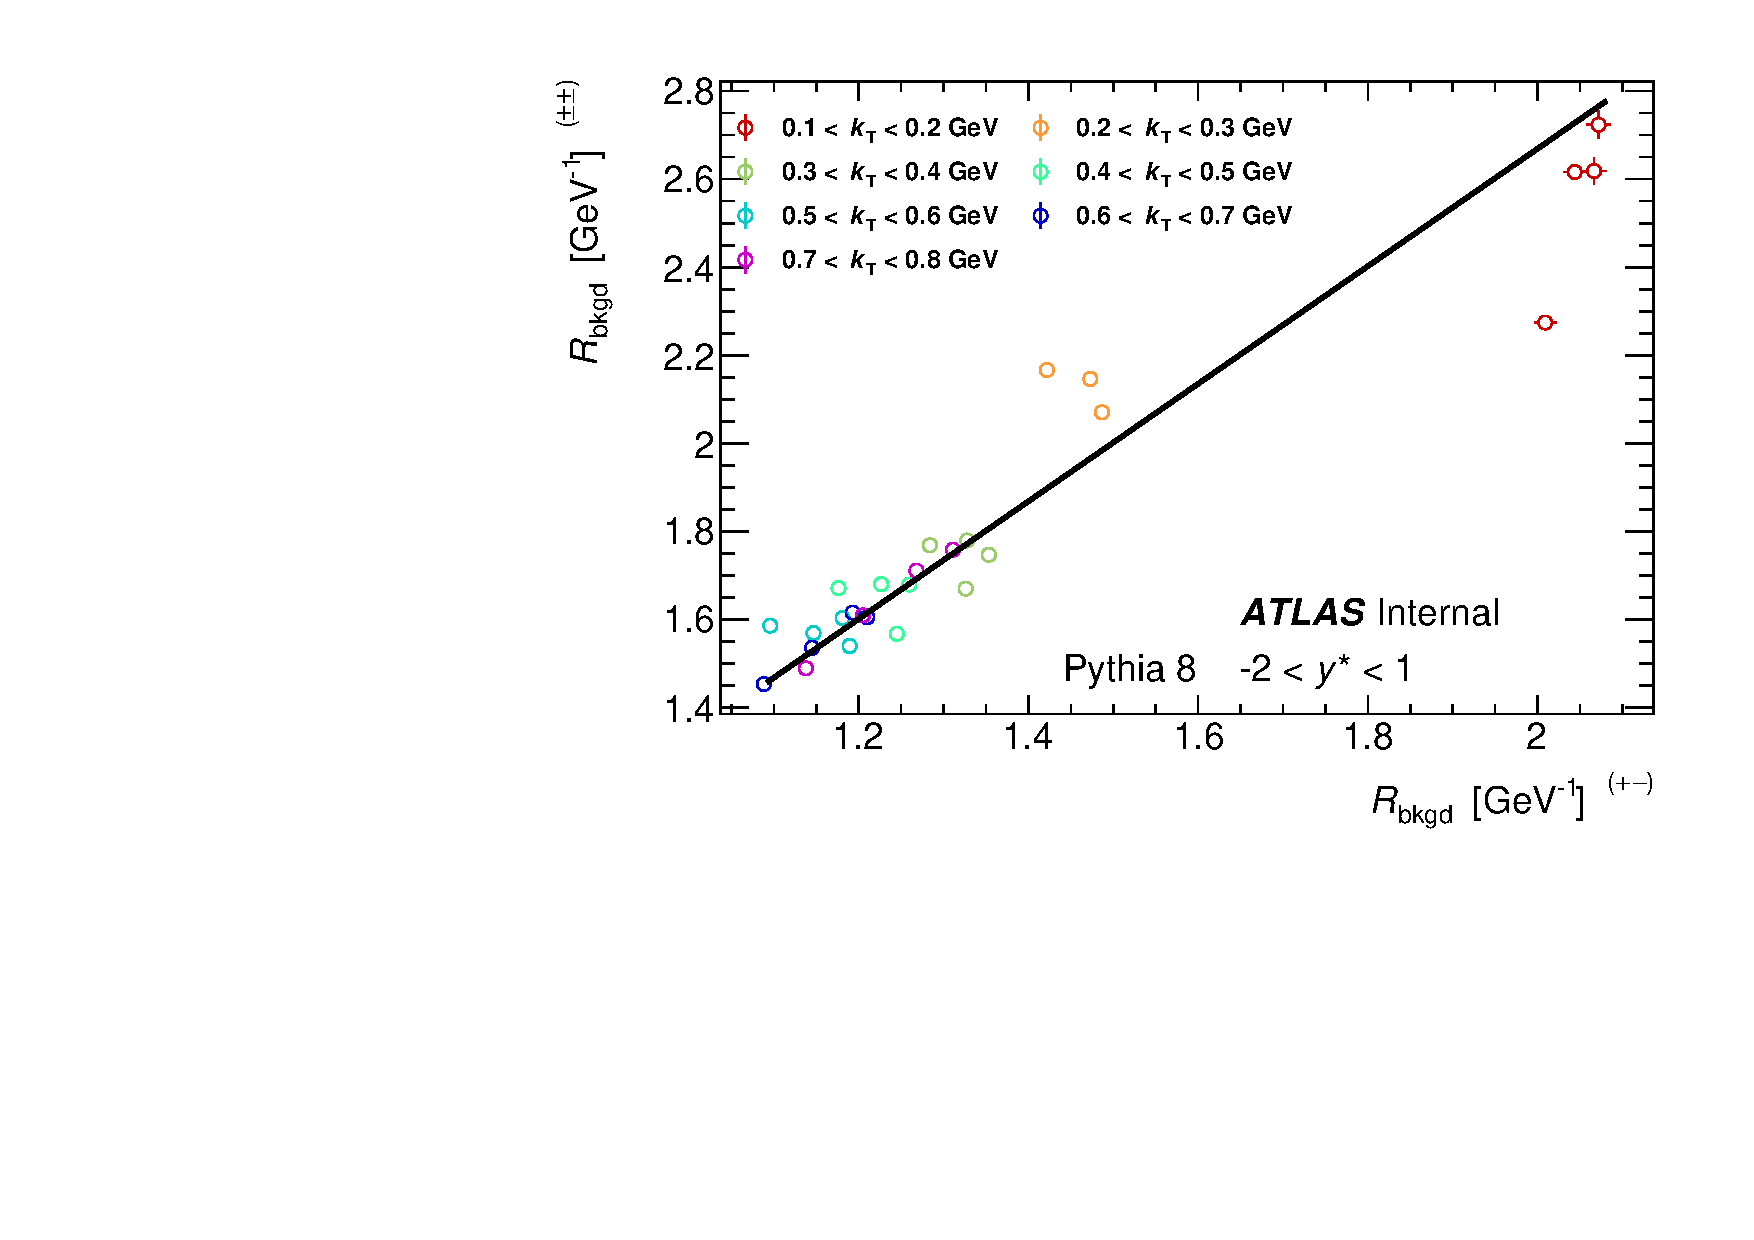
\includegraphics[width=.49\linewidth]{qinv_pythia8_backR_kt_opp_vs_same.pdf}
\caption{A comparison of same-sign to opposite-sign charged pairs with the amplitude and width of $\alpha$-stable fits in \PYEight. Several multiplicities are shown in each colored \kt bin, with the multiplicity bins defined in \cref{fig:background_alpha_pythia8}, and the $++$ and $--$ pairs are separated. The slopes and intercepts of the lines in the left plot are shown in \cref{fig:background_qinv_same_vs_opp_pythia8_fits}. The widths $\Rbkgd$ are fit to a simple ratio $\rho$ from \cref{eq:rho}. In the amplitude plot (left), the widths $\Rbkgd$ are fixed to the value extracted from the right plot.}
\label{fig:background_qinv_same_vs_opp_pythia8}
\end{figure}

\begin{figure}[t]
\begin{minipage}[t]{1.0\textwidth}
\centering
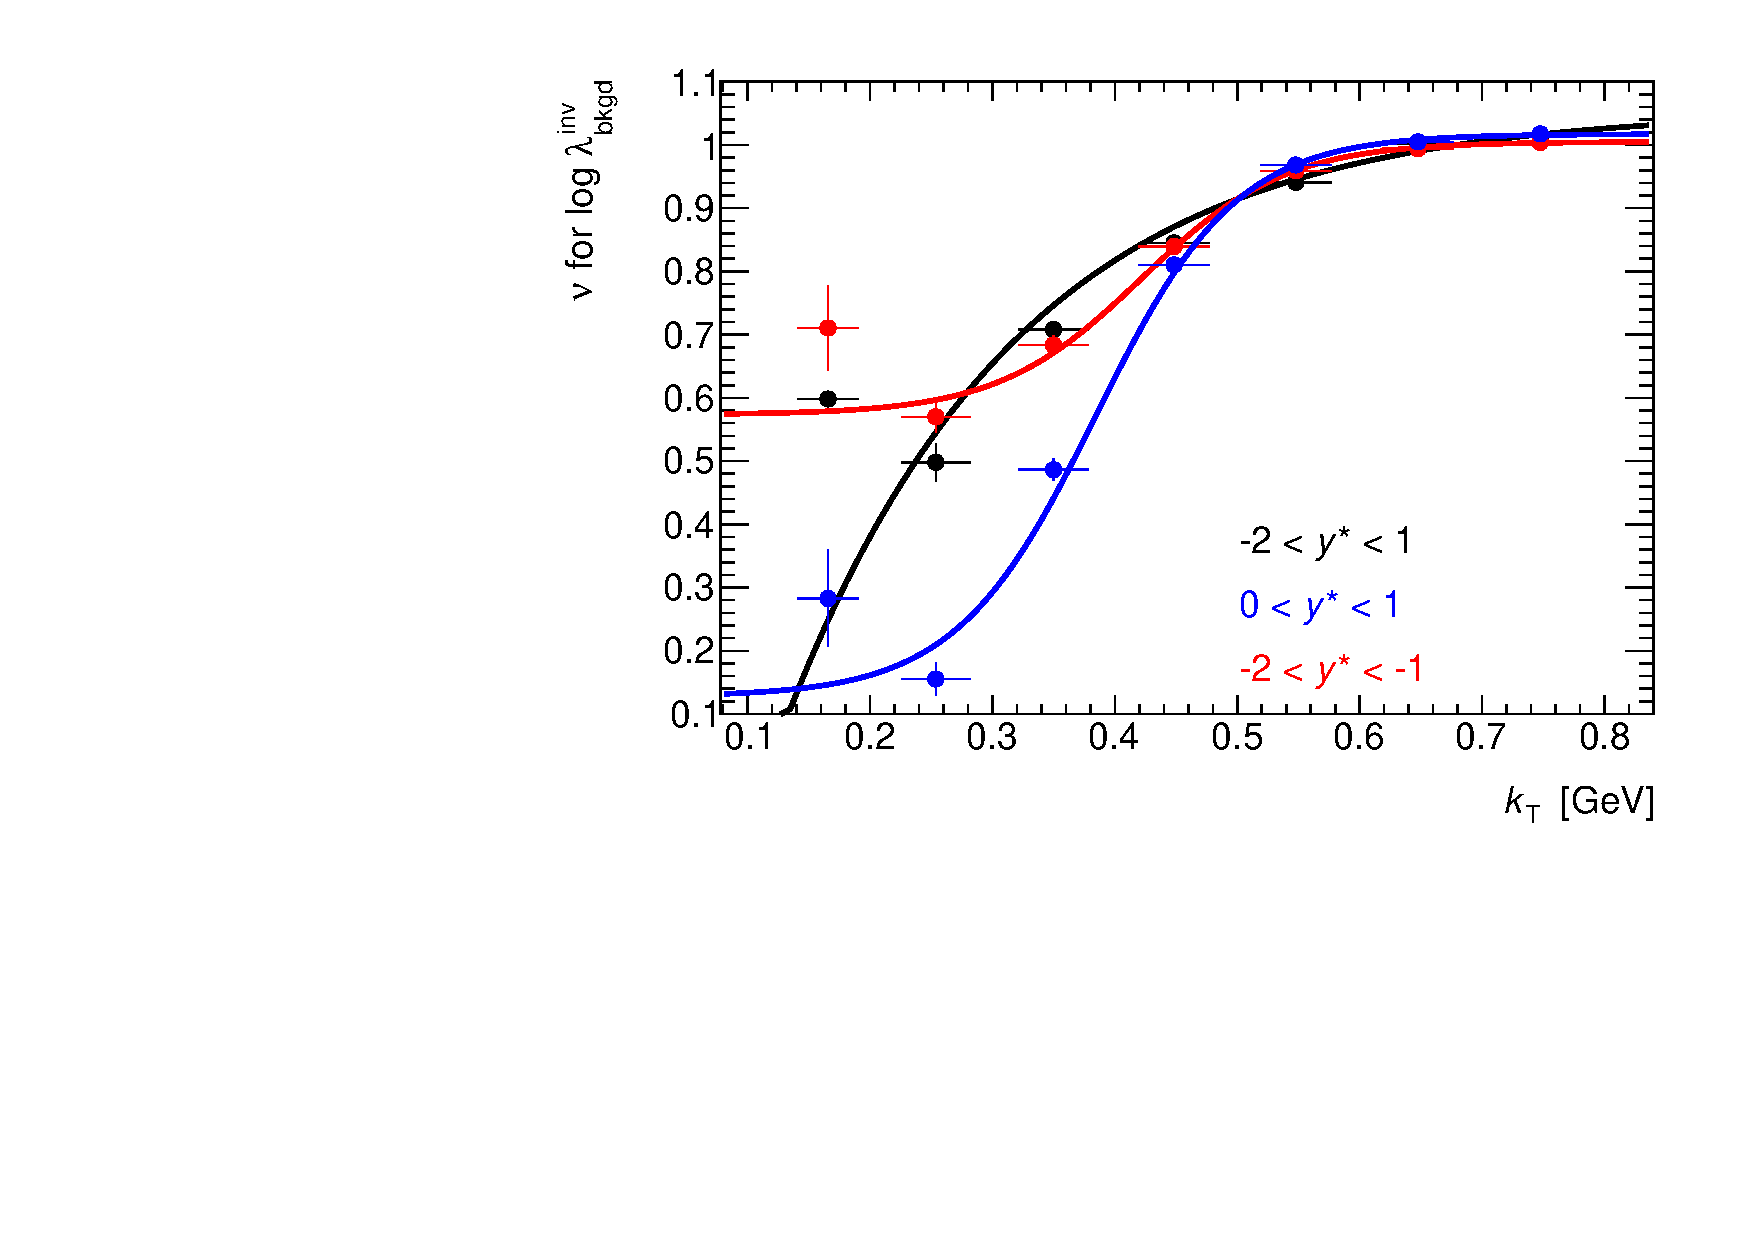
\includegraphics[width=.49\linewidth]{can_kt_qinv_backLambda_slope_combined.pdf}
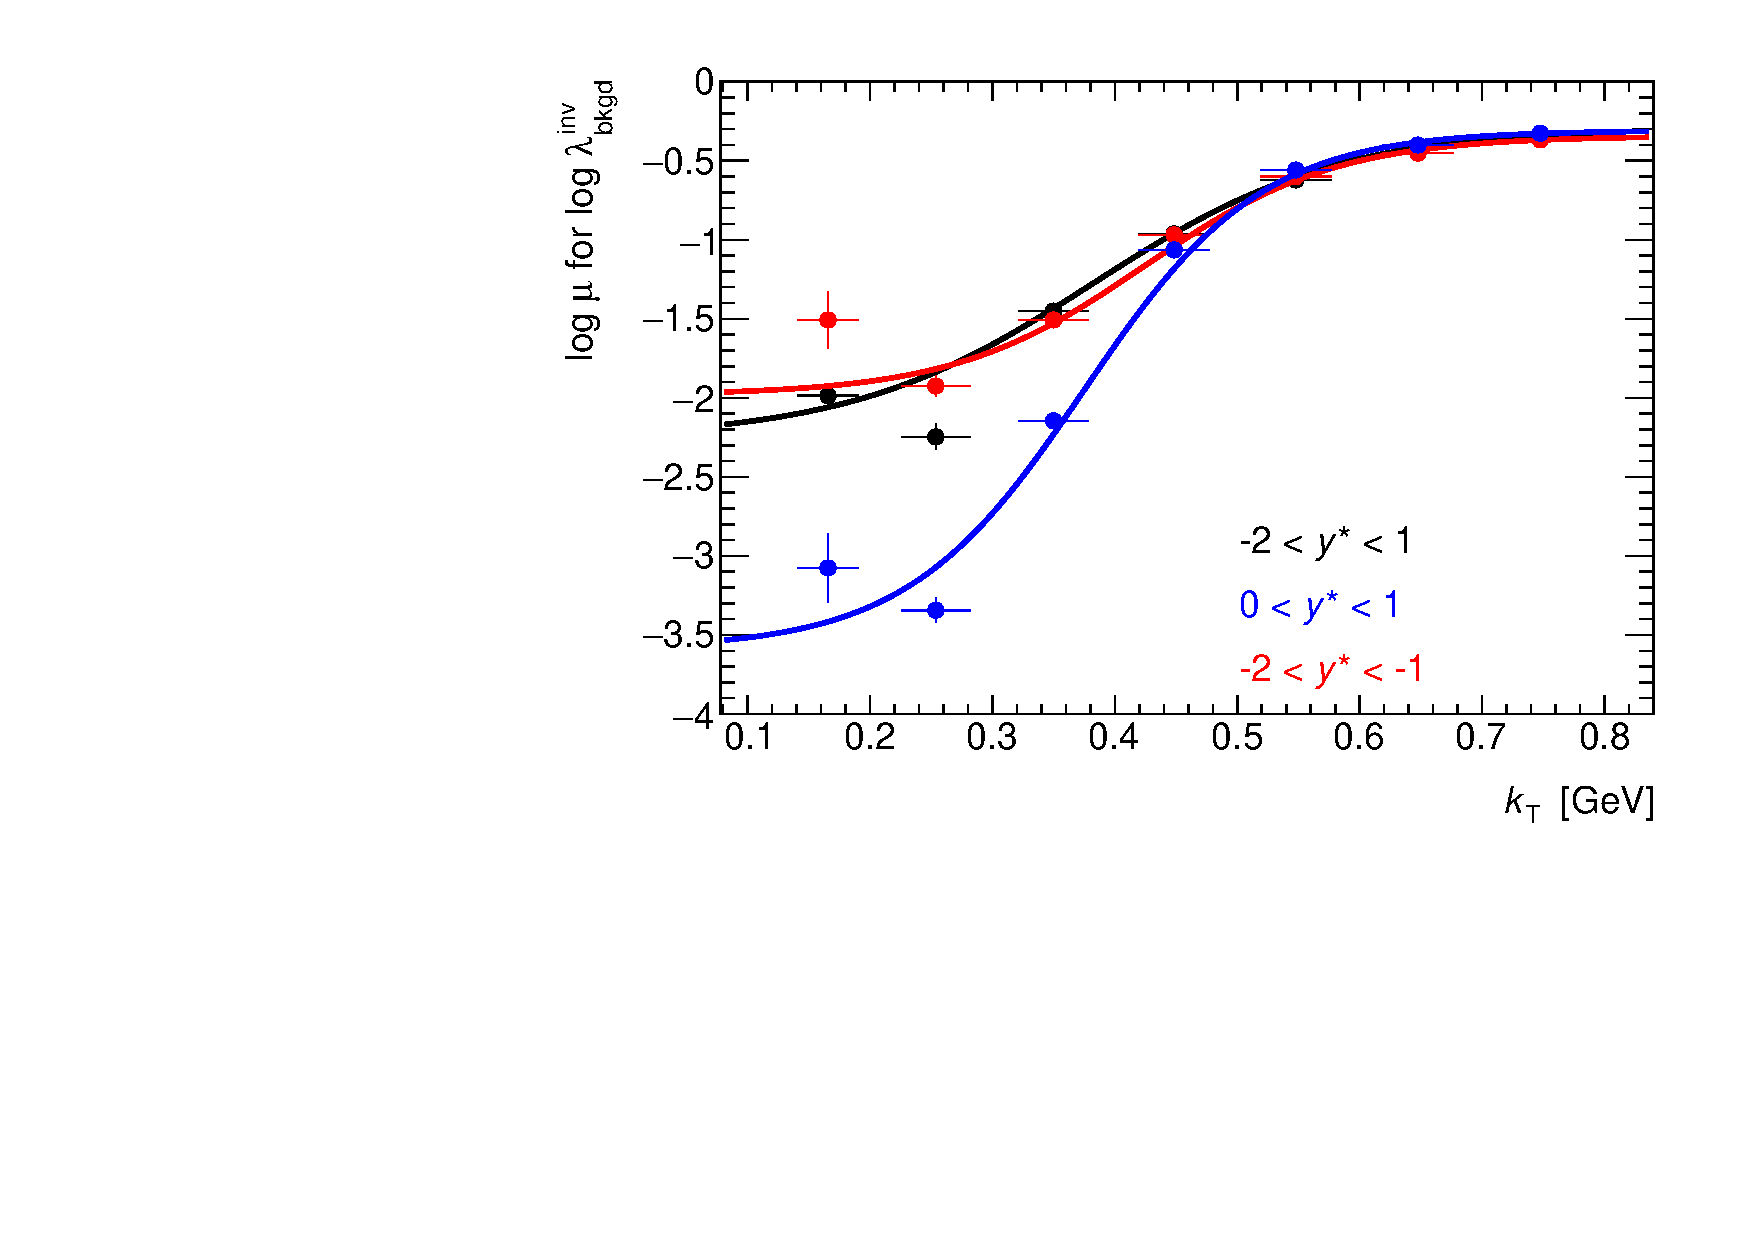
\includegraphics[width=.49\linewidth]{can_kt_qinv_backLambda_intercept_combined.pdf}
\end{minipage}
\caption{The slopes (left) and intercepts (right) of the fits from \cref{fig:background_qinv_same_vs_opp_pythia8} as defined in \cref{eq:lambdaBackPar}. The parameters are each fitted to a function of the form $p_1 + \frac{p_2}{1 + e^{-p_3(k_T - p_4)}}$. The results of the fits are displayed in \cref{eq:mu,eq:nu}. The procedure is perfomed in both forward (red) and central (blue) rapidity bins, and the results are used as a systematic variation.}
\label{fig:background_qinv_same_vs_opp_pythia8_fits}
\end{figure}

In one attempt to constrain the background, correlation functions were generated in \PYEight (which does not have Bose-Einstein or Coulomb effects) and the width and height of the correlation functions were compared from like-sign to unlike-sign.
\cref{fig:background_qinv_same_vs_opp_pythia8} shows the comparison for each \kt bin for a few choices of multiplicity ($26 \leq \Nch^{tr} \leq 36$, $37 \leq \Nch^{tr} \leq 48$, $49 \leq \Nch^{tr} \leq64$, $65 \leq \Nch^{tr}$).
The amplitudes are compared on a log scale and straight lines are fit for each \kt bin.
The widths $\Rbkgd^{\pm\pm}$ and $\Rbkgd^{+-}$ are taken to be proportional to each other by a constant factor.
This assumption is clearly not perfect but becomes increasingly accurate at high \kt, where the background contribution is largest.

This \kt dependence of fit parameters is used as a mapping from opposite-sign fits in the data to a fixed background gaussian.
In summary we are requiring that

\begin{align}
\lbkgd^{\pm\pm} &= \mu(\kt) \left(\lbkgd^{+-}\right)^{\nu(\kt)} \label{eq:lambdaBackPar}\\
\Rbkgd^{\pm\pm} &= \rho \Rbkgd^{+-} \label{eq:rBackPar}
\end{align}

and fixing $\mu(k_T)$, $\nu(k_T)$, and $\rho$ from the Monte Carlo with the results shown in \cref{fig:background_qinv_same_vs_opp_pythia8_fits}:

\begin{align}
\log \mu (\kt [\textrm{GeV}]) &= -2.26 + \frac{1.97}{1 + e^{-10.1 (\kt - 0.383)}} \label{eq:mu}\\
\nu(\kt [\textrm{GeV}]) &= 0.579 + \frac{4.38}{1 + e^{-14.4 (\kt - 0.425)}} \label{eq:nu}\\
\rho &= 1.33 \label{eq:rho} %% this constant is independent over rapidity to within ~2%
\end{align}
The statistical errors on the above parameters are on the order of 10\%.


\subsection{Jet fragmentation in three dimensions}
\label{subsec:jet_frag_3d}

In the longitudinally co-moving frame of a particle pair produced in a jet, on averate the axis of the jet will be aligned with the ``out'' direction and the plane transverse to the jet's momentum will be spanned by the ``side'' and ``long'' directions. In three dimensions the correlation from jet fragmentation is factorized into components which separately describe the ``out'' direction and both the ``side'' and ``long'' directions:
\begin{equation}
\Omega(\mathbf{q}) = 1 + \lbkgd^\mathrm{osl} \exp\left(-\left| R_\mathrm{bkgd}^\mathrm{out} \qout \right|^{\abkgd^\mathrm{out}} - \left| R_\mathrm{bkgd}^\mathrm{sl} \qsl \right|^{\abkgd^\mathrm{sl}}\right) \label{eq:jet_frag_form_3d}
\end{equation}
with $\qsl = \sqrt{\qside^2 + \qlong^2}$.
The shape parameters $\abkgd^\mathrm{out}$ and $\abkgd^\mathrm{sl}$ are fixed to 1.5 and 1.7 respectively, as shown in \cref{fig:pythia_bkgd_alpha}.
These parameters are not statistically consistent with constants independent of \kt and multiplicity.
However, at larger \kt, where the jet fragmentation is significant, the values do not vary enough to change the shape of the function drastically.
What is lost in precision is gained in the utility of having good control over the remaining parameters.
A systematic check is performed to investigate the effect of the shape on the results, and the results are seen to be insensitive at the 1\% level to variations of 0.1 in the \abkgd parameters.

\begin{figure}[t]
\centering
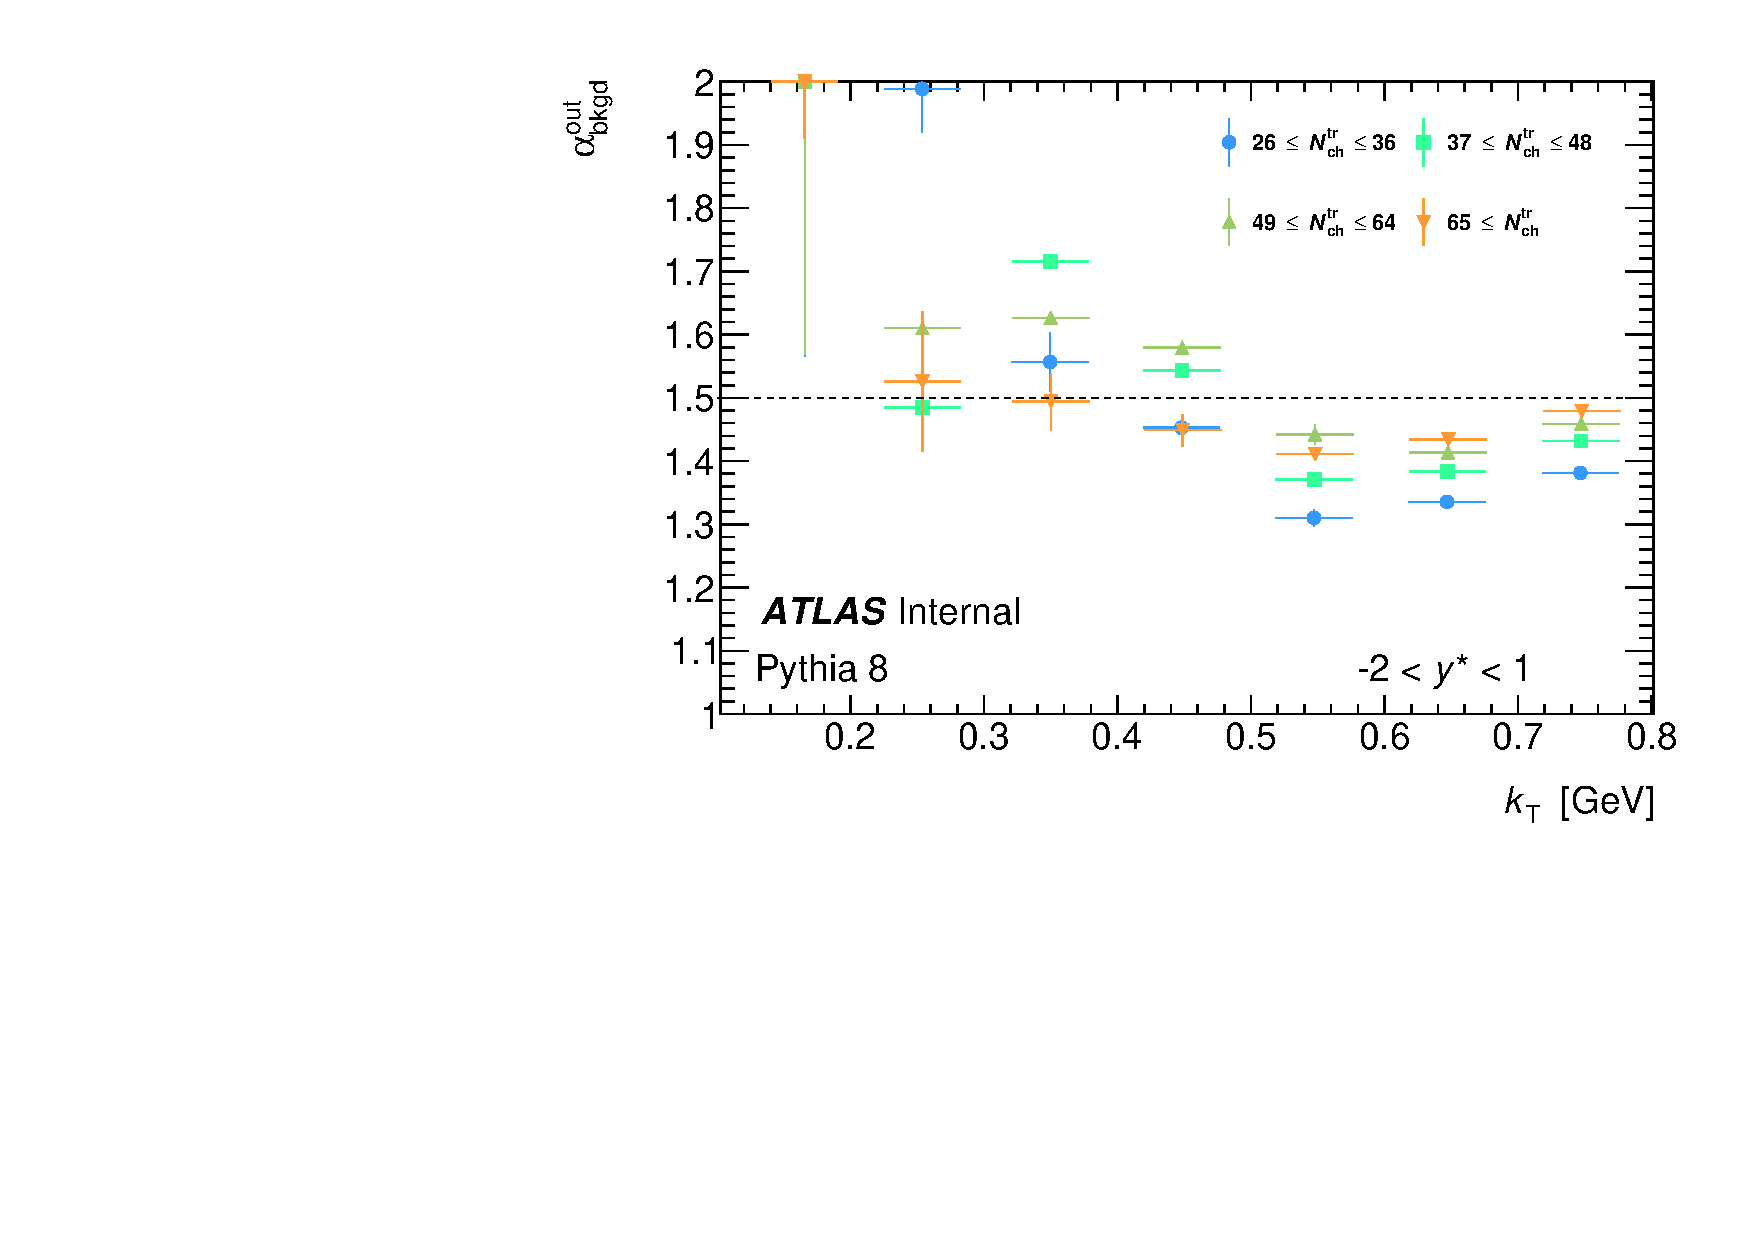
\includegraphics[width=.49\linewidth]{canqosl_backAlphaOut_vs_kt.pdf}
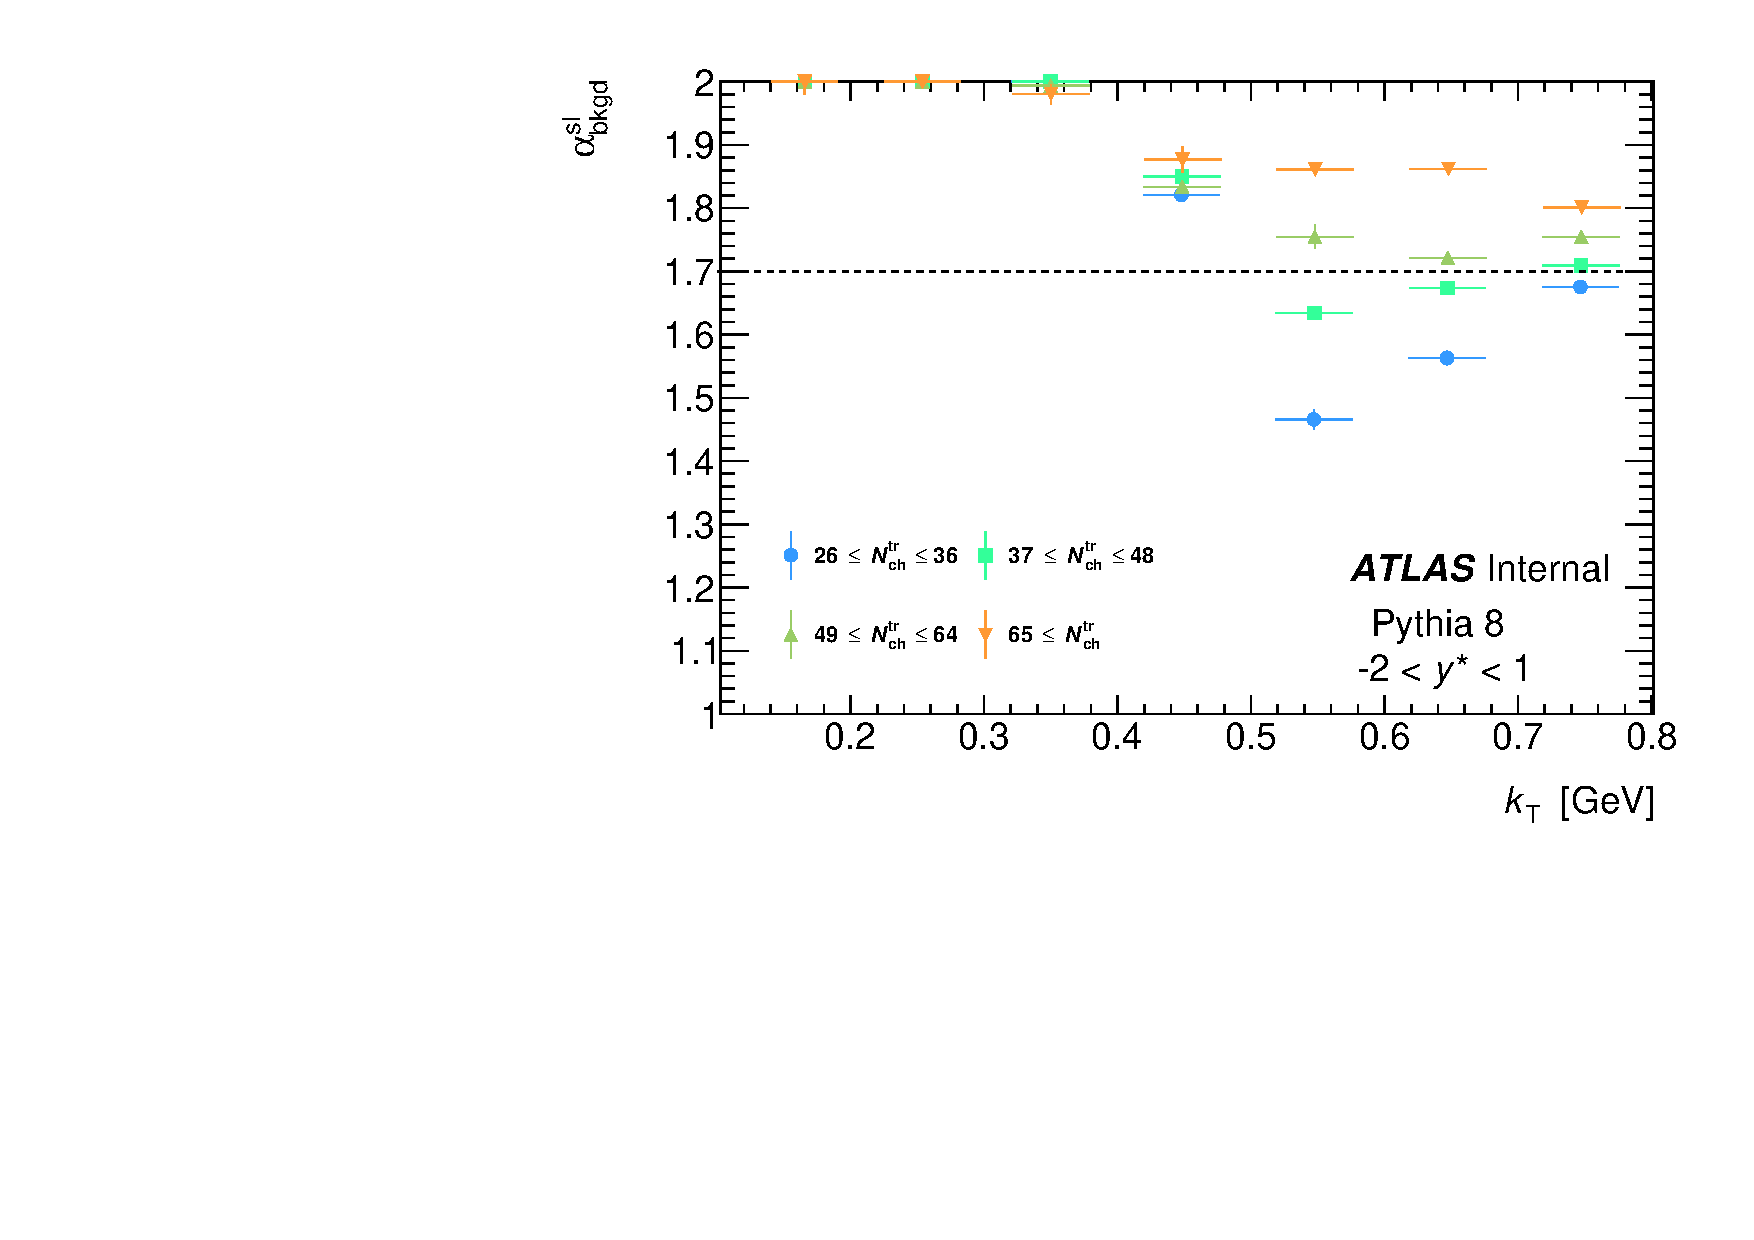
\includegraphics[width=.49\linewidth]{canqosl_backAlpha_vs_kt.pdf}\\
\caption{The fit results from \PYEight of the shape parameters from \cref{eq:jet_frag_form_3d}. The dashed lines indicate the constant values used in the analysis. While the results are not well-described by a constant function, the difference in the shape of the function is not extreme over the discrepancies observed.}
\label{fig:pythia_bkgd_alpha}
\end{figure}


\begin{figure}[t]
\begin{minipage}[t]{1.0\textwidth}
\centering
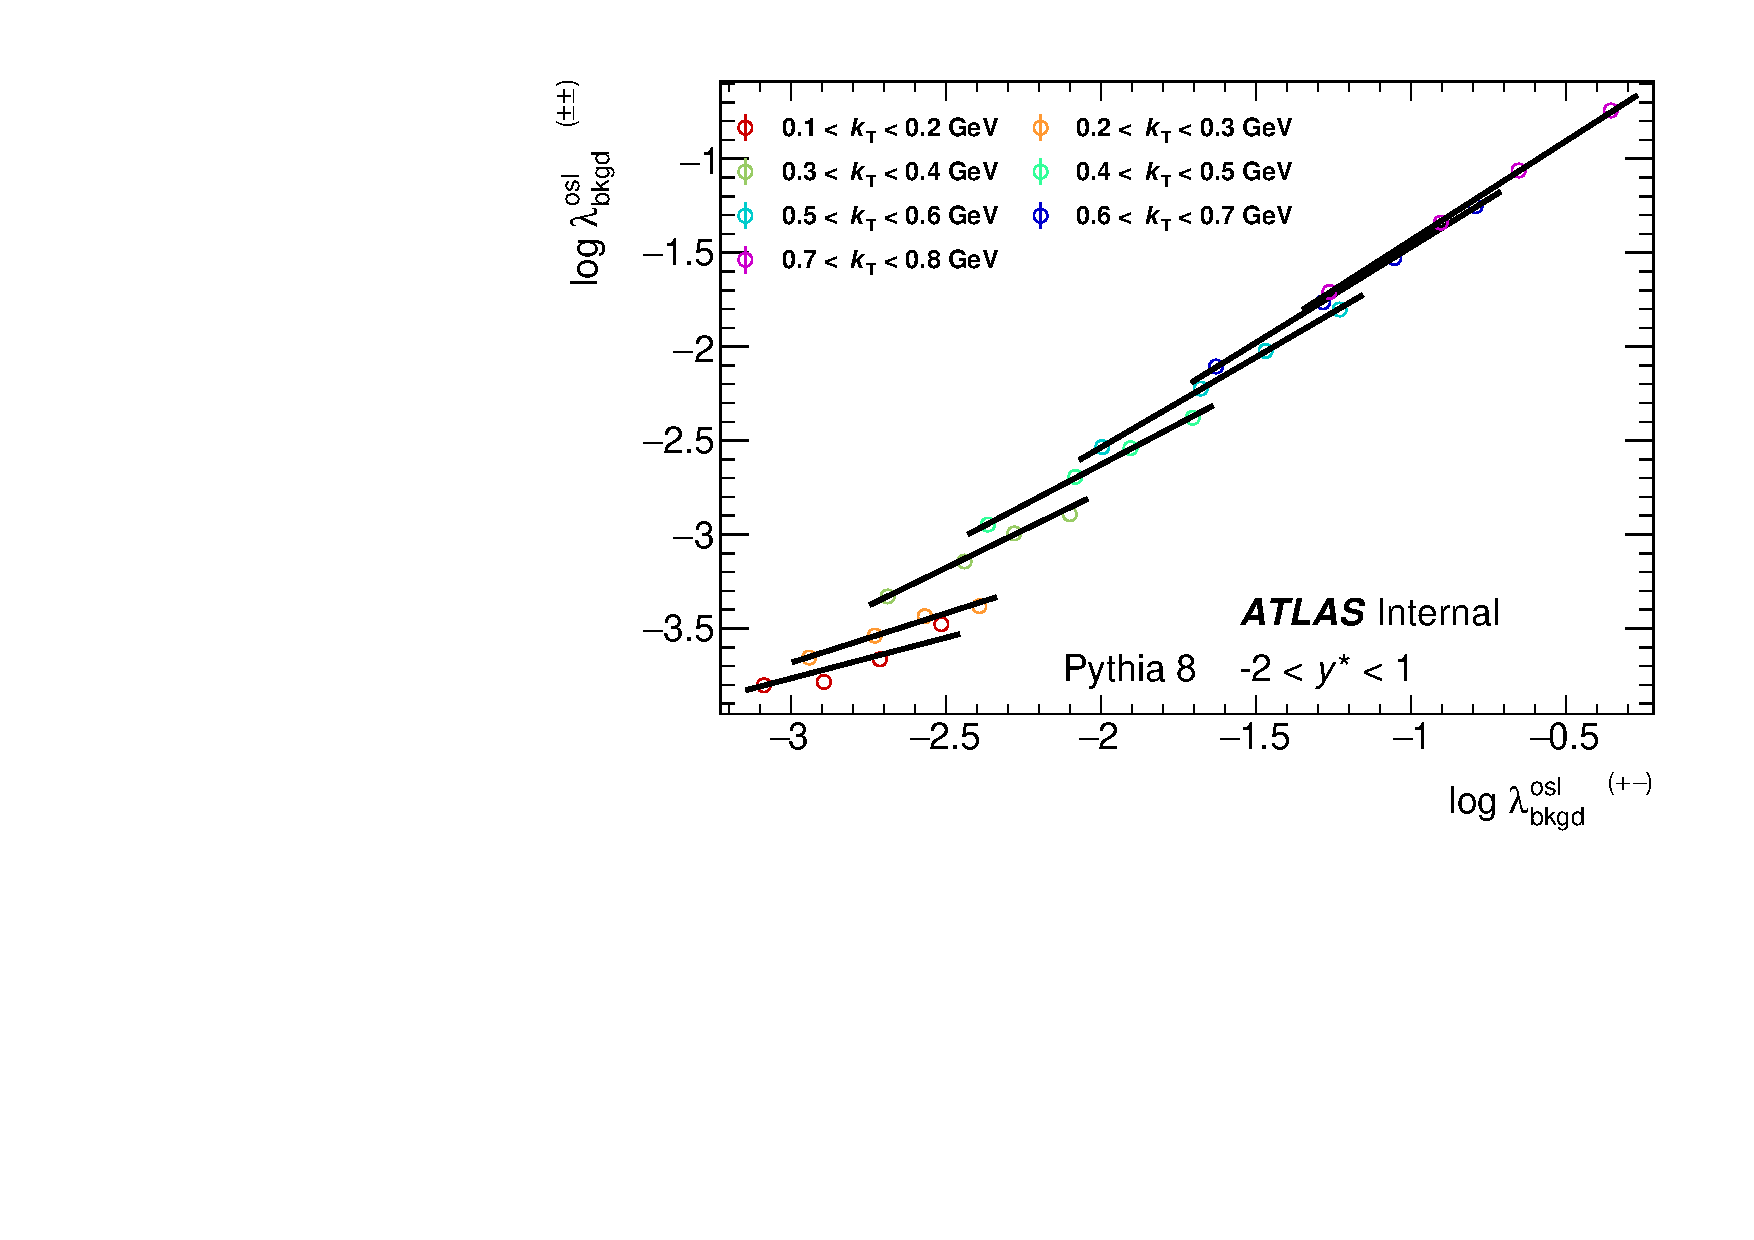
\includegraphics{can_kt_qosl_backLambda.pdf}\\
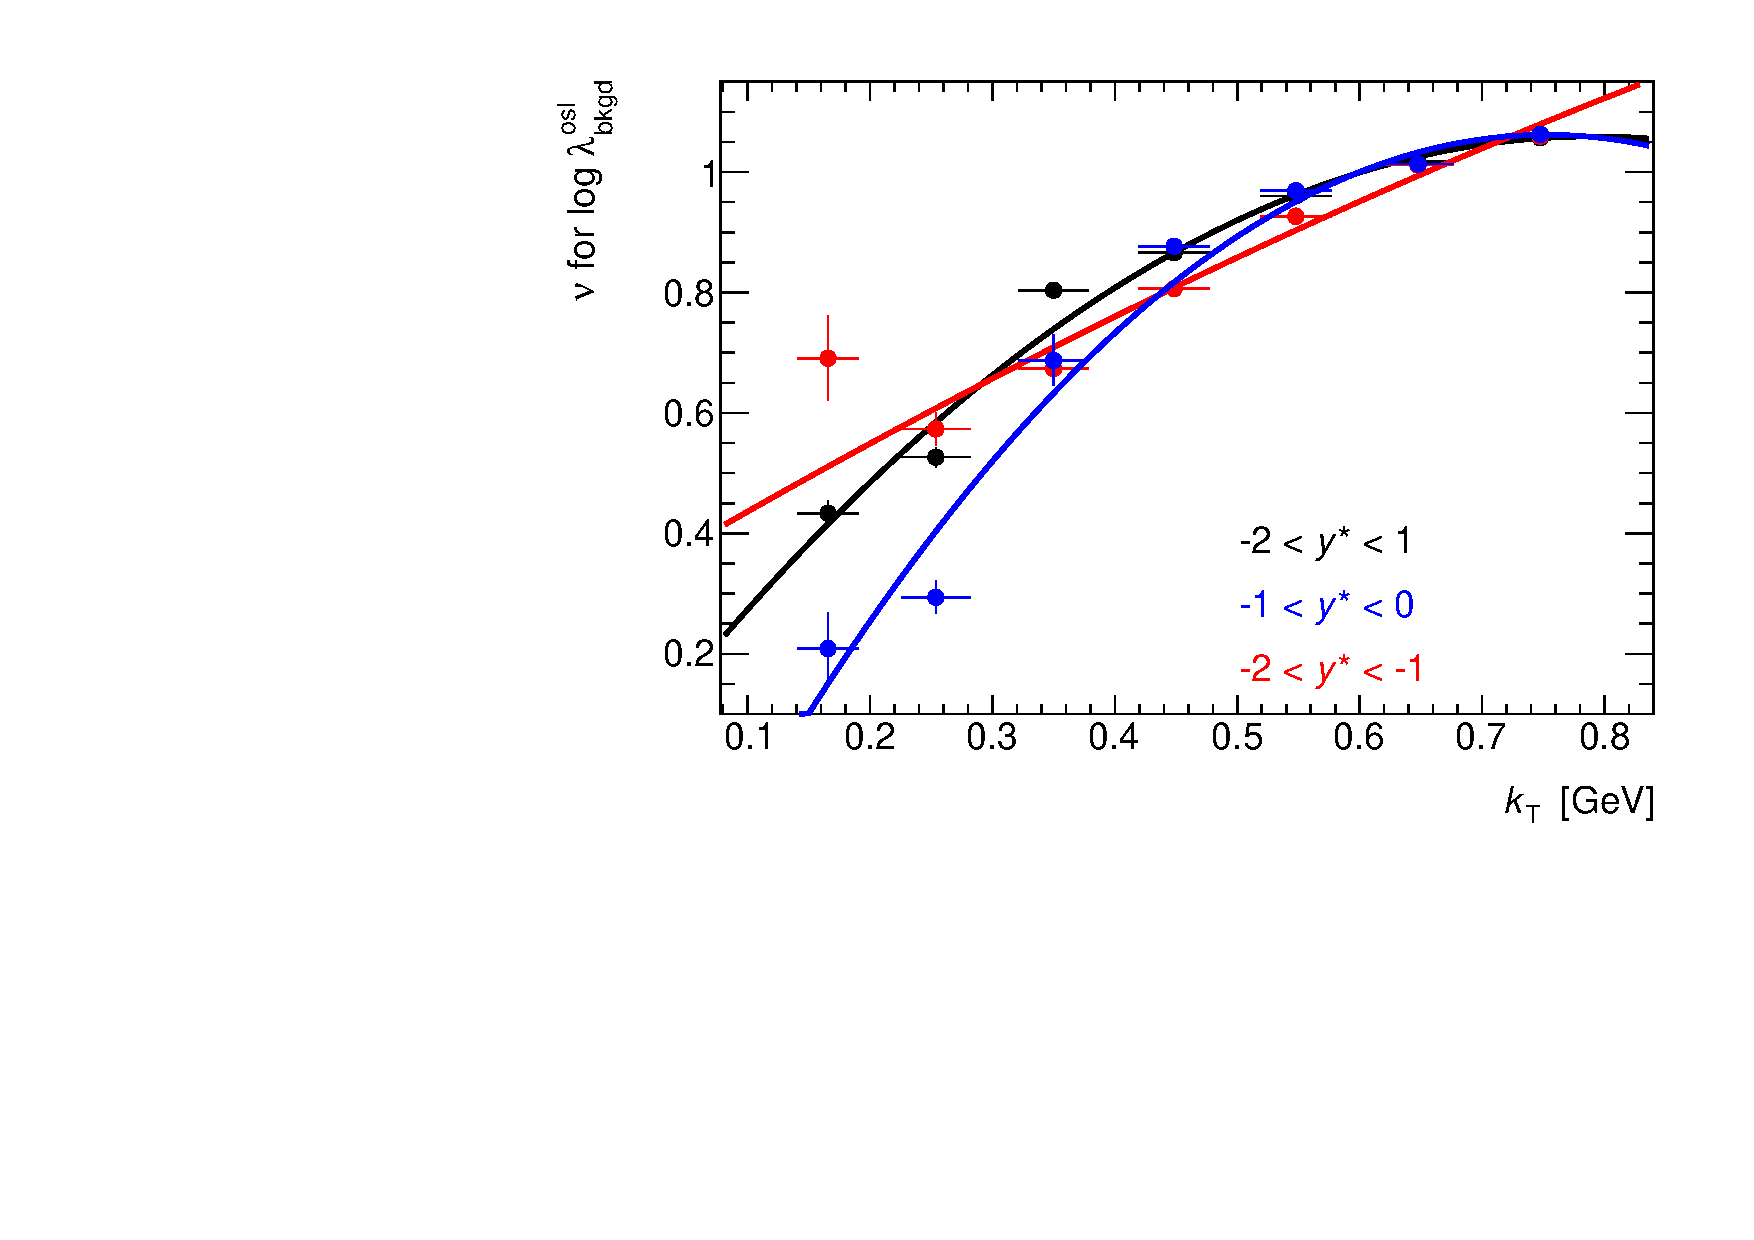
\includegraphics[width=.49\linewidth]{can_kt_qosl_backLambda_slope_combined.pdf}
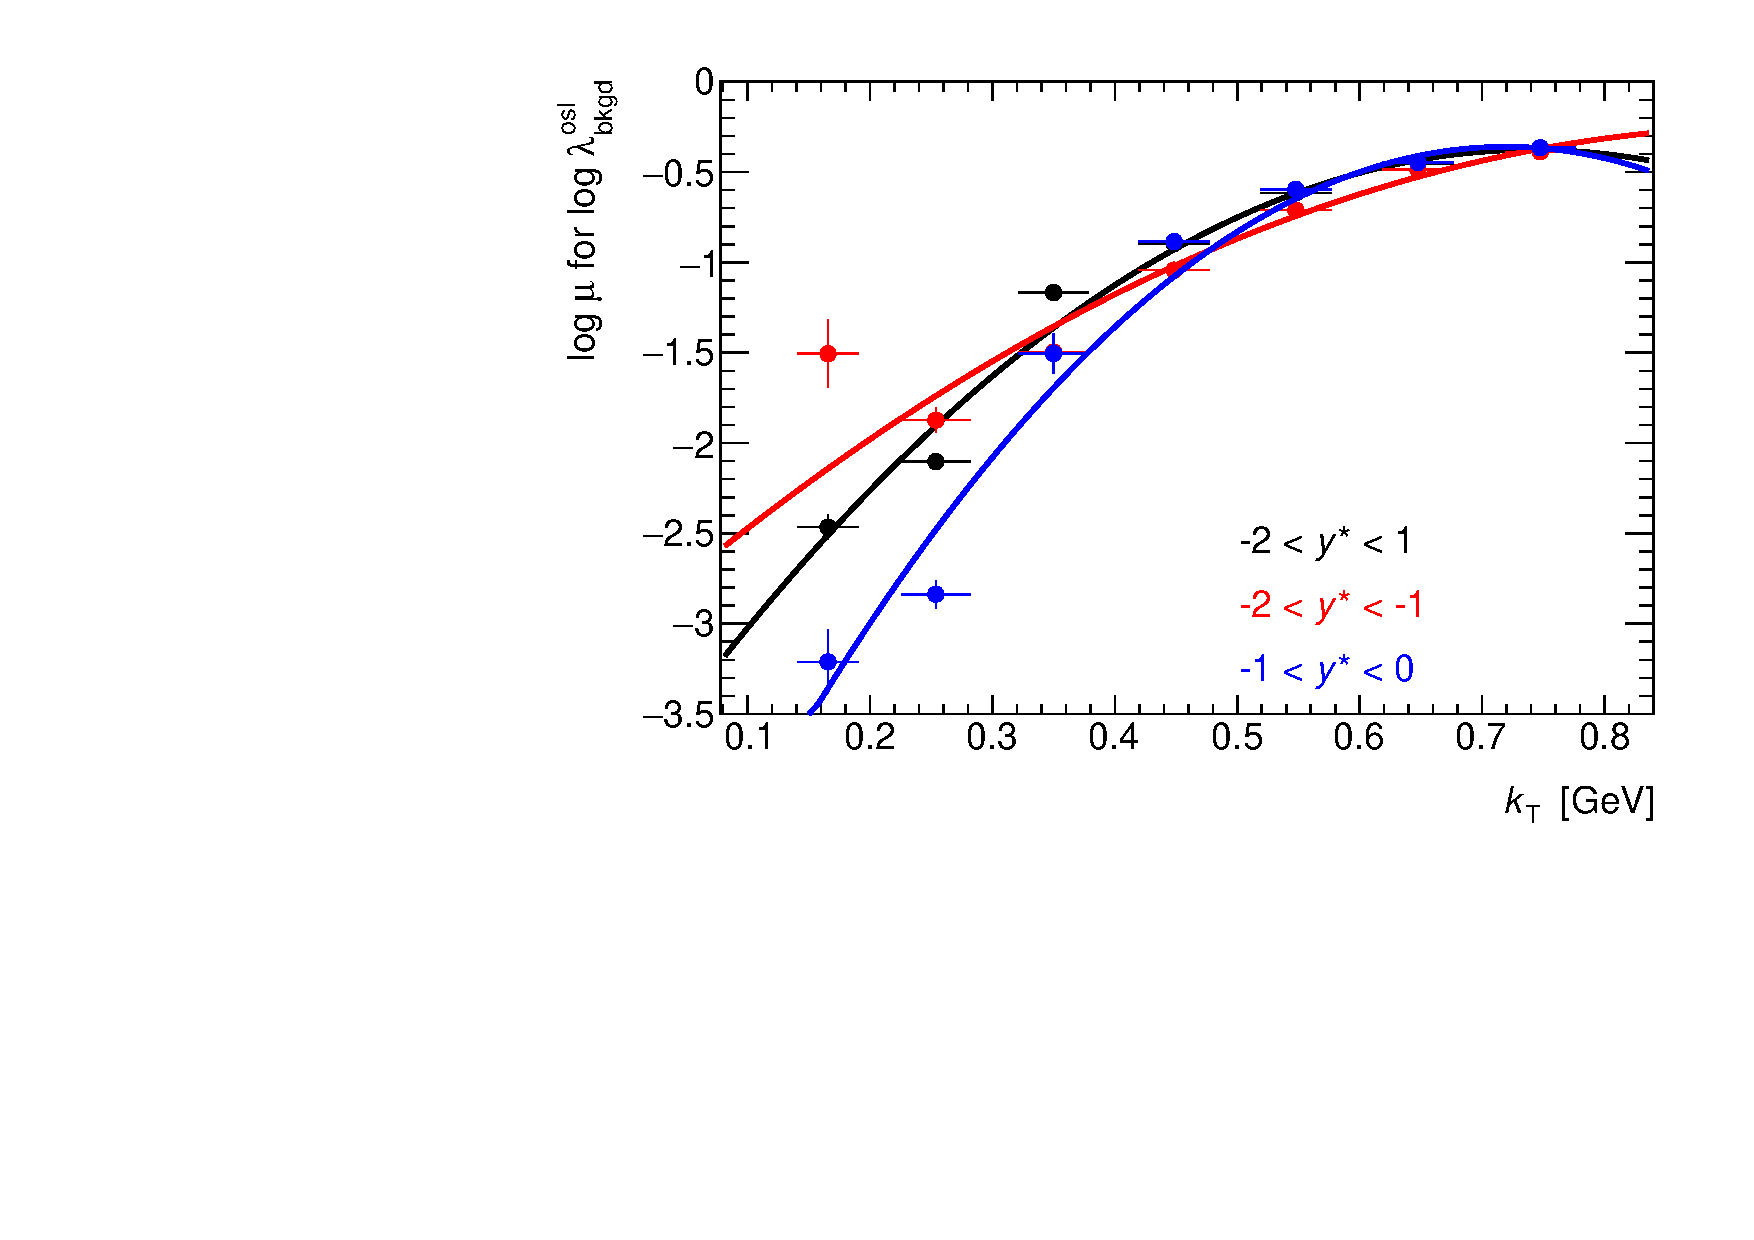
\includegraphics[width=.49\linewidth]{can_kt_qosl_backLambda_intercept_combined.pdf}
\end{minipage}
\caption{
Top: A comparison of same-sign to opposite-sign charged pairs with the amplitude and width of three-dimensional fits in \PYEight. Several multiplicities are shown in each colored \kt bin, with the multiplicity bins defined in \cref{fig:background_alpha_pythia8}, and the $++$ and $--$ pairs are separated. The slopes and intercepts of the fit lines are shown in the bottom left and right subfigures, respectively. The procedure is repeated in both forward (red) and central (blue) rapidity bins, and the difference is used as a systematic variation.}
\label{fig:background_qosl_lambda_same_vs_opp_pythia8}
\end{figure}

\begin{figure}[t]
\begin{minipage}[t]{1.0\textwidth}
\centering
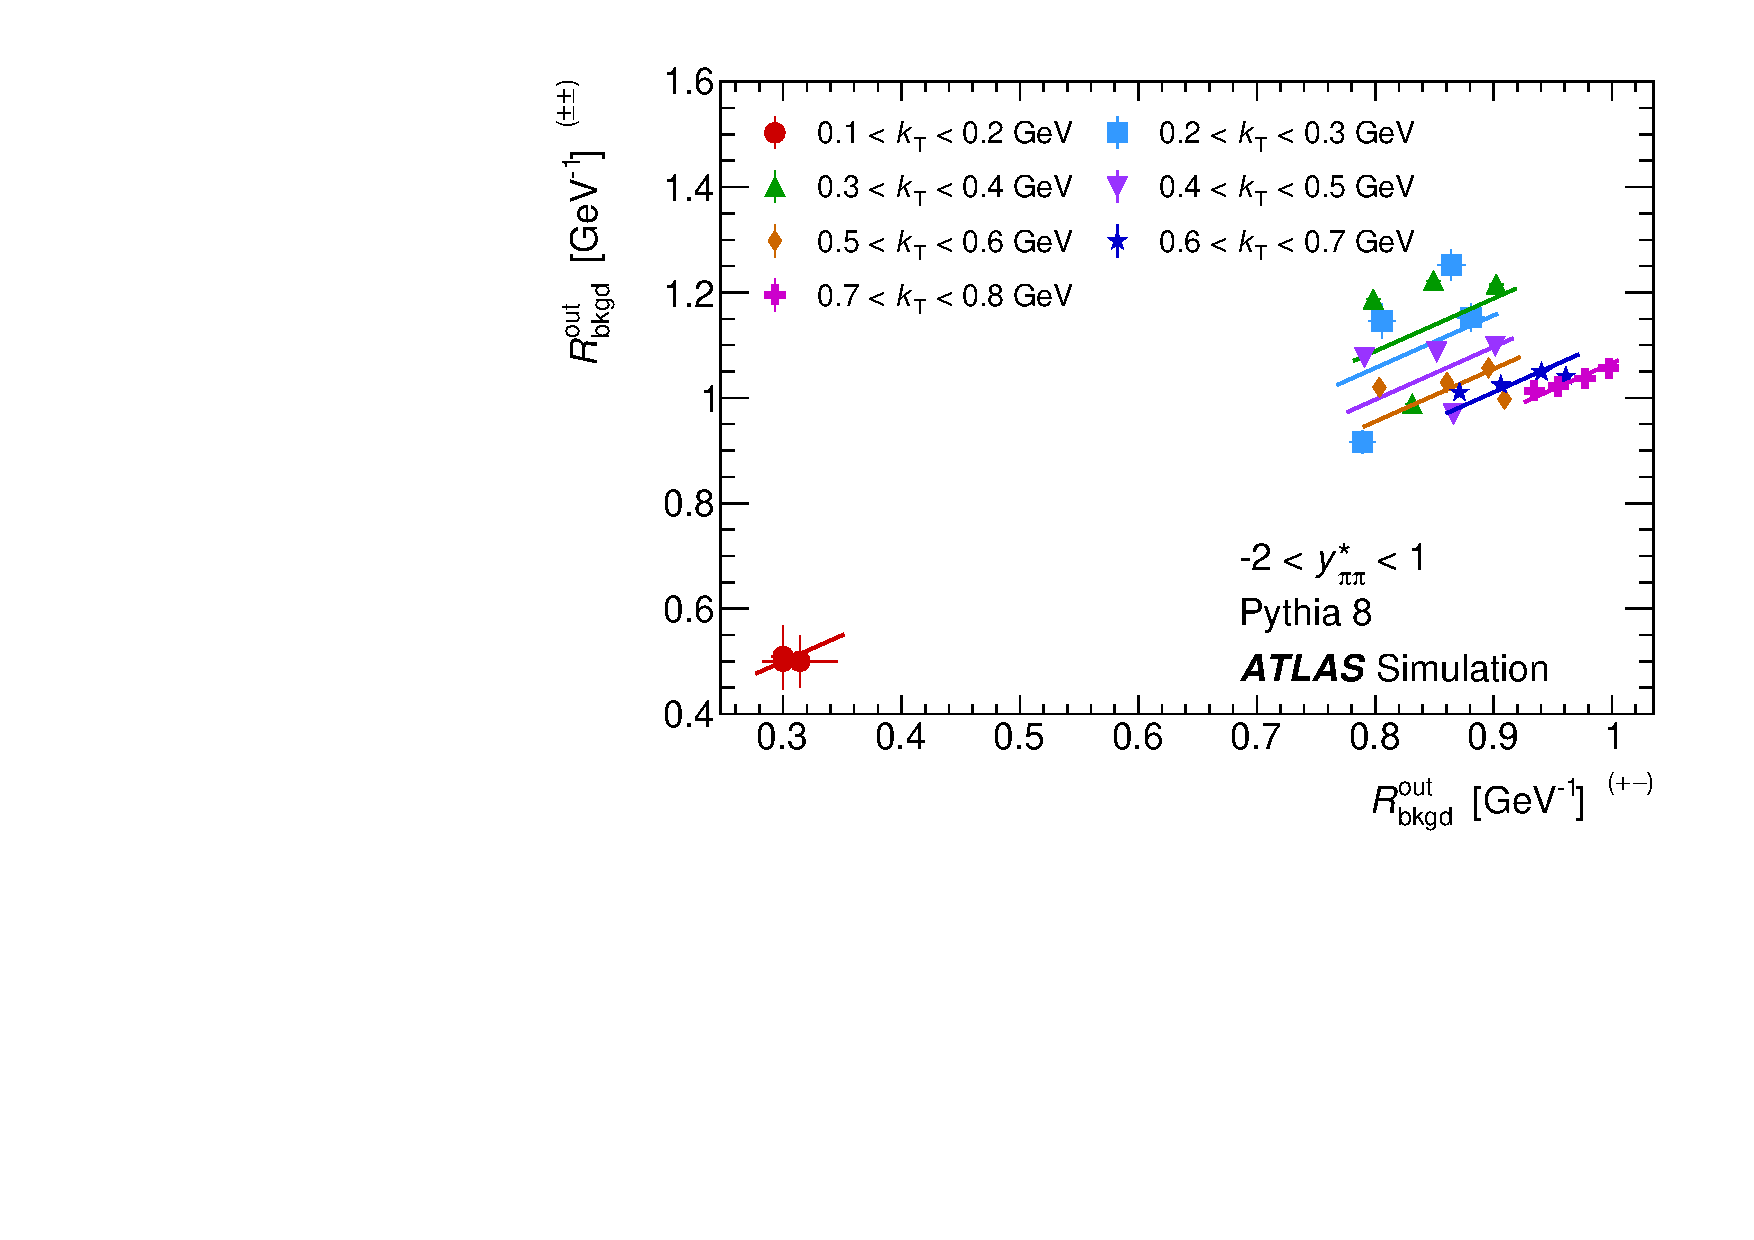
\includegraphics[width=.55\linewidth]{can_kt_qosl_backRout.pdf}
\includegraphics[width=.44\linewidth]{can_kt_qosl_backRout_intercept.pdf}
\end{minipage}
\caption{
  Left: The comparison of jet fragmentation width along the out-axis between same- and opposite- sign charged pairs. The difference is modeled as a \kt-dependent constant additive factor. Right: the best-fit difference of the width between same- and opposite-sign pairs. The lowest \kt interval is not included in the fit because the jet contribution is not large there, and its behavior does not fit the trend.
}
\label{fig:background_qosl_Rout_same_vs_opp_pythia8}
\end{figure}

\begin{figure}[t]
\begin{minipage}[t]{1.0\textwidth}
\centering
\includegraphics[width=.55\linewidth]{can_kt_qosl_backR.pdf}
\includegraphics[width=.44\linewidth]{can_kt_qosl_backR_intercept.pdf}
\end{minipage}
\caption{
  Left: The comparison of jet fragmentation width in the side-long plane between same- and opposite- sign charged pairs. The difference is modeled as a \kt-dependent constant additive factor. Right: the best-fit difference of the width between same- and opposite-sign pairs. The lowest \kt interval is not included in the fit because the jet contribution is not large there, and its behavior does not fit the trend.
}
\label{fig:background_qosl_R_same_vs_opp_pythia8}
\end{figure}


Just as is done for the \qinv correlation functions, the amplitudes for three dimensional jet correlations are compared between opposite- and same-sign pairs (\cref{fig:background_qosl_lambda_same_vs_opp_pythia8}).

\begin{align}
\lbkgd^{\mathrm{osl},\pm\pm} &= \mu(\kt) \left(\lbkgd^{\mathrm{osl}+-}\right)^{\nu(\kt)} \label{eq:lambdaBackParOSL}\\
\Rbkgd^{\mathrm{sl},\pm\pm} &= \Rbkgd^{\mathrm{sl}+-} + \Delta\Rbkgd^{\mathrm{sl}}(\kt) \label{eq:rBackParSL}\\
\Rbkgd^{\mathrm{out},\pm\pm} &= \Rbkgd^{\mathrm{out}+-} + \Delta\Rbkgd^{\mathrm{out}}(\kt) \label{eq:rBackParOut}
\end{align}

The numerical values used for mapping the amplitude $\lbkgd^\mathrm{osl}$ (\cref{fig:background_qosl_lambda_same_vs_opp_pythia8}), fragmentation width colinear with the jet axis $\Rbkgd^\mathrm{out}$ (\cref{fig:background_qosl_Rout_same_vs_opp_pythia8}), and fragmentation width transverse to the jet axis $\Rbkgd^\mathrm{sl}$ (\cref{fig:background_qosl_R_same_vs_opp_pythia8}) are as follows:

\begin{align}
\log \mu (\kt [\textrm{GeV}]) &= -3.9 + 9.5 \kt - 6.4 \kt^2 \label{eq:mu_osl}\\
\nu(\kt [\textrm{GeV}]) &= 0.03 + 2.6 \kt - 1.6 \kt^2 \label{eq:nu_osl}\\
\Delta \Rbkgd^\mathrm{out} (\kt [\textrm{GeV}]) &= 0.43 - 0.49 \kt \label{eqn_rbkgdout}\\
\Delta \Rbkgd^\mathrm{sl} (\kt [\textrm{GeV}]) &= \frac{0.51}{1 + (1.30\kt)^2} \label{eqn_rbkgdsl}
\end{align}

\FloatBarrier
\subsection{Difference between collision systems}

The mapping from opposite- to same- sign correlation functions is derived from \PYEight, which simulates \pp collisions but not nuclear collisions.
Since the background structure is caused primarily by the fragmentation of mini-jets, a large difference is not expected between \pp and \pPb systems.
Nevertheless the distinction can and should be evaluated.

\begin{figure}[t]
\includegraphics[width=.49\linewidth]{backLambda_charge_comp_ppHijing.pdf}
\includegraphics[width=.49\linewidth]{backLambda_charge_comp_pPbHijing.pdf}\\
\includegraphics[width=.49\linewidth]{qinv_backAlpha_vs_kt_ppHijing.pdf}
\includegraphics[width=.49\linewidth]{qinv_backAlpha_vs_kt_pPbHijing.pdf}\\
\caption{The background amplitude ratio (top) and the shape parameter (bottom) in \Hijing for both proton-proton (left) and proton-lead (right). The proton-lead has about a 5-20\% attenuation from proton-proton. For the amplitude comparison the width ratio from opposite to same sign is forced to be a constant 1.08, which the ratio tends to at high \kt in \Hijing for both systems. The shape, parameterized by $\abkgd$, is quite similar between the systems.}
\label{fig:background_pp_ppb_comp}
\end{figure}


\begin{figure}[t]
\includegraphics[width=\linewidth]{mu_hijing_pp_pPb.pdf}
\caption{A comparison of the attenuation between opposite- and same-sign correlation functions in \Hijing proton-proton and \Hijing proton-lead (all other settings identical). The multiplicity slices in each \kt bin are $26 \leq N_{ch}^{tr} \leq 36$, $37 \leq N_{ch}^{tr} \leq 48$, and $49 \leq N_{ch}^{tr} \leq 64$. The difference between the ratio is slightly more prominent in proton-lead, which is accounted for in the mapping and as a systematic error. The variable $\mu$ is used here because this correction and variation is applied directly into the $\mu$ of equations \cref{eq:lambdaBackPar,eq:mu}.}
\label{fig:mu_hijing_pp_pPb}
\end{figure}

Since \Hijing uses an old version of \Pythia 6 its description of the fragmentation function is not up-to-date, but \Pythia alone does not simulate the same soft particle production that \Hijing does.
Thus, \PYEight \pp is used to derive the mapping between $+-$ and $\pm\pm$, then corrected slightly for the difference between \pp and \pPb observed in \Hijing.
A comparison of \Hijing \pp and \pPb correlation functions shows that the ratio of the background width is the same in each, at least at high \kt (about 1.08).
This justifies using the width ratio from the updated \PYEight, since it suggests that changing from a proton-proton system to a proton-lead system does not drastically alter the ratio of widths.
We also see that in \Hijing (with the width ratio is fixed to 1.08) $\log \lbkgd$ is decreased in \pPb by $0.05$ (high \kt) to $0.2$ (low \kt) (See \cref{fig:background_pp_ppb_comp}). This difference is made more precise in \cref{fig:mu_hijing_pp_pPb}, which quantifies the difference in the amplitudes of the ratios of correlation functions.
The extracted scaling is applied to the background description in the data, and the spread in the attenuation is accounted for as a systematic variation.

\FloatBarrier

\subsection{Mapping results}

\begin{figure}[t]
\centering
\includegraphics[width=.49\linewidth]{Cqinv_cent0_e0_kt0_ys1.pdf}
\includegraphics[width=.49\linewidth]{Cqinv_cent4_e0_kt4_ys1.pdf}\\
\includegraphics[width=.49\linewidth]{Cqinv_cent7_e0_kt6_ys1.pdf}
\caption{Examples of the background fit to opposite-sign correlation functions in the data. The shape parameter $\abkgd$ is fixed from \PYEight, and the amplitude $\lbkgd^{+-}$ and width $\Rbkgd^{+-}$ are left as free parameters. A selection of centrality and \kt bins are chosen to cover a large range of the magnitude of the effect. Some resonances are removed before filling the histograms, which accounts for the gaps and large error bars in some bins.}
\label{fig:background_qinv_opp_example}
\end{figure}

\Cref{fig:background_qinv_opp_example} shows a few examples of the fit to opposite-sign correlation functions in order to determine the background.
These fit parameters are then used with the mapping derived from the Monte Carlo to fix the background in same-sign fits.
The parameters used to describe the background in \qinv are shown in \cref{fig:background_data}.

\begin{figure}[t]
\begin{minipage}[t]{1.0\textwidth}
\centering
\includegraphics[width=.49\linewidth]{canqinv_backLambda_vs_kt_opp.pdf}
\includegraphics[width=.49\linewidth]{canqinv_backLambda_vs_kt_same.pdf}\\
\includegraphics[width=.49\linewidth]{canqinv_backR_vs_kt_opp.pdf}
\includegraphics[width=.49\linewidth]{canqinv_backR_vs_kt_same.pdf}\\
\end{minipage}
\caption{The background parameters that are free fit parameters in the opposite sign (left), and the like-sign parameters derived from the opposite-sign values using \cref{eq:lambdaBackPar,eq:rBackPar,eq:mu,eq:nu} (right). The $\abkgd$ parameter is taken directly from \PYEight (\cref{fig:background_alpha_pythia8}). Statistical error bars are too small to be visible. The non-monotonicity is not surprising, since the meaning of $\Rbkgd$ changes with $\abkgd$, which varies with \kt as shown in \cref{fig:background_alpha_pythia8,fig:background_pp_ppb_comp}.}
\label{fig:background_data}
\end{figure}


%---------------------------------------------
\subsection{Fits to \Pythia}
\label{subsec:pythia_fits}
%---------------------------------------------

This section will show examples of how well the stretched exponential form fits the correlation functions in \PYEight.
The parameters extracted from these fits are used to form the mapping from opposite sign to same sign in the background description of the data.
A moderate multiplicity bin is shown in \cref{fig:pythia_bkgd_fit_cent3}.

\begin{figure}[t]
\includegraphics[width=.49\linewidth]{Cqinv_pythia_cent3_e0_kt0.pdf}
\includegraphics[width=.49\linewidth]{Cqinv_pythia_cent3_e1_kt0.pdf}\\
\includegraphics[width=.49\linewidth]{Cqinv_pythia_cent3_e0_kt3.pdf}
\includegraphics[width=.49\linewidth]{Cqinv_pythia_cent3_e1_kt3.pdf}\\
\includegraphics[width=.49\linewidth]{Cqinv_pythia_cent3_e0_kt6.pdf}
\includegraphics[width=.49\linewidth]{Cqinv_pythia_cent3_e1_kt6.pdf}\\
\caption{Fits of the stretched exponential to correlation functions from \PYEight events with a truth-level multiplicity in the range of $49 \leq \Nch \leq 64$.}
\label{fig:pythia_bkgd_fit_cent3}
\end{figure}

%% skip low mult
% \begin{figure}[t]
% \includegraphics[width=.49\linewidth]{Cqinv_pythia_cent7_e0_kt0.pdf}
% \includegraphics[width=.49\linewidth]{Cqinv_pythia_cent7_e1_kt0.pdf}\\
% \includegraphics[width=.49\linewidth]{Cqinv_pythia_cent7_e0_kt3.pdf}
% \includegraphics[width=.49\linewidth]{Cqinv_pythia_cent7_e1_kt3.pdf}\\
% \includegraphics[width=.49\linewidth]{Cqinv_pythia_cent7_e0_kt6.pdf}
% \includegraphics[width=.49\linewidth]{Cqinv_pythia_cent7_e1_kt6.pdf}\\
% \caption{Fits of the stretched exponential to correlation functions from \PYEight events.}
% \label{fig:pythia_bkgd_fit_cent7}
% \end{figure}


\FloatBarrier
%---------------------------------------------
\subsection{Comparison of \Herwig and \PYEight}
\label{subsec:herwig_vs_pythia}
%---------------------------------------------

Both \PYEight and \Herwig++ are studied in order to understand the uncertainties inherent in the background description.
A direct comparison of the two is shown in \cref{fig:comp_herwig_pythia_cent3}.
\Herwig tends to overestimate the mini-jet background more prominently than \PYEight does, especially at low \kt.
\Cref{fig:herwig_pythia8_cent3_bkgd_charge_comp} compares the same and opposite sign correlation functions in the simulations considered.

\begin{figure}[t]
% \includegraphics[width=.49\linewidth]{herwigPythiaCompCent3_e0_kt0.pdf}
% \includegraphics[width=.49\linewidth]{herwigPythiaCompCent3_e1_kt0.pdf}
\includegraphics{herwigPythiaCompCent3_e0_kt3.pdf}
\includegraphics{herwigPythiaCompCent3_e1_kt3.pdf}
% \includegraphics[width=.49\linewidth]{herwigPythiaCompCent3_e0_kt6.pdf}
% \includegraphics[width=.49\linewidth]{herwigPythiaCompCent3_e1_kt6.pdf}
\caption{An illustration of the differences between the jet fragmentation contribution to $C(\qinv)$ predicted in \Herwig and \PYEight, for relatively higher multiplicities $49 \leq N_\mathrm{ch}^\mathrm{tr} \leq 64$. The ratio of \Herwig to \PYEight is shown in the lower boxes of each plot. Opposite- (same-)charge correlation functions are shown on the left (right).}%, and from top to bottom the figures have increasing \kt.}
\label{fig:comp_herwig_pythia_cent3}
\end{figure}

% \begin{figure}[t]
% \includegraphics[width=.49\linewidth]{herwigPythiaCompCent7_e0_kt0.pdf}
% \includegraphics[width=.49\linewidth]{herwigPythiaCompCent7_e1_kt0.pdf}
% \includegraphics[width=.49\linewidth]{herwigPythiaCompCent7_e0_kt3.pdf}
% \includegraphics[width=.49\linewidth]{herwigPythiaCompCent7_e1_kt3.pdf}
% \includegraphics[width=.49\linewidth]{herwigPythiaCompCent7_e0_kt6.pdf}
% \includegraphics[width=.49\linewidth]{herwigPythiaCompCent7_e1_kt6.pdf}
% \caption{An illustration of the differences between the jet fragmentation contribution to $C(\qinv)$ predicted in \Herwig and \PYEight, for relatively lower multiplicities $26 \leq N_\mathrm{ch}^\mathrm{tr} \leq 36$. The ratio of \Herwig to \Pythia is shown in the lower boxes of each plot. Opposite- (same-)sign correlation functions are shown on the left (right), and from top to bottom the figures have increasing \kt.}
% \label{fig:comp_herwig_pythia_cent7}
% \end{figure}

\begin{figure}[t]
% \includegraphics[width=.49\linewidth]{herwig_bkgd_charge_comp_cent3_kt0.pdf}
% \includegraphics[width=.49\linewidth]{pythia8_bkgd_charge_comp_cent3_kt0.pdf}\\
% \includegraphics[width=.49\linewidth]{herwig_bkgd_charge_comp_cent3_kt2.pdf}
% \includegraphics[width=.49\linewidth]{pythia8_bkgd_charge_comp_cent3_kt2.pdf}\\
\includegraphics{herwig_bkgd_charge_comp_cent3_kt4.pdf}
\includegraphics{pythia8_bkgd_charge_comp_cent3_kt4.pdf}\\
% \includegraphics[width=.49\linewidth]{herwig_bkgd_charge_comp_cent3_kt6.pdf}
% \includegraphics[width=.49\linewidth]{pythia8_bkgd_charge_comp_cent3_kt6.pdf}\\
\caption{A comparison of like and unlike sign correlation functions in \Herwig++ and \PYEight.}
\label{fig:herwig_pythia8_cent3_bkgd_charge_comp}
\end{figure}

% \begin{figure}[t]
% \includegraphics[width=.49\linewidth]{herwig_bkgd_charge_comp_cent7_kt0.pdf}
% \includegraphics[width=.49\linewidth]{pythia8_bkgd_charge_comp_cent7_kt0.pdf}\\
% \includegraphics[width=.49\linewidth]{herwig_bkgd_charge_comp_cent7_kt2.pdf}
% \includegraphics[width=.49\linewidth]{pythia8_bkgd_charge_comp_cent7_kt2.pdf}\\
% \includegraphics[width=.49\linewidth]{herwig_bkgd_charge_comp_cent7_kt4.pdf}
% \includegraphics[width=.49\linewidth]{pythia8_bkgd_charge_comp_cent7_kt4.pdf}\\
% \includegraphics[width=.49\linewidth]{herwig_bkgd_charge_comp_cent7_kt6.pdf}
% \includegraphics[width=.49\linewidth]{pythia8_bkgd_charge_comp_cent7_kt6.pdf}\\
% \caption{A comparison of like and unlike sign correlation functions in \PYEight.}
% \label{fig:herwig_pythia8_cent7_bkgd_charge_comp}
% \end{figure}

\begin{figure}[t]
\begin{minipage}[t]{\textwidth}
\centering
\includegraphics[width=\linewidth]{mu_pythia_herwig.pdf}
\end{minipage}
\caption{The left plot compares the difference in $+-$ and $\pm\pm$ correlation function ratios between two generators. The multiplicity bins used are $26 \leq N_{ch}^{tr} \leq 36$, $37 \leq N_{ch}^{tr} \leq 48$, and $49 \leq N_{ch}^{tr} \leq 64$. The lowest \kt bin is not used because of large statistical fluctuations in the fit parameters. While \Herwig predicts an amplitude for the ratio $C^{+-}/C^{\pm\pm}$ that is clearly too small by inspection (i.e. it blatantly fails to match the correlation functions in the data), the variation of the double ratio (\Herwig to \PYEight) can be used to showcase the uncertainty in a constant attenuation factor.}
\label{fig:delta_mu_pythia_herwig}
\end{figure}

\subsection{Incorporating the hard-process description into fit}

This section will briefly summarize the process by which the jet background is measured and applied in the data analysis.
An example using the Lorentz-invariant correlation functions is shown in \cref{fig:hp_example}.

\begin{figure}[t]
\centering
\includegraphics{cqinv_charge_comp_cent6_kt4_kys1.pdf}
\caption{Correlation functions in proton-lead data for opposite-charge (teal circles) and same-charge (red squares) pairs. The opposite-charge correlation function, with the most prominent resonances removed, is fit to a function of the form in \cref{eq:jet_frag_form_inv} (blue dashed line). The violet dotted line is the estimated jet contribution in the same-charge correlation function, also of the form of \cref{eq:jet_frag_form_inv}, and the dark red line is the full fit of \cref{eq:correlation_function_full} to the same-charge data.}
\label{fig:hp_example}
\end{figure}

With $\abkgdinv(\kt)$, $\mu(\kt)$, $\nu(\kt)$, and $\rho$ determined from Monte Carlo generator samples, the mapping can be applied to the \pPb data.
As illustrated in \cref{fig:hp_example}, the $+-$ correlation function is fit to \cref{eq:jet_frag_form_inv} for $\qinv > 0.1~\GeV$, with \abkgd fixed from \PYEight and $\lbkgdinv{}^{+-}$ and $\Rbkgdinv{}^{+-}$ as free parameters.
The $\mu$, $\nu$, and $\rho$ parameters are used to infer $\lbkgdinv{}^{\pm\pm}$ and $\Rbkgdinv{}^{\pm\pm}$, which are fixed before the femtoscopic part of the correlation function is fit to $\pm\pm$ data.

\FloatBarrier


%% -------------------------------------------
%% Systematics
%% -------------------------------------------
\section{Systematic uncertainties and cross-checks}
\label{sec:systematics}

The average effect of each systematic on \Rinv is shown in \cref{table:rinv_syst} for each \kt bin.
The systematics in two centrality bins are shown in \cref{table:rinv_syst_central,table:rinv_syst_peripheral}.
Similar tables are shown for the 3D radii in \cref{table:rout_syst,table:rside_syst,table:rlong_syst}.
The systematics listed there are included in the final results.

\subsection{Generator for hard-process description}
The greatest difficulty by far in measuring \ac{HBT} radii in small systems is in forming an accurate description of the background contribution from hard processes.
For the uncertainty in the hard-process contribution two effects are considered.
First, the variation in the translation from \pp to \pPb is taken as an uncertainty in the amplitude, as shown in \cref{fig:mu_hijing_pp_pPb}.
Secondly, as described in \cref{subsec:herwig_vs_pythia}, the width of the variation in the difference of $\frac{C^{+-}}{C^{\pm\pm}}$ between \Pythia and \Herwig (\cref{fig:delta_mu_pythia_herwig}) is used as an additional systematic variation in the background amplitude.
This is to account for uncertainty arising from the specific choice of \Pythia as a generator.
Both uncertainties are expressed as a scaling factor times $\lbkgd$, so they can be evaluated by scaling $\mu$ (\cref{eq:lambdaBackPar,eq:mu}):

\begin{equation}
\sigma_{\log \mu} = \sigma^{pp \rightarrow p+\mbox{Pb}1}_{\log \mu} \oplus \sigma^{\Pythia-\textrm{\Herwig}}_{\log \mu} = 0.0413 \oplus 0.116 = 0.123
\end{equation}

The background amplitude \lbkgd is thus scaled up and down by 12.3\% to compute the systematic from the background.

\subsection{Rapidity dependence of hard-process description}

The background amplitude relations in \cref{eq:lambdaBackPar,eq:rBackPar} are evaluated with \Pythia in both central ($|\kys| < 1$) and forward ($1 < |\kys| < 2$) rapidity intervals.
The width relationship (\cref{eq:rBackPar}) does not change significantly, but the relationship between the amplitudes (\cref{eq:lambdaBackPar}) does.
The parameterization is varied from the nominal (inclusive) expression to that for each of the different rapidity bins.
In three dimensions a 2nd-order polynomial is used instead of a sigmoid.
This variation is illustrated in \cref{subsec:jet_frag_inv,subsec:jet_frag_3d}.

\subsection{Jet fragmentation background in 3D}

One alternative to \cref{eq:jet_frag_form_3d} is to describe the jet fragmentation in three dimensions as a simple function of \qinv only.
The average \kt in each centrality/\kt/\kys interval can be used in \cref{eq:q3_to_qinv} to contract $\mathbf{q}$ into \qinv.
The same parameters derived in the Lorentz invariant correlations could be used to describe the three-dimensional background as well.
This turns out to be an over-simplification, as shown in \cref{fig:pythia_qosl_alt_bkgd}.
The form in \cref{eq:jet_frag_form_3d} is used as it clearly describes the jet fragmentation more accurately.

\begin{figure}[t]
\begin{minipage}[t]{\textwidth}
\centering
\includegraphics[width=\linewidth]{can_Cqosl_pythia_altbkgd_cent7_e3_kt6_ys1.pdf}
\end{minipage}
\caption{Two functional forms for describing three-dimensional jet fragmentation. The blue line (\cref{eq:jet_frag_form_3d}) is the one used in the results, and the purple line (which describes the correlation as a function of \qinv only) clearly does not enjoy the same level of agreement.}
\label{fig:pythia_qosl_alt_bkgd}
\end{figure}


\subsection{Shape parameters of hard-process description}
The background parameters $\abkgd^\mathrm{inv}$, $\abkgd^\mathrm{out}$, and $\abkgd^\mathrm{sl}$ were varied by 0.1\% from the nominal values.
The typical effect on the \ac{HBT} radii was seen to be on order 0.5\%, and this variation is not included in the reported systematic errors.

\subsection{Pion identification}
The \ac{PID} definition used for the nominal result is the ``Middle'' cut level defined in \cref{sec:pid}.
Systematic uncertainties from imperfections in the particle identification are evaluated by repeating the analysis with both the ``Loose'' and ``Tight'' cut levels.
The effect on the radii is around 1--2\% for the lower \kt bins, but becomes more significant at higher momentum bins (presumably because they are relatively more populated with kaons and protons).

\subsection{Charge asymmetry}
The distinction between positive and negative pairs could come from the orientation of the overlap of the inner detector components.
The nominal value is taken to be the fit results from histograms filled with all same-sign pairs, and a systematic variation is taken to positive and negative pairs.

\subsection{Binning of $z$ position of Primary Vertex}
A significant difference in the radii at high \kt was observed when it was required that events only be mixed from within the same 5 mm wide bin in $z_\textrm{vtx}$, the longitudinal position of the primary vertex.

The variations in the radii between a bin size of 2 mm and 5 mm were found to be around $0.5 \%$, so a bin size of 5 mm is chosen and a systematic uncertainty is neglected.
It is required that the event-mixing buffer in a given $z_\textrm{vtx}$ bin be full before histograms are filled, which ensures that the signal and mixed-event background have the same $z_\textrm{vtx}$ distribution.

\subsection{Core fraction $x_c$}
A correlation function of the form

\begin{equation}
C(q) = \left[1-x_c + x_c K(\qinv)\left( 1 + \lambda e^{-Rq} \right) \right] \Omega(q)
\end{equation}

was also considered.
In this form $\lambda$ takes into account pion impurities, and $x_c$ indicates the fraction of pairs that come from a core (i.e. not from long-lived resonances or weak decays - see \cref{fig:pythia_xc}).
The region of the correlation function that drives the fit results is both at a larger $\qinv$ than where the Coulomb correction $K(\qinv) \neq 1$ and at smaller $\qinv$ than where $e^{-\Rinv\qinv}$ can be neglected.
Here the correlation function looks like $C(q) \approx 1 + x_c \lambda e^{-Rq} \Omega(q)$, so the results are mostly dependent only on the product $x_c \lambda$.

The measured radii turn out to be for the most part extremely insensitive to variations in the core fraction $x_c$.
To emphasize this, $x_c$ is varied between 0.4 and 0.9.
This is surely an overestimation of the possible range, but the difference in the radii is still less than one percent for nearly all bins.

\begin{figure}[t]
\begin{minipage}[t]{1.0\textwidth}
\centering
\includegraphics{pythia_xc.pdf}
\end{minipage}
\caption{The core fraction $x_c$ measured in \PYEight by counting the pairs in which neither particle is a product of a weak decay or of a $\eta$, $\eta'$, $\omega$, or $K*$.}
\label{fig:pythia_xc}
\end{figure}

Though a core fraction near 50\% is physically reasonable (as in \cref{fig:pythia_xc}), it results in $\lambda$ parameters near 2.
$\lambda$ should always be less than 1 in order to be interpreted as a coefficient of a Bose-Einstein enhancement.
There is a redundancy in the description of the correlation function using both $x_c$ and $\lambda$.

To avoid over-parameterizing the fit and to avoid questionable values of $\lambda$, the choice was made to take $\lambda = 1$ and rename $x_c \rightarrow \lambda$, to match the form of the Bowler-Sinyukov formula \[C(q) = \left[ 1-\lambda + \lambda K(\qinv)\left( 1 + e^{-Rq} \right)\right] \Omega(q) \;.\]

\subsection{Effective size for the Coulomb effect}
The non-zero effective size of the Coulomb correction \Reff should only provide a bin-by-bin difference of a few percent, even up to several fm.
However, because the parameter effectively changes the $\mathbf{q}$ range over which the Coulomb correction is applied, varying this parameter can affect the \ac{HBT} radii significantly.
The parameter \Reff is taken to be proportional to the invariant \ac{HBT} radius, such that $\Reff = \xi \Rinv$.

The nominal value of $\xi$ is chosen to be equal to unity, and a variation down to $1/2$ and up to $2$ is taken to be the $1\sigma_{syst}$ level.

\subsection{Projection of $\mathbf{q}$ onto $\qinv$}
The value of \kt used to calculate \qinv from $\mathbf{q}$ in the 3D fits (see \cref{eq:q3_to_qinv}) is varied $\pm 1$ standard deviation of the \kt in each bin.
In three dimensions, the value of \qinv is only used in the Coulomb correction.
The effect on the radii is small, and the Coulomb correction is already varied through \Reff, so this variation is not included.
%%It is still included as a systematic in the 3D results.

%%is not expected to change \Rside or \Rlong appreciably since the part of the correlation function most relevant to those parameters is at $\qout = 0$, where $\qinv = |\mathbf{q}|$. It could possibly have a measureable effect on \Rout, however.

\subsection{Alternative test statistic}

As an alternative check to the previous method, a Poisson log-likelihood that accounts for uncertainty in both the signal and background can also be used.
The mixed-event background is weighted by the Coulomb factor $K(\qinv)$ from the discussion in \cref{subsec:coulomb}.
\begin{equation}
  \tilde{B} \equiv (1-\lambda)B + \lambda B_{K} C_{\textrm{BE}}
\end{equation}
$B_{K}$ denotes the background formed by weighting each pair by the Coulomb correction $K(\qinv)$.
The variance in a given bin is
\begin{equation}
  \sigma_{\tilde{B}}^2 = (1-\lambda)^2 B + 2\lambda(1-\lambda)B_{K} C_{\textrm{BE}} + \lambda^2 B_{K^2} C_{\textrm{BE}}^2
\end{equation}
where following the notation introduced above, $B_{K^2}$ is the mixed-event background in which each pair is weighted by the square of $K(\qinv)$.
The negative log-likelihood ratio that is minimized is then \cite{Soltz:1994PhDT} % Zajc's method
\begin{equation}
  - 2\ln \mathcal{L} = -2 \sum_{q_i} \left[ A - \tilde{B} + \left( A + \sigma_{\tilde{B}}^2 \right) \ln \left(1 - \frac{A - \tilde{B}}{A + \sigma_{\tilde{B}}^2} \right) \right]
\end{equation}
The alternative test statistic mentioned is checked to to ensure that the fit results do not vary significantly as a result and the typical variation is less than $0.1\%$, well within the statistical uncertainties.


\subsection{Two-particle track reconstruction effects}
It is typically assumed that effects like tracking efficiency and acceptance factor out of the ratio $A(q) / B(q)$.
However, one can reasonably question whether two-particle effects like ghosting can affect the correlation function.
To explore this possibility, the ratio of reconstructed to truth correlation functions are shown in \cref{fig:2pc_effects}.
A significant effect above the few lowest \qinv bins is not observed.

\begin{figure}[t]
\begin{minipage}[t]{1.0\textwidth}
\centering
\includegraphics[width=.49\linewidth]{Cqinv_hijing_reco_vs_truth_cent3_e3_kt1.pdf}
\includegraphics[width=.49\linewidth]{Cqinv_hijing_reco_vs_truth_cent3_e3_kt6.pdf}
\end{minipage}
\caption{A comparison of reconstructed to truth correlation functions using reconstructed \Hijing events.
The bottom shows the ratio of truth to reconstructed correlation functions.}
\label{fig:2pc_effects}
\end{figure}

A minimum $q$ cutoff is applied in the fits to avoid being affected by detector effects like resolution and ghosting.
The sensitivity of the results to this limit is checked by taking $\qinv^\textrm{min} = 30 \pm 10 \MeV$ in the 1D fits and symmetrizing the effect of the variation from $|\mathbf{q}|^\textrm{min} = 25 + 25 \MeV$ in the 3D fits.

\subsection{Difference between two runs}

A useful cross-check on the measurement is that the results should not differ significantly between period A (Pb going in $+z$ direction) and period B (proton going in $+z$ direction).
\cref{fig:fit_inv_R_split} illustrates the difference observed between the two runs, which is not significant.
The differences are comparable to statistical uncertainties - typically less than $0.5\%$ at low \kt and around $2\%$ at the upper end of the \kt bins.

\begin{figure}[t]
\includegraphics[width=.49\linewidth]{qinv_R_vs_kt_periodA.pdf}
\includegraphics[width=.49\linewidth]{qinv_R_vs_kt_periodB.pdf}
\caption{Results for \Rinv split into both periods and both signs as a check.
No systematic uncertainties are included - this is intended as a cross-check.}
\label{fig:fit_inv_R_split}
\end{figure}

\FloatBarrier %% split azimuthal plots

\subsection{Event plane resolution}
Uncertainty in the 2nd-order event plane resolution is propagated through the event plane resolution correction to the azimuthally-dependent results. There are two contributions to the \psit resolution, both of which are evaluated by changes to the two alternate sub-detectors used in the three-sub-detector method of evaluating $\langle \cos(2\delta\psit) \rangle$. For one variation, tracks weighted by their \pt are used instead of calorimeter cells, and for the other the rapidity windows of the alternate subsdetectors are shifted away from the nominal sub-detector by $\Delta\eta = 0.5$.

\subsection{Sampling uncertainty}
The effect of the sampling procedure on the pair distribution is evaluated by taking the ratio of the distributions of sampled pairs to traditional event-mixed pairs, as discussed in \cref{subsec:bkgd_sampling}.
The uncertainty is determined by evaluating this ratio in the 8 intervals of $\kphi - \psit$ and 5 intervals of flow $|\qt|$, and using one standard deviation at the endpoints of the middle 68.27\% interval (\cref{fig:sample_to_mix_ratio}).
%% The uncertainty is determined by evaluating this ratio in each event class and in several intervals of $\kphi - \psit$ and using the endpoints of the middle 68.27\% interval of this whole collection (\cref{fig:sample_to_mix_ratio_kt2}).
This procedure is measured separately for each \kt bin.

\subsection{Azimuthal de-correlation in rotated event mixing}
The sampling procedure necessitates an effective integration over event plane angle \psit, or the computing demands of the analysis would be unmanageable. While there is no dependence of the physics on the event plane angle due to average rotational symmetry of the collisions, variations in the track reconstruction efficiency can affect the correlation between pairs of tracks. A pair distribution formed with event mixing is compared to a similar distribution in which one event is rotated azimuthally by a uniform random angle. The ratio of these distributions indicates the effect of the detector response on the pair correlation. The pair distribution is corrected by this ratio. The uncertainty in the ratio is evaluated by taking the endpoints of the middle 68.27\% of the variation in different runs and multiplicity bins (\cref{fig:phi_corr_to_uncorr_ratio}). This accounts for variations in the pair response that may change between runs.

\FloatBarrier
\subsection{Summary tables and plots}
Examples of the systematic uncertainties in the invariant parameters \Rinv and \linv are shown as a function of \kt and centrality in \cref{fig:syst_rinv,fig:syst_linv}.
Typical systematic uncertainties are also shown for the 3D radii \Rout (\cref{fig:syst_rout}), \Rside (\cref{fig:syst_rside}), \Rlong (\cref{fig:syst_rlong}), and \Rol (\cref{fig:syst_rol}), as well as the ratio $\Rout / \Rside$ (\cref{fig:syst_rout_over_rside}) and the amplitude (\cref{fig:syst_losl}).

\begin{center}
\begin{table}
\begin{tabular}{r || c | c | c | c | c | c | c |}
  \hline
  \kt [GeV] & 0.1-0.2 & 0.2-0.3 & 0.3-0.4 & 0.4-0.5 & 0.5-0.6 & 0.6-0.7 & 0.7-0.8 \\
  \hline \hline
  \lbkgd & 2.1\% & 3.1\% & 5.5\% & 7.9\% & 10\% & 14\% & 19\% \\
  \hline
  Rapidity dependence of \lbkgd & 3.6\% & 4.1\% & 5.1\% & 6.6\% & 2.1\% & 1.2\% & 1.1\% \\
  \hline
  Effective Coulomb size  & 1.3\% & 1.1\% & 1\% & 0.95\% & 0.92\% & 0.9\% & 0.9\% \\
  \hline
  Pion identification & 1.3\% & 2.2\% & 2.8\% & 3.3\% & 3.8\% & 4.3\% & 4.8\% \\
  \hline
  Charge asymmetry  & 0.42\% & 0.47\% & 0.71\% & 0.58\% & 0.79\% & 1.3\% & 1.6\% \\
  \hline
  Minimum $q$ in fit  & 0.77\% & 1\% & 1.3\% & 1.2\% & 1.2\% & 0.91\% & 0.88\% \\
  \hline \hline 
  All & 4.7\% & 6\% & 8.6\% & 11\% & 12\% & 15\% & 20\% \\
  \hline
\end{tabular}
\caption{The effect of each systematic on \Rinv, averaged over centrality and rapidity. The quadrature average of the upper and lower systematic errors are divided by the value, which is averaged equally over centrality bins from 0\% to 80\%. The total is the same quantity evaluated when all systematic variations are used, so its square is not necessarily equal to the sum of squares of all the individual contributions (though it should not be drastically different).}
\label{table:rinv_syst}
\end{table}

\begin{table}
\begin{tabular}{r || c | c | c | c | c | c | c |}
  \hline
  \kt [GeV] & 0.1-0.2 & 0.2-0.3 & 0.3-0.4 & 0.4-0.5 & 0.5-0.6 & 0.6-0.7 & 0.7-0.8 \\
  \hline \hline
  \lbkgd & 1.4\% & 2.1\% & 3.5\% & 4.8\% & 6.9\% & 10\% & 14\% \\
  \hline
  Rapidity dependence of \lbkgd  & 2.8\% & 3.1\% & 1.3\% & 3.5\% & 1.8\% & 0.56\% & 0.33\% \\
  \hline
  Effective Coulomb size  & 1.2\% & 1.1\% & 1.1\% & 1\% & 1.1\% & 1\% & 1\% \\
  \hline
  Pion identification  & 0.2\% & 0.58\% & 0.52\% & 1.4\% & 2.8\% & 4.6\% & 4.9\% \\
  \hline
  Charge asymmetry  & 1.2\% & 0.14\% & 0.44\% & 1.7\% & 1.4\% & 5.9\% & 1.6\% \\
  \hline
  Minimum $q$ in fit  & 0.48\% & 0.66\% & 0.75\% & 0.6\% & 1\% & 0.34\% & 0.77\% \\
  \hline \hline 
  All  & 3.6\% & 4\% & 4\% & 6.5\% & 7.9\% & 13\% & 15\% \\
  \hline
\end{tabular}
\caption{The relative systematic uncertainties in \Rinv in the 1-5\% centrality interval. The quadrature average of the upper and lower systematic errors are divided by the nominal value to compute the relative uncertainty. The uncertainty is dominated by the hard-process background description and the contribution from the effective Coulomb size \Reff is also significant at low \kt.}
\label{table:rinv_syst_central}
\end{table}

\begin{table}
\begin{tabular}{r || c | c | c | c | c | c | c |}
  \hline
  \kt [GeV] & 0.1-0.2 & 0.2-0.3 & 0.3-0.4 & 0.4-0.5 & 0.5-0.6 & 0.6-0.7 & 0.7-0.8 \\
  \hline \hline
  \lbkgd & 2.1\% & 3.3\% & 6.2\% & 8.5\% & 11\% & 15\% & 20\% \\
  \hline
  Rapidity dependence of \lbkgd  & 4.6\% & 5.9\% & 8.4\% & 7.5\% & 2\% & 1.7\% & 1.7\% \\
  \hline
  Effective Coulomb size & 1.3\% & 1.2\% & 0.97\% & 0.87\% & 0.83\% & 0.81\% & 0.78\% \\
  \hline
  Pion identification  & 2.4\% & 4\% & 4.3\% & 4.2\% & 5.1\% & 7.7\% & 11\% \\
  \hline
  Charge asymmetry  & 0.96\% & 0.66\% & 0.33\% & 3.5\% & 0.14\% & 1.5\% & 1.4\% \\
  \hline
  Minimum $q$ in fit & 0.9\% & 0.67\% & 1.5\% & 1.4\% & 0.94\% & 0.38\% & 1.2\% \\
  \hline \hline 
  All  & 5.9\% & 8\% & 11\% & 13\% & 13\% & 17\% & 23\% \\
  \hline
\end{tabular}
\caption{The relative systematic uncertainties in \Rinv for the 60-70\% centrality interval, as in Table \ref{table:rinv_syst_central}. The uncertainty is dominated by the hard-process background description.}
\label{table:rinv_syst_peripheral}
\end{table}

\begin{table}
\begin{tabular}{r || c | c | c | c | c | c | c |}
  \hline
  \kt [GeV] & 0.1-0.2 & 0.2-0.3 & 0.3-0.4 & 0.4-0.5 & 0.5-0.6 & 0.6-0.7 & 0.7-0.8 \\
  \hline \hline
  \lbkgd & 0.3\% & 0.89\% & 2.4\% & 5.6\% & 11\% & 18\% & 28\% \\
  \hline
  Rapidity dependence of \lbkgd & 14\% & 19\% & 26\% & 28\% & 27\% & 21\% & 14\% \\
  \hline
  Effective Coulomb size & 1.5\% & 1.1\% & 1.2\% & 1.6\% & 2.3\% & 3.1\% & 3.8\% \\
  \hline
  Pion identification & 1.7\% & 3.2\% & 5.5\% & 8.7\% & 13\% & 19\% & 32\% \\
  \hline
  Charge asymmetry & 1.1\% & 0.84\% & 0.85\% & 1\% & 2.2\% & 2.8\% & 3.6\% \\
  \hline
  Minimum $q$ in fit & 3.6\% & 3.9\% & 3.8\% & 3.1\% & 2.1\% & 1.3\% & 1.1\% \\
  \hline
  \kt in background & 1\% & 1.3\% & 2.7\% & 4.4\% & 5.2\% & 4.9\% & 5.8\% \\
  \hline \hline 
  All & 15\% & 20\% & 27\% & 31\% & 32\% & 35\% & 49\% \\
  \hline
\end{tabular}
\caption{The effect of each systematic on \Rout, averaged over centrality as in Table \ref{table:rinv_syst}.}
\label{table:rout_syst}
\end{table}

\begin{table}
\begin{tabular}{r || c | c | c | c | c | c | c |}
  \hline
  \kt [GeV] & 0.1-0.2 & 0.2-0.3 & 0.3-0.4 & 0.4-0.5 & 0.5-0.6 & 0.6-0.7 & 0.7-0.8 \\
  \hline \hline
  \lbkgd  & 0.19\% & 0.65\% & 1.8\% & 4.4\% & 8.5\% & 14\% & 20\% \\
  \hline
  Rapidity dependence of \lbkgd & 12\% & 16\% & 21\% & 23\% & 21\% & 16\% & 9.9\% \\
  \hline
  Effective Coulomb size & 1.7\% & 1.9\% & 1.9\% & 1.7\% & 1.6\% & 1.6\% & 1.5\% \\
  \hline
  Pion identification & 1.3\% & 2.9\% & 5.3\% & 8\% & 9.2\% & 12\% & 18\% \\
  \hline
  Charge asymmetry & 0.53\% & 0.74\% & 0.78\% & 0.65\% & 1.7\% & 2.2\% & 4.9\% \\
  \hline
  Minimum $q$ in fit & 2.3\% & 3\% & 3.2\% & 2.6\% & 1.7\% & 0.98\% & 0.94\% \\
  \hline
  \kt in background & 0.92\% & 1.4\% & 2.6\% & 4.2\% & 4.7\% & 4.1\% & 4.5\% \\
  \hline \hline 
  All & 13\% & 17\% & 23\% & 25\% & 26\% & 26\% & 32\% \\
  \hline
\end{tabular}
\caption{The effect of each systematic on \Rside, averaged over centrality as in Table \ref{table:rinv_syst}.}
\label{table:rside_syst}
\end{table}

\begin{table}
\begin{tabular}{r || c | c | c | c | c | c | c |}
  \hline
  \kt [GeV] & 0.1-0.2 & 0.2-0.3 & 0.3-0.4 & 0.4-0.5 & 0.5-0.6 & 0.6-0.7 & 0.7-0.8 \\
  \hline \hline
  Gen $\oplus$ Sys & 0.3\% & 0.75\% & 1.9\% & 4.3\% & 7.6\% & 12\% & 15\% \\
  \hline
  Jet \kys  & 15\% & 18\% & 22\% & 22\% & 19\% & 14\% & 8.5\% \\
  \hline
  \Reff & 1.5\% & 1.3\% & 1.3\% & 1.2\% & 1.1\% & 1.1\% & 1.1\% \\
  \hline
  PID & 1.5\% & 2.8\% & 4.6\% & 6\% & 6.3\% & 6.6\% & 11\% \\
  \hline
  $++/--$ & 0.44\% & 0.62\% & 0.61\% & 0.57\% & 0.98\% & 1.5\% & 3.2\% \\
  \hline
  Min $q$ & 2.6\% & 2.8\% & 2.8\% & 2.1\% & 1.2\% & 0.62\% & 0.6\% \\
  \hline
  Bkgd \kt & 1.3\% & 1.4\% & 2.7\% & 3.9\% & 4.1\% & 3.4\% & 2.9\% \\
  \hline \hline 
  All  & 16\% & 18\% & 23\% & 24\% & 22\% & 20\% & 23\% \\
  \hline
\end{tabular}
\caption{The effect of each systematic on \Rlong, averaged over centrality as in Table \ref{table:rinv_syst}.}
\label{table:rlong_syst}
\end{table}

\end{center}

\begin{figure}[t]
\centering
\includegraphics[width=0.49\linewidth]{canqinv_R_vs_kt_systs.pdf}
\includegraphics[width=0.49\linewidth]{canqinv_R_vs_npart_systs.pdf}\\
\caption{The relative contributions of the various sources of systematic uncertainty to the invariant radius \Rinv. The typical trends with \kt are shown on the left and the trends with centrality (\Npart) are shown on the right.}
\label{fig:syst_rinv}
\end{figure}

\begin{figure}[t]
\centering
\includegraphics[width=0.49\linewidth]{canqinv_x_vs_kt_systs.pdf}
\includegraphics[width=0.49\linewidth]{canqinv_x_vs_npart_systs.pdf}\\
\caption{The relative contributions of the various sources of systematic uncertainty to the invariant Bose-Einstein amplitude \linv. The typical trends with \kt are shown on the left and the trends with centrality (\Npart) are shown on the right.}
\label{fig:syst_linv}
\end{figure}

\begin{figure}[t]
\centering
\includegraphics[width=0.49\linewidth]{canqosl_Rout_vs_kt_systs.pdf}
\includegraphics[width=0.49\linewidth]{canqosl_Rout_vs_npart_systs.pdf}\\
\caption{The relative contributions of the various sources of systematic uncertainty to the three-dimensional radius \Rout. The typical trends with \kt are shown on the left and the trends with centrality (\Npart) are shown on the right.}
\label{fig:syst_rout}
\end{figure}

\begin{figure}[t]
\centering
\includegraphics[width=0.49\linewidth]{canqosl_Rside_vs_kt_systs.pdf}
\includegraphics[width=0.49\linewidth]{canqosl_Rside_vs_npart_systs.pdf}\\
\caption{The relative contributions of the various sources of systematic uncertainty to the three-dimensional radius \Rside. The typical trends with \kt are shown on the left and the trends with centrality (\Npart) are shown on the right.}
\label{fig:syst_rside}
\end{figure}

\begin{figure}[t]
\centering
\includegraphics[width=0.49\linewidth]{canqosl_Rlong_vs_kt_systs.pdf}
\includegraphics[width=0.49\linewidth]{canqosl_Rlong_vs_npart_systs.pdf}\\
\caption{The relative contributions of the various sources of systematic uncertainty to the three-dimensional radius \Rlong. The typical trends with \kt are shown on the left and the trends with centrality (\Npart) are shown on the right.}
\label{fig:syst_rlong}
\end{figure}

\begin{figure}[t]
\centering
\includegraphics[width=0.49\linewidth]{canqosl_RoutOverRside_vs_kt_systs.pdf}
\includegraphics[width=0.49\linewidth]{canqosl_RoutOverRside_vs_npart_systs.pdf}\\
\caption{The relative contributions of the various sources of systematic uncertainty to the ratio $\Rout / \Rside$. The typical trends with \kt are shown on the left and the trends with centrality (\Npart) are shown on the right.}
\label{fig:syst_rout_over_rside}
\end{figure}

\begin{figure}[t]
\centering
\includegraphics[width=0.49\linewidth]{canqosl_Rol_vs_kt_systs.pdf}
\includegraphics[width=0.49\linewidth]{canqosl_Rol_vs_npart_systs.pdf}\\
\caption{The relative contributions of the various sources of systematic uncertainty to the three-dimensional radius \Rol. The typical trends with \kt are shown on the left and the trends with centrality (\Npart) are shown on the right.}
\label{fig:syst_rol}
\end{figure}

\begin{figure}[t]
\centering
\includegraphics[width=0.49\linewidth]{canqosl_x_vs_kt_systs.pdf}
\includegraphics[width=0.49\linewidth]{canqosl_x_vs_npart_systs.pdf}\\
\caption{The relative contributions of the various sources of systematic uncertainty to the three-dimensional Bose-Einstein amplitude \losl. The typical trends with \kt are shown on the left and the trends with centrality (\Npart) are shown on the right.}
\label{fig:syst_losl}
\end{figure}

%% \FloatBarrier
\cref{fig:azi_syst_breakdown} shows the uncertainties contributing to the relative modulation of each of the main \ac{HBT} radii. The dominant systematic effect is the \ac{PID}. This is partially due to the fact that the \ac{PID} systematic variation is performed by using looser and tighter \ac{PID} cuts, which gives the variation a statistical component as well. There is also a physical element, as different particle species are expected to freeze out at different times in an expanding source's evolution.

\begin{figure}[t]
\centering
\includegraphics[width=.49\linewidth]{can_syst_breakdown_gr_u_Rout_vs_q2_kt2.pdf}
\includegraphics[width=.49\linewidth]{can_syst_breakdown_gr_u_Rside_vs_q2_kt2.pdf}\\
\includegraphics[width=.49\linewidth]{can_syst_breakdown_gr_u_Rlong_vs_q2_kt2.pdf}
\includegraphics[width=.49\linewidth]{can_syst_breakdown_gr_w_Ros_vs_q2_kt2.pdf}\\
\caption{The symmetrized contribution of systematic uncertainties as a function of flow vector magnitude $|\qt|$ for the second-order cosine terms of \Rout (top left), \Rside (top right), and \Rlong (bottom left), as well as the second-order sine terms of \Ros (bottom right). The total systematic uncertainty is shown along with the three largest sources. The quadrature sum of the remaining systematic uncertainties is also shown.}
\label{fig:azi_syst_breakdown}
\end{figure}

The systematic uncertainties for the Fourier components are smoothed over different values of $|\qt|$. For each source of systematic variation, the uncertainty at each point is averaged with the uncertainty of its nearest neighbors, with double weighting given to its own value. This is done separately for the upwards and downwards variations of each source of systematic uncertainty, before all contributions are summed in quadrature. The use of this simple smoothing kernel reduces the effect of statistical fluctuations in the systematic uncertainties, without drastically changing the qualitative evolution of the size of the variations over $|\qt|$.
